\documentclass[a4paper, 11pt, oneside]{book}

\usepackage[utf8]{inputenc}
\usepackage[english]{babel}   % Babel, replace with your language
\usepackage[T1]{fontenc}      % Font encoding
\usepackage{lmodern,cmap}     % lmodern font, correctly copyable characters in pdf

%\usepackage{hyperref}
\usepackage[hidelinks]{hyperref}
\usepackage{color}
\usepackage{setspace}
\usepackage{caption}

\usepackage{geometry}
\newgeometry{left=3.6cm, right=2.6cm, top=3.0cm, bottom=2.7cm}

\usepackage{amsmath}
\usepackage{amsfonts}

\makeatletter
\newif\if@restonecol
\makeatother

%ALGORITHM
\let\algorithm\relax
\let\endalgorithm\relax
\usepackage[linesnumbered,ruled,algonl,vlined]{algorithm2e}
\newcommand\mycommentfont[1]{\footnotesize \ttfamily \textcolor{blue}{#1}}
\SetCommentSty{mycommentfont}
\newcounter{algoline}

%GRAPHICS
\usepackage{graphicx}
\usepackage{epstopdf}
\DeclareGraphicsExtensions{.pdf,.eps,.png,.jpg,.mps}
\usepackage{placeins} % for \FloatbBarrier

%HEADER FOOTER
\usepackage{fancyhdr}
\fancyhf{}
\fancyhead[LO]{\slshape \rightmark}
\fancyhead[LE]{\slshape \leftmark}
\fancyhead[R]{\thepage}
\renewcommand{\headrulewidth}{0.0mm}
\renewcommand{\footrulewidth}{0.0mm}
\pagestyle{fancy}
\renewcommand{\chaptermark}[1]{\markright{\thechapter.\ #1}{}} %\chaptername\ 
\renewcommand{\sectionmark}[1]{\markright{\thesection.\ #1}}
\renewcommand{\MakeUppercase}[1]{#1} % Get rid of CONTENTS BIBLIOGRAPHY upper cases


\newtheorem{theorem}{Theorem}[section]
\newtheorem{corollary}{Corollary}[theorem]
\newtheorem{lemma}[theorem]{Lemma}

\renewcommand\floatpagefraction{.9}
\renewcommand\topfraction{.9}
\renewcommand\bottomfraction{.9}
\renewcommand\textfraction{.1}

\frenchspacing \sloppy

\newcommand*{\perm}[2]{{}^{#1}\!P_{#2}}%
\newcommand*{\comb}[2]{{}^{#1}C_{#2}}%

\newcommand{\eat}[1]{}
\hyphenation{}

\begin{document}

\title{Ensemble Learning in Data Streams}


\author{
Hossain Mahmud \\
Technische Universit\"at M\"unchen\\
mahmud@in.tum.de\\
}

\date{}

%\maketitle
\pagenumbering{roman}
\onehalfspacing
\addcontentsline{toc}{chapter}{Contents}
\tableofcontents
\clearpage

\listoftables
\addcontentsline{toc}{chapter}{List of Tables}
\clearpage

\listoffigures
\addcontentsline{toc}{chapter}{List of Figures}
\clearpage

\listofalgorithms
\addcontentsline{toc}{chapter}{List of Algorithms}
\clearpage

%\normalsize
\onehalfspacing
\pagenumbering{arabic}
\setcounter{page}{1}


\chapter{Introduction}
\label{chp:intro}
Huge amounts of data are generated in an unprecedented rate nowadays from different application domains like social networks, telecommunications, WWW, scientific experiments, e-commerce systems, health care systems, etc. These data flow in and out of systems continuously, but with varying update rates. For example, banking systems register each of their ATM and account transactions, telecommunication providers log each of their calls' information, popular websites maintain their user logging details, organizations like CERN produce petabytes of data during their experiments; these are known as stream data. The volume and the rate of incoming data make it nearly impossible to mine these data with traditional data mining approaches. As alternatives, mining a subsample of the data or mining for much simpler models can be some options. This, however, drastically limits the ability to extract information from the data. Moreover, in some cases, accumulating and storing the data during runtime, and performing a sampling to apply mining algorithms simultaneously is a challenge. For such reasons the notion of mining fixed-size databases is slowly being replaced by the idea of mining open-ended data streams.

Compared to the classical data mining approaches stream mining is relatively a new topic. Even though for batch approaches both classification and clustering problems have been vastly studied, their stream adaptations remain a challenge due the restrictions imposed by the stream data. In particular, due to the volume and the nature of the stream data there are several restrictions that are needed to be considered while designing a stream mining algorithm. Most important limitations include not being able to store the complete data set in memory, and hence only being able to use an example once to train the model; evolving nature of the data with time changes, etc. Thus stream mining requires a different approach than the traditional batch learning. The possibility of temporal locality makes the classification problem even harder in a streaming environment. Algorithms need to address the evolution of the underlying data stream.

Traditional machine learning algorithms generally feature a single model, e.g. Na\"ive Bayes or multilayer perceptron (MLP) learned from a training set and use it to classify a testing set. The parameters of these learners (e.g., weights of a feed-forward neural network) are set by realizing the complete training set. These classifiers provide a measurement of the generalized performance, i.e., how well the classifiers generalize the training set. Some of the assumptions that these algorithms make are: (i) data are finite, (ii) underlying data regularities are stationary, (iii) stationary data sources generate independent and identically distributed data, (iv) data are invariant to the spatial or temporal changes, etc. However, none of these assumptions is valid for data streams. Stream data exhibit the following characteristics: 
\begin{itemize}
    \item Data come as a continuous flow of an unlimited stream, often at a very high speed.
    \item Underlying models in the data evolve over time.
    \item Data cannot be considered to be independent and identically distributed.
    \item Time and space can significantly influence data.
\end{itemize}
At the first glance, it may seem that some simple adaptation of current methods should be sufficient to address these characteristics. In reality though, these changes challenge most trivial learning methods of machine learning, for example, entropy computation. For batch learning, all the instances and their corresponding classes are known before-hand to compute entropy. However, for the streaming case, a data stream is no longer finite, the number of classes are not known a priori, and the domains of variables are not necessarily small in size. Hence, the computation of batch-like entropy function is not possible. Similarly, maintaining a frequent item sets over hundreds of gigabytes of a database cannot be easily supported by traditional machine learning algorithms.

Adaptations of traditional algorithms need to address the continuous flow of data, the dynamic environment of generating sources, and the unavailability of a complete data set, etc. Some of the new requirements that are needed to be considered while developing a knowledge discovery system for stream data are listed below:
\begin{itemize}
    \item Algorithms should use limited resources, e.g., memory and processing time.
    \item Algorithms should only access the data a limited number of times, and may only use a limited bandwidth.
    \item Algorithms should always be able to predict. That is, irrespective of the number of the training instances, the algorithms should be able to classify a new instance.
    \item Data gathering and processing might be distributed.
\end{itemize}

With traditional algorithms, a single model is typically learned, i.e. only one single generalization of the data is learned. However, given a finite set of training examples, it is rather reasonable to assume that the data might contain several generalizations. For example, a different initial setting of a neural network classifier (weights, node layers, node counts, etc.) might change the final network to some extent. For stream environment this assumption becomes primitive. Thus, choosing a single classifier is not always optimal. Using the best classifier among several classifiers, where each is trained with the same training set, would be an alternative; however, information is still being lost by discarding sub-optimal options. A better alternative would be to build a classifier ensemble. Ensemble classifiers combine the predictions of multiple base level models. A simple process for combining base model predictions would be majority voting. As demonstrated in several works~\cite{breiman94:bagging, schapire90:whyens} such ensemble methods (e.g. ensembles of neural networks) yield better performance as compared to the non-ensemble methods.

However, without proper selection and control over the training process of the base learners, ensemble classifiers could result in poorer performance. Simply choosing a base classifier and training it for several settings would surely produce highly correlated classifiers which would have adverse effect on the ensemble performance. One solution of this issue is to train each classifier with its own training set generated by random sampling over the original training set. However, with random sampling each classifier would receive a reduced number of training instances, resulting in a reduction in the accuracy of the individual base classifiers. This reduction in the base classifiers' accuracy is generally not recovered by the gain of combining the classifiers unless measures are taken to make the base classifiers diverse.

Diversity is generally achieved by making the base classifiers minimally correlated. In recent years, various methods have been developed to address this issue, e.g., bagging, and boosting. Some of these approaches are suitable for label based classification, and some can be used to approximate the trend of data over a specific time granularity. It would, however, be nice if a method can approximate the trend of data over a set of time granularity. Moreover, how the ensemble methods perform where base classifiers are trained to predict one specific label should be interesting to investigate. For example, given a Twitter stream an ensemble of classifiers that may contain base classifiers to classify sentiments for sports, politics, entertainment, etc. separately. It is expected that this ensemble setting would out-perform the generic ensemble approach over the complete stream.

Ensemble methods build model outputs where abstract properties of the algorithms that produces the model are prioritized rather than the specifics of the algorithms. This allows a wide application across many fields of study. With precise use of ensemble methods, it would be possible to automatically exploit the strengths and weaknesses of different machine learning systems.

This thesis investigates such existing ensemble approaches for data streams, and presents an empirical analysis of those methods. Moreover, this thesis presents a unique perspective in respect to the underlying setup that generates the stream, which applies to certain application domains such as social media. In the following sections, we present this motivation and probable approaches to address such scenarios.

%\newpage
\section{Motivation}
\label{sec:intro:motiv}
One of the major challenges faced in stream mining is the lack of labeled data. In batch learning, data are finite and generally a high percentage of data is labeled. Some semi-supervised learning methods can be used, if some labels are missing. Streaming scenarios show a stark contrast, as most of the real world data are (mostly) unlabeled. It needs human intervention, resources, and time to properly label a stream data set. Most often only a fraction of a data set is labeled by human experts or through automated scripts. Because of such limitations, a large number of experimentations for stream mining algorithms are performed using synthesized data. Also, it is much easier to control different parameters like concept drift, labeling, etc. in a generated data set. In most of the approaches, this data generation process is mostly randomized, and the originating of data generating from a certain region remains the same for the entire hyperspace. Temporal locality is sometimes created by adding bias to certain region, however, the rates at which these regions produce data points mostly remain the same for all the regions in the hyperspace.

In reality many practical scenarios do not follow a uniform distribution for data generation. Rather, some regions are more active than others. The term ``more active'' here means that they produce more data. For example, Figure~\ref{fig:intro:nettraffic} shows the Internet traffic on an average day. A reference heat-map scale is given where the blue color represents less than average and red represents higher than average. As the figure shows based on the time of the day, the amount of network traffic in each region changes drastically even though the number of active nodes remains almost the same.

\begin{figure}[htbp] 
    \begin{center}
        \begin{tabular}{cc}
            \resizebox{70mm}{!}{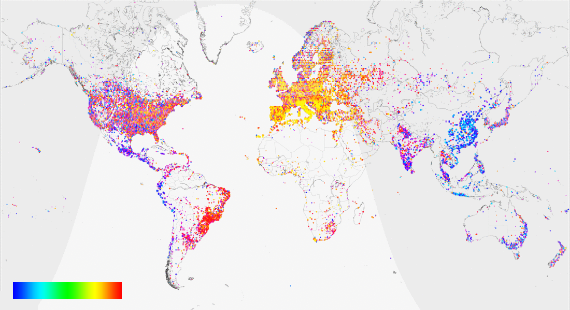
\includegraphics{figs/nettraffic-a.png}} &
            \resizebox{70mm}{!}{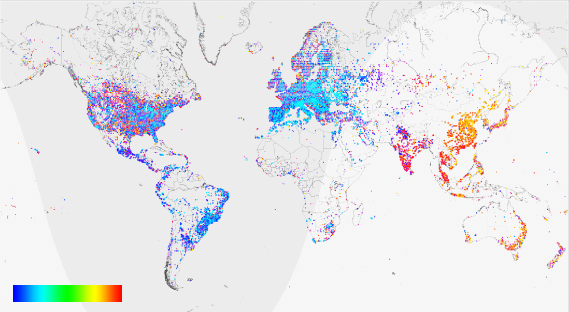
\includegraphics{figs/nettraffic-b.png}} \\
            \scriptsize{(a)\vspace{2mm}} &
            \scriptsize{(b)}    
        \end{tabular}
        \caption{Worldwide Internet traffic~\cite{internet:huffpost:nettraffic}. Daytime Internet usage in (a) western (b) eastern hemisphere}
        \label{fig:intro:nettraffic}
    \end{center}
\end{figure}

As another example, let us consider profiling of phone users based on the phone usages. Typically, young people are more inclined towards using data services rather than voice services while professionals and elderly people mostly use voice services. Thus, the profiling algorithm should consider these differences in rates in which different user groups are using the services.

To get a clearer picture of the locality of data activation and rate in which data are generated, let's consider the social media statistics. As of the second quarter of 2015, Facebook had 1.49 billion monthly active users. In the third quarter of 2012, the number of active Facebook users had surpassed 1 billion. Active users are those who logged into Facebook during the last 30 days. It was only on the August 28, 2015, that Facebook had 1 billion users on a single day. Let us assume that we want to do a sentiment analysis over the data collected from a week of activity in Facebook. Even though the class distribution (positive and negative sentiments)  may remain balanced, however, more active users will clearly ``overshadow'' the inputs given by the less active users. Similarly, about 300 million users produce 500 million tweets per day on Twitter. Figure~\ref{fig:intro:tweets} shows tweets for 5 different hashtags, namely, \#Trump, \#Syria, \#football, \#Volkswagen, and \#eclipse for the period of Aug 29, 2015 - Sept 28, 2015 (\cite{internet:topsy:tweets}). 
\begin{figure}[htbp] 
    \begin{center}
            \resizebox{110mm}{!}{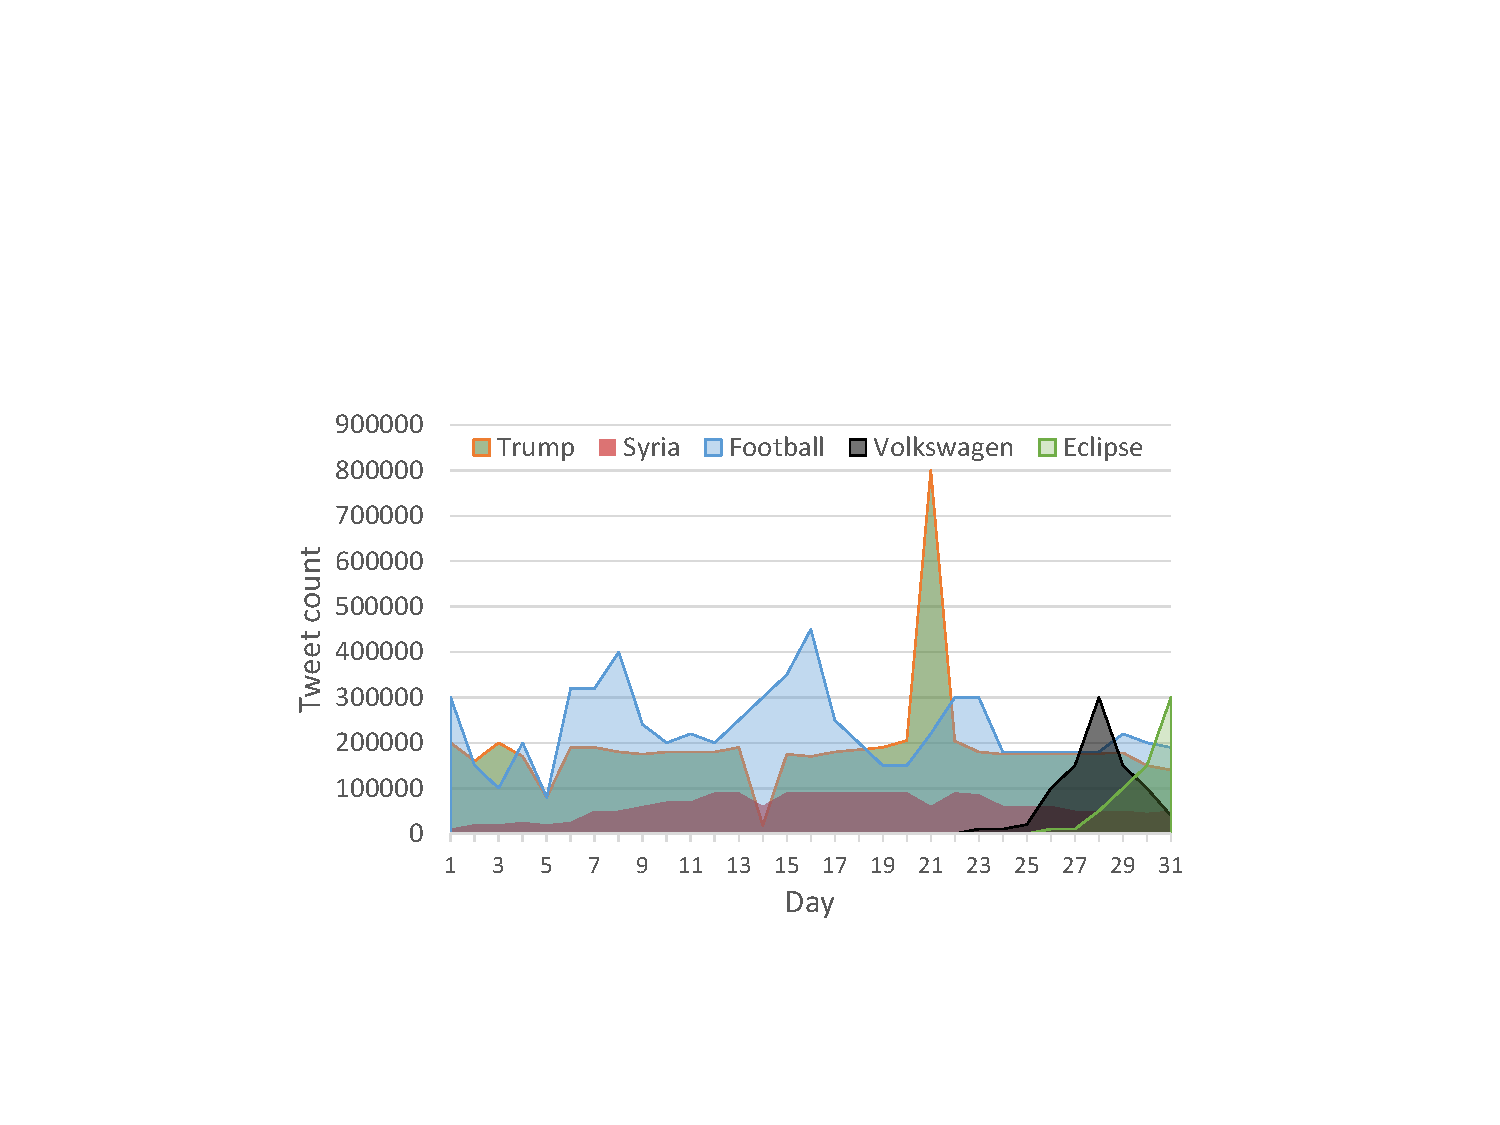
\includegraphics{figs/tweets.pdf}}
        \caption{Number of tweets for different hashtags }
        \label{fig:intro:tweets}
    \end{center}
\end{figure}
\noindent As it can be seen, \#football has a weekly repetitive trend, most certainly because of weekend games. \#Trump (USA's presidential candidate for 2016), on the other hand, has a steady rate with occasional spikes depending on some highlighted events, e.g., debate. The topic \#Syria has lower rate, however, it has a steady flow. Owing to the news of carbon emission from Volkswagen cars and lunar eclipse of September 28, 2015, topics like \#Volkswagen and \#eclipse got trending, however, they are expected to disappear soon. If each of these topics is to be treated equally, slower but consistent streams like \#Syria would suffer from lack of data volume. 

Based on the discussion above, it is evident that these streams do not necessarily follow a uniform distribution. Rather, these streams can be considered as a collection of many sub-streams, with following properties:
\begin{itemize}
    \item Slow sub-streams generating low but relatively consistent number of data, e.g., \#Syria.
    \item Alternating sub-streams generating moderate number of data. Activation of sub-streams within the set is dependent on each other, e.g., streams related to the football clubs.
    \item Sub-streams that produce a very large amount of data but remain active for only very short periods of time, e.g., \#eclipse.
\end{itemize}

Applying machine learning methods in such streams without considering the differences in the rate of data incoming from different sub-streams might lead to a set of decision rules dominated by the sub-streams with the highest number of instances. Moreover, most stream mining algorithms only keep track of most recent incoming instances and forget older data. Such algorithms would thus forget important decision rules learned over longer periods of time for slow but consistent sub-streams when a heavy burst of occasional sub-streams arrives. It would take a long time to learn the same rules again. Similarly, a burst could lead to the deletion of decision rules for recurring sub-streams too. This could significantly affect the performance of the models. Even for slow sub-streams the overall performance measures may not reflect poor decision performances for those slow sub-stream, as the number of instances belonging to those streams is not high. But, ideally we would expect that the mining algorithms should be effective for the entire data space.

In this thesis, we address such scenarios. To the best of our knowledge no previous work has specifically addressed this issue. In most works, the evaluation is performed with randomized streams, and concept drift, concept evolution, concept recurrence, etc. are addressed within the randomized stream. We extend one such data generation algorithm to implement the scenario presented above. Empirical evaluation is performed to compare the performances of existing algorithms for such streams. Comparing the results with the results from general randomized streams, it is found that existing algorithms do not perform at their best for streams with high temporal locality. Thus, this thesis presents an ensemble algorithm derived from one of the state-of-the-art algorithms to improve its performance in such scenarios. Extensive evaluation shows that the new method achieves more stable results and overcomes the challenges posed by the nature of the stream. It also retains all the positive factors of the original algorithm.

The next section discusses the basic idea of the algorithm without going into mathematical details. We present the algorithm later in great detail once the related literature and the concepts are introduced in the next couple of chapters.

\section{Intuition}
\label{sec:intro:intu}
The central idea of our method is based on the primal decision tree adaption by Domingos and Hulten~\cite{domingos00:vfdt} for streams named Very Fast Decision Tree (VFDT), also commonly known as Hoeffding Tree (HT). Their method is based on the assumption that to find the best attribute for a split decision at any node in a decision tree, it would be sufficient to consider only a certain amount of training data on that node. The Hoeffding bound~\cite{hoeffding63:bound} is a measurement for the degree of certainty for such an approach, which gives an error bound for a decision taken after seeing a certain amount of instances. This bound essentially states that any decision taken after observing a certain amount of instances would remain the same after seeing an infinite number of instances and the error margin can be computed with this bound. A detailed discussion of this bound and the algorithm is presented in Chapter~\ref{chp:background}.

With such an approach, challenges posed by high volumes of data can be avoided as we do not need to remember all the observed data instances. Rather, the statistics of the instances are sufficient to effectively decide about a split attribute. One of the limitations of a Hoeffding Tree is that it grows linearly as the time passes or as the instances arrive in the system. The root of the tree is the node that is used for splitting the oldest set of examples. Similarly, decision rules at lower levels also become old, while the leaves contain information from the most recent instances. To keep the rules updated numerous approaches such as resetting the tree, pruning bad performing nodes, etc., have been proposed. A detailed discussion of adaptations for concept drift, evolution, recurrence, etc. is presented in Chapter~\ref{chp:background}.

With the reset and pruning property, the Hoeffding Tree exhibits a special property, in particular. It always adapts itself for the newer examples. The number of examples upon which the HT's decision rules depend on is directly related to the size of the tree and the number of examples required to split a node. The number of decision or split nodes could be a measurement of the size of the tree. A smaller tree would adapt faster to the changes in the data, whereas, a larger tree would take longer time to adapt. Using this rationale a bagging method based on different sized trees is proposed by Bifet et al.~\cite{bifet09:asht}. In this method, a fixed number of Hoeffding Trees with different size (number of decision nodes) limits are used. Each time a tree exceeds the size threshold, the tree gets reset. Trivially, smaller trees would reset more often than the larger trees, and thus, the decision rules from smaller trees will base on the most recent data. Larger trees, however, would contain decision rules from older data.

We combined these concepts to address our problem. First, we introduced a size restricted variant of Hoeffding Tree named Size Restricted Hoeffding Tree (SRHT). Unlike its predecessor Adaptive Size Hoeffding Tree~\cite{bifet09:asht}, SRHT does not get reset immediately after it reaches the size limit. Instead, it stops growing i.e. no further split occurs, however, the weights in the leaf nodes are updated with incoming instances. It also combines two different concepts introduced by its predecessors: (i) it resets once a size limit is reached and (ii) it maintains alternate trees or subtrees when necessary. Thus, even after reaching the size limit, a tree can switch to its alternate tree and start growing again. This ensures that the model would remain updated to some extent in a drifting environment, even though the tree growth would be restricted.

We use this setup in a modified bagging scheme introduced in~\cite{bifet09:asht}. Similar to the Hoeffding Tree, a smaller SRHT will have decision rules for most recent data, and a larger tree would contain rules for some older instances, too. In our problem's context, a smaller tree would have decisions for high speed sub-streams or burst of incoming streams. Whereas only the larger trees will have some decision rules for slow but consistent sub-streams, along with the decision rules for most recent data. This is because, the recent data are always dominated by high speed sub-streams. Smaller data portions do not contain enough information about the slow streams or enough examples from slow streams to decide on them. Keeping this in mind, we control the reset of larger trees to keep hard-learned decision rules (hard in terms of time required). In doing so, we maintain an alternate pool of trees that are to be reset soon, and we start to maintain a new tree with same size limit from scratch. For the transition time we consider votes from all the trees, thus effectively increasing the weights for slower streams. In Chapter~\ref{chp:algo}, we present more elaborate description of the proposed approach.

\section{Related Works}
\label{chp:relworks}
Compared to data mining, stream mining is a young area. Most of the methods date back only a couple of decades. Similarly, the concept of ensemble learning was first introduced in the traditional batch learning, however, ensemble adaptations for streams are fairly new concepts. In this chapter, we list the most influential methods developed so far with particular focus on tree based learners. We follow a rudimentary narrating style starting directly with methods for general stream learners for stationary streams, and then for evolving data streams. After that, we list the base methods for ensemble learning, and finally we present ensemble based stream learners.

\subsection{Stream Mining}
%Compared to the classical data mining approaches stream mining is relatively a newer topic to be addressed in literature. Even though for batch approaches both classification and clustering problems have been vastly studied, their stream adaption remains a challenge due the restrictions imposed by the stream data. Possibility of temporal locality makes the classification problem harder in a streaming environment. Algorithms needs to address the evolution of underlying data stream. 

Domingos and Hulten introduced a strict one-pass adaptation of decision tree approach~\cite{breiman84:dt,quinlan93:c45} for data streams. Classic approaches like ID3 and C4.5 learners assume that all training examples can be stored in the main memory altogether. This is a significant limitation to the number of examples these algorithms can handle. Similarly, disk based decision tree learners (SLIQ~\cite{mehta96:sliq}, SPRINT~\cite{shafer96:sprint}, etc.) become very expensive when data sets are very large and the expected trees has many levels. Domingos and Hulten proposed \textit{Very Fast Decision Trees (VFDT)}~\cite{domingos00:vfdt} that uses the Hoeffding bound~\cite{hoeffding63:bound} to build an anytime decision tree for constant memory and time. The primary assumption in this approach is that to find the best attribute for a node in a decision tree, it may be sufficient to consider only a fraction of the training set that passes through that node. The Hoeffding bound provides a statistical measure to determine how much data is needed to ensure a level of degree of certainty, i.e. the error margin would be bounded by a given value~\cite{catlett91:thesis}.

Like most statistical and machine learning algorithms VFDT assumes that training data is randomly drawn from a stationary distribution. This assumption is not valid for large databases and data streams. Over time an underlying method or environment that generates data could change. The shift is  referred to as {\it concept drift} in the literature and can be abrupt as well as very slow. Data related to weather forecast, economic condition prediction, mis-calibrated sensors, etc. are examples of a concept drifting environment. A concept-adaptive variant of VFDT, \textit{CVFDT}~\cite{hulten01:cvfdt}, can handle such scenarios. CVFDT updates its decision rules, essentially the tree structure, by detecting the concept drift in the data. It maintains alternate subtrees whenever an old subtree becomes questionable, and replaces the old one with the alternative when it becomes more accurate. CVFDT uses a sliding window and updates sufficient statistics by increasing the count of newly arrived examples and decreasing the count of old examples in the window. Essentially CVFDT achieves same accuracy that would be achieved if VFDT had been run again with the new data. CVFDT does this in $O(1)$ time with an additional space requirement as compared to the VFDT's $O(w)$ complexity where $w$ is the window size. Another extension of VFDT, VFDTc was proposed in~\cite{gama05:vfdtc} that improves VFDT by handling continuous numeric attributes and adding na\"ive Bayes prediction at the leaves of the tree.


% TODO: briefly include multi-label evolving ...
% TODO: frequent item set mining]

\subsection{Ensemble Learning}
Traditional machine learning algorithms generally feature a single model or classifier such as \textit{na\"ive Bayes} or \textit{multilayer perceptron (MLP)}. The free parameters of these learners (e.g. weights of feed-forward neural network) are set by realizing the complete training set. These classifiers provide a measurement of the generalization performance i.e. how well the classifier generalizes the training set. However, given a finite set of training example, it is rather reasonable to assume that the data might contain several generalizations. For example, a different setting of the neural network classifier (weights, node layers, node counts, etc.) changes the final network to some extent. For stream environment, this assumption becomes trivial. Thus, choosing a single classifier is not always optimal. Using the best classifier among several classifiers where each is trained with the same training set would be an alternative, however, information is still being lost by discarding sub-optimal options. A better alternative would be to build a classifier ensemble. Ensemble classifiers combine the prediction of multiple base level models built on traditional algorithms. A simple process for combining the predictions could be to choose the decision based on majority voting~\cite{parhami94:voting}. As demonstrated in several works~\cite{breiman93:regression, schapire90:whyens, wolpert92:whyens}, ensemble methods (e.g. ensembles of neural networks)~\cite{hansen90:ensNN, tumer99:whyens} yield better performance. 

Without proper selection and control over the training process of the base learners, ensemble classifiers could result in poorer performance. Simply choosing a base classifier and training it for several settings would surely produce highly correlated classifiers which would have adverse effect on the overall ensemble process. One solution of this  is to train each classifier with its own training set generated by random sampling of the original one. However, with random sampling each classifier would receive a reduced number of training patterns, resulting in a reduction of the accuracy of the individual base classifier. This reduction in the base classifier accuracy is generally not recovered by the gain of combining the classifiers unless measures are taken to make the base classifiers \textit{diverse}. Classifiers with complementary information would give the lowest correlation~\cite{breiman93:regression, tumer99:whyens}. Many methods have been proposed to promote diversity among the base classifier: \textit{bagging}~\cite{breiman94:bagging}, \textit{boosting}~\cite{drucker94:boosting, freund97:boosting, oza99:whyens}, \textit{cross-validation partitioning}~\cite{krogh95:ensNNcv, tumer99:whyens}, etc. These methods mainly process the entire training set repeatedly and require at least one pass for each base model. This is not suitable for streaming scenarios. Stream adaptation of bagging and boosting methods has been introduced by Oza et al.~\cite{oza01:obagboost,oza01:thesis}.

\subsection{Ensemble Learning in Streams}
Learning algorithms in data streams require maintenance of a set of hypotheses based on the training instances seen thus far with the need for storage and reprocessing. Facilitating this requirement, Oza and Russell developed an online version~\cite{oza01:obagboost, oza01:thesis} of traditional bagging and boosting. Bagging works by randomly sampling with replacement from the training set to form a given number of intermediate training sets which are used to train same number of classifiers. During testing a majority voting scheme is employed on the decisions of all classifiers to deduce the final decision. Boosting uses an iterative procedure to adaptively change the distribution of training data by focusing more precisely on misclassified instances. Initially all instances have equal weights, and at the end of a boosting round the weight of each instance is updated by increasing or decreasing if the instance was classified wrongly or correctly, respectively. For the \textit{online} variant of these algorithms, not knowing the size of the training data poses a problem in determining the size of training sets to build the base models. In~\cite{oza01:obagboost} the authors address this situation by training $k$ models with each instances where $k$ is a suitable Poisson random variable. Later on,~\cite{pelossof08:boosting} proposed the \textit{Online Coordinate Boosting} algorithm where the number of weight updates of~\cite{oza01:obagboost} is reduced using few simple alterations.


As mentioned in the previous section, a \textit{Hoeffding Tree (HT)} i.e. VFDT~\cite{domingos00:vfdt}, can be used to build classifiers for concept drifting streams. The Hoeffding Tree has the property that it adapts itself for the newer examples. The number of examples that a HT is built upon is determined by two numbers: (i) the  size of the tree, and (ii) the number of examples used to create a node. Thus, smaller trees adapt faster to the changes in the data, while larger trees try to retain the rules that reflect longer time-frame, simply because they are built on more data. In other words a tree bounded by size $n$ would be reset twice as often as tree bounded by size $2n$. \textit{Adaptive Size Hoeffding Tree (ASHT)} bagging~\cite{bifet09:asht}, uses this intuition to build an ensemble of classifiers of different sized Hoeffding trees. ASHT bagging attempts to increase the diversity in the bagging approach. The maximum allowed size for the $n$-th tree is twice the size of the $(n-1)$-th, where the first tree has a size of $2$. Additionally, the inverse of the squared errors have been used as the weights for the trees. Authors made an observation that bagging using 5 trees of different size might be sufficient to gain higher accuracy, as the error level for bagging with more trees does not improve much but takes longer time.

Same authors also proposed an adaptive window size bagging method-- \textit{ADWIN}~\cite{bifet09:asht}. ADWIN automatically detects and adapts to the current rate of change. To do so ADWIN adapts its window size to maximize the statistically consistently length that conforms following hypothesis ``there has been no change in the average value inside the window''. The window is not maintained explicitly, rather using a variant of an exponential histogram technique that takes $O(log\;w)$ memory and $O(log\;w)$ processing time where $w$ is the length of the window. Experimental evaluation showed that ADWIN bagging has better accuracy than ASHT bagging, however, requires more time and memory. 

ADWIN has later been used in \textit{leverage bagging}~\cite{bifet10:levbag}. Leverage bagging improves randomization by increasing the re-sampling and using output detection codes. Re-sampling with replacement is done in online Bagging using Poisson(1)~\cite{oza01:obagboost}. Instead leverage bagging increases the weights of re-sampling using a larger value $\lambda$ to compute the value of the Poisson distribution. The Poisson distribution is used to model the number of events occurring within a given time interval. Randomization is added at the output of the ensemble using output codes. This method works by assigning a binary string of length $n$ to each class and building an ensemble of $n$ binary classifiers. Each of the classifiers learns one bit for each position in the string. A new instance is classified to the class with the closest binary code. 

ADWIN has also been used in building ensembles of \textit{Restricted Hoeffding Trees}~\cite{bifet10:rht}. A mechanism for setting the learning rate of perceptrons in the base neural network learner using the ADWIN change detection method is used to restrict the tree. Additionally, a mechanism for resetting a member tree is also been introduced when a particular member is no longer performing well. The method outperforms traditional bagging in terms of accuracy, but requires additional memory and time.



\section{Thesis Objectives}
The primary objective of this thesis is to devise an algorithm realizing the intuitions discussed earlier. In doing so, an extensive survey of existing literature is performed. The most relevant portion of which has already been discussed in the previous section. The remaining is attached at the end of the thesis (see Appendix~\ref{appndx:erw}). This thesis presents a new way to look at the composition of various real-world streams e.g. social networks. Based on that, a new approach of data generation to facilitate slow, fast, burst, recurrent, etc. behavior in a randomized data stream is proposed. In an effort to combine the ideas of Adaptive Size Hoeffding Tree and Adaptive Hoeffding Tree using ADWIN, a new ensemble method is devised aiming to improve the performance of slower streams. Lastly, a comprehensive empirical comparison of current Hoeffding tree-based approaches is performed.


\section{Outline}
The rest of the article is organized as follows: Chapter~\ref{chp:background} presents the base concepts required for the thesis. We first discuss the basic streaming adaptations of batch methods, and later their usages in ensemble approaches. Chapter~\ref{chp:algo} precisely defines the problem and discusses the development of our algorithm addressing the motivation and intuition of this chapter. In Chapter~\ref{chp:dataset} existing data set generators are discussed first and a new data generation scheme is explained that fulfills the requirements discussed in the intuition section (Section~\ref{sec:intro:intu}). Finally, before concluding the thesis in Chapter~\ref{chp:conclude}, in Chapter~\ref{chp:exp} we describe the experimental evaluation process and findings. Extensive evaluation is performed to compare existing methods, as well as, the newly developed method. 

%\section{Related Works}
\label{chp:relworks}
Compared to data mining, stream mining is a young area. Most of the methods date back only a couple of decades. Similarly, the concept of ensemble learning was first introduced in the traditional batch learning, however, ensemble adaptations for streams are fairly new concepts. In this chapter, we list the most influential methods developed so far with particular focus on tree based learners. We follow a rudimentary narrating style starting directly with methods for general stream learners for stationary streams, and then for evolving data streams. After that, we list the base methods for ensemble learning, and finally we present ensemble based stream learners.

\subsection{Stream Mining}
%Compared to the classical data mining approaches stream mining is relatively a newer topic to be addressed in literature. Even though for batch approaches both classification and clustering problems have been vastly studied, their stream adaption remains a challenge due the restrictions imposed by the stream data. Possibility of temporal locality makes the classification problem harder in a streaming environment. Algorithms needs to address the evolution of underlying data stream. 

Domingos and Hulten introduced a strict one-pass adaptation of decision tree approach~\cite{breiman84:dt,quinlan93:c45} for data streams. Classic approaches like ID3 and C4.5 learners assume that all training examples can be stored in the main memory altogether. This is a significant limitation to the number of examples these algorithms can handle. Similarly, disk based decision tree learners (SLIQ~\cite{mehta96:sliq}, SPRINT~\cite{shafer96:sprint}, etc.) become very expensive when data sets are very large and the expected trees has many levels. Domingos and Hulten proposed \textit{Very Fast Decision Trees (VFDT)}~\cite{domingos00:vfdt} that uses the Hoeffding bound~\cite{hoeffding63:bound} to build an anytime decision tree for constant memory and time. The primary assumption in this approach is that to find the best attribute for a node in a decision tree, it may be sufficient to consider only a fraction of the training set that passes through that node. The Hoeffding bound provides a statistical measure to determine how much data is needed to ensure a level of degree of certainty, i.e. the error margin would be bounded by a given value~\cite{catlett91:thesis}.

Like most statistical and machine learning algorithms VFDT assumes that training data is randomly drawn from a stationary distribution. This assumption is not valid for large databases and data streams. Over time an underlying method or environment that generates data could change. The shift is  referred to as {\it concept drift} in the literature and can be abrupt as well as very slow. Data related to weather forecast, economic condition prediction, mis-calibrated sensors, etc. are examples of a concept drifting environment. A concept-adaptive variant of VFDT, \textit{CVFDT}~\cite{hulten01:cvfdt}, can handle such scenarios. CVFDT updates its decision rules, essentially the tree structure, by detecting the concept drift in the data. It maintains alternate subtrees whenever an old subtree becomes questionable, and replaces the old one with the alternative when it becomes more accurate. CVFDT uses a sliding window and updates sufficient statistics by increasing the count of newly arrived examples and decreasing the count of old examples in the window. Essentially CVFDT achieves same accuracy that would be achieved if VFDT had been run again with the new data. CVFDT does this in $O(1)$ time with an additional space requirement as compared to the VFDT's $O(w)$ complexity where $w$ is the window size. Another extension of VFDT, VFDTc was proposed in~\cite{gama05:vfdtc} that improves VFDT by handling continuous numeric attributes and adding na\"ive Bayes prediction at the leaves of the tree.


% TODO: briefly include multi-label evolving ...
% TODO: frequent item set mining]

\subsection{Ensemble Learning}
Traditional machine learning algorithms generally feature a single model or classifier such as \textit{na\"ive Bayes} or \textit{multilayer perceptron (MLP)}. The free parameters of these learners (e.g. weights of feed-forward neural network) are set by realizing the complete training set. These classifiers provide a measurement of the generalization performance i.e. how well the classifier generalizes the training set. However, given a finite set of training example, it is rather reasonable to assume that the data might contain several generalizations. For example, a different setting of the neural network classifier (weights, node layers, node counts, etc.) changes the final network to some extent. For stream environment, this assumption becomes trivial. Thus, choosing a single classifier is not always optimal. Using the best classifier among several classifiers where each is trained with the same training set would be an alternative, however, information is still being lost by discarding sub-optimal options. A better alternative would be to build a classifier ensemble. Ensemble classifiers combine the prediction of multiple base level models built on traditional algorithms. A simple process for combining the predictions could be to choose the decision based on majority voting~\cite{parhami94:voting}. As demonstrated in several works~\cite{breiman93:regression, schapire90:whyens, wolpert92:whyens}, ensemble methods (e.g. ensembles of neural networks)~\cite{hansen90:ensNN, tumer99:whyens} yield better performance. 

Without proper selection and control over the training process of the base learners, ensemble classifiers could result in poorer performance. Simply choosing a base classifier and training it for several settings would surely produce highly correlated classifiers which would have adverse effect on the overall ensemble process. One solution of this  is to train each classifier with its own training set generated by random sampling of the original one. However, with random sampling each classifier would receive a reduced number of training patterns, resulting in a reduction of the accuracy of the individual base classifier. This reduction in the base classifier accuracy is generally not recovered by the gain of combining the classifiers unless measures are taken to make the base classifiers \textit{diverse}. Classifiers with complementary information would give the lowest correlation~\cite{breiman93:regression, tumer99:whyens}. Many methods have been proposed to promote diversity among the base classifier: \textit{bagging}~\cite{breiman94:bagging}, \textit{boosting}~\cite{drucker94:boosting, freund97:boosting, oza99:whyens}, \textit{cross-validation partitioning}~\cite{krogh95:ensNNcv, tumer99:whyens}, etc. These methods mainly process the entire training set repeatedly and require at least one pass for each base model. This is not suitable for streaming scenarios. Stream adaptation of bagging and boosting methods has been introduced by Oza et al.~\cite{oza01:obagboost,oza01:thesis}.

\subsection{Ensemble Learning in Streams}
Learning algorithms in data streams require maintenance of a set of hypotheses based on the training instances seen thus far with the need for storage and reprocessing. Facilitating this requirement, Oza and Russell developed an online version~\cite{oza01:obagboost, oza01:thesis} of traditional bagging and boosting. Bagging works by randomly sampling with replacement from the training set to form a given number of intermediate training sets which are used to train same number of classifiers. During testing a majority voting scheme is employed on the decisions of all classifiers to deduce the final decision. Boosting uses an iterative procedure to adaptively change the distribution of training data by focusing more precisely on misclassified instances. Initially all instances have equal weights, and at the end of a boosting round the weight of each instance is updated by increasing or decreasing if the instance was classified wrongly or correctly, respectively. For the \textit{online} variant of these algorithms, not knowing the size of the training data poses a problem in determining the size of training sets to build the base models. In~\cite{oza01:obagboost} the authors address this situation by training $k$ models with each instances where $k$ is a suitable Poisson random variable. Later on,~\cite{pelossof08:boosting} proposed the \textit{Online Coordinate Boosting} algorithm where the number of weight updates of~\cite{oza01:obagboost} is reduced using few simple alterations.


As mentioned in the previous section, a \textit{Hoeffding Tree (HT)} i.e. VFDT~\cite{domingos00:vfdt}, can be used to build classifiers for concept drifting streams. The Hoeffding Tree has the property that it adapts itself for the newer examples. The number of examples that a HT is built upon is determined by two numbers: (i) the  size of the tree, and (ii) the number of examples used to create a node. Thus, smaller trees adapt faster to the changes in the data, while larger trees try to retain the rules that reflect longer time-frame, simply because they are built on more data. In other words a tree bounded by size $n$ would be reset twice as often as tree bounded by size $2n$. \textit{Adaptive Size Hoeffding Tree (ASHT)} bagging~\cite{bifet09:asht}, uses this intuition to build an ensemble of classifiers of different sized Hoeffding trees. ASHT bagging attempts to increase the diversity in the bagging approach. The maximum allowed size for the $n$-th tree is twice the size of the $(n-1)$-th, where the first tree has a size of $2$. Additionally, the inverse of the squared errors have been used as the weights for the trees. Authors made an observation that bagging using 5 trees of different size might be sufficient to gain higher accuracy, as the error level for bagging with more trees does not improve much but takes longer time.

Same authors also proposed an adaptive window size bagging method-- \textit{ADWIN}~\cite{bifet09:asht}. ADWIN automatically detects and adapts to the current rate of change. To do so ADWIN adapts its window size to maximize the statistically consistently length that conforms following hypothesis ``there has been no change in the average value inside the window''. The window is not maintained explicitly, rather using a variant of an exponential histogram technique that takes $O(log\;w)$ memory and $O(log\;w)$ processing time where $w$ is the length of the window. Experimental evaluation showed that ADWIN bagging has better accuracy than ASHT bagging, however, requires more time and memory. 

ADWIN has later been used in \textit{leverage bagging}~\cite{bifet10:levbag}. Leverage bagging improves randomization by increasing the re-sampling and using output detection codes. Re-sampling with replacement is done in online Bagging using Poisson(1)~\cite{oza01:obagboost}. Instead leverage bagging increases the weights of re-sampling using a larger value $\lambda$ to compute the value of the Poisson distribution. The Poisson distribution is used to model the number of events occurring within a given time interval. Randomization is added at the output of the ensemble using output codes. This method works by assigning a binary string of length $n$ to each class and building an ensemble of $n$ binary classifiers. Each of the classifiers learns one bit for each position in the string. A new instance is classified to the class with the closest binary code. 

ADWIN has also been used in building ensembles of \textit{Restricted Hoeffding Trees}~\cite{bifet10:rht}. A mechanism for setting the learning rate of perceptrons in the base neural network learner using the ADWIN change detection method is used to restrict the tree. Additionally, a mechanism for resetting a member tree is also been introduced when a particular member is no longer performing well. The method outperforms traditional bagging in terms of accuracy, but requires additional memory and time.


\chapter{Background}
\label{chp:background}
This chapter discusses the primitives of data and stream classification. First, a brief overview of traditional data classification methods are presented. Followed by a section on data stream classification where challenges and approaches for stream classification are introduced. Finally, overview of current state-of-the-art ensemble learning methods are discussed. These discussion are lays the foundation of the approach introduced in this thesis.

\section{Learning Algorithms}
\label{sec:bg:learningalgos}
The goal of data classification process is to predict an outcome based on some give data. In order to do so, data mining algorithms first processes a training set containing a set of attributes and corresponding outcome: a class or a value. Algorithms develop hypotheses that best describe the relationship among the attributes and the outcome for the total instance set.  Formally, learning problems are defined as follow: Given a data set of $m$ instances  $D \equiv \{ \{\vec{x}_1, y_1\}, \{\vec{x}_2, y_2\}, \{\vec{x}_3, y_3\}, \dots, \{\vec{x}_m, y_m\} \}$ where $ \vec{x} = \{x_1, x_2, x_3, \dots, x_n\}$, learning algorithms try to approximate $H \equiv y = f(\vec{x})$. Additional to being typical linear, polynomial, etc. functions, $H$ can also be a set of IF-THEN rules. These rules or functions are then used to predict unseen instances where outcome class is not known. These algorithms are known as learning algorithms, and in last few decades, have widely been researched in the field of machine learning. This section briefly discusses few of the basic algorithms upon which the foundation of ensemble methods and this thesis are laid. The detailed discussion of these algorithms are out of the scope of this chapter. Thus we discuss only the core concepts here.

\subsection{$k$-Nearest Neighbors}
$k$-nearest neighbor algorithm, in short $k$-NN, is one the simplest learning available. It is a non-parametric instance-based lazy learning algorithm and works for both supervised and unsupervised learning. It uses similarity measure like distance functions to classify unknown instances. The decision is a majority voting of  $k$ neighbors where $k$ is predefined. For example, if $k= 1$ then an unknown instance is assigned the class label of its nearest neighbor. There are several schemes to find the $k$ nearest neighbors. For continuous data, some well-known distance functions are Euclidean distance, Manhattan distance, Minkowski distance, etc.
\begin{itemize}
    \item Euclidean distance $D_E = \sqrt{\sum_{\i =1 }^{k} (x_i - y_i)^2}$
    \item Manhattan distance $D_M = \sum_{\i =1 }^{k} |(x_i - y_i)|$
    \item Minkowski distance $D_{Mink}\sqrt[q]{\sum_{\i =1 }^{k} (|x_i - y_i|)^q}$
\end{itemize}
For categorical data, Hamming distance can be used. Hamming distance is defined as $D_H = \sum_{\i =1 }^{k} |(x_i - y_i)|$ where $|x_i - y_i|$ is $0$ if $x=y$, $1$ otherwise.

\begin{figure}[htbp]
    \begin{center}
        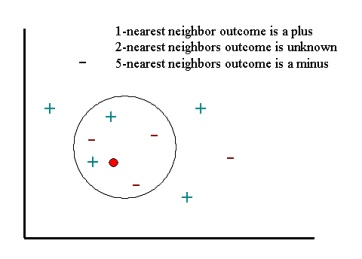
\includegraphics[width=3.0in]{figs/knn.jpg}
        \caption{Concept of $k$-NN}
        \label{fig:bg:knn}
    \end{center}
\end{figure}

Choosing an optimal $k$ is the prime challenge of $k$-NN algorithm, which is extremely training data dependent. Changing position of few training points could lead to a significant loss in performance. The method is particularly not stable in the class boundary. $k$ should be large enough that $k$-NN could overcome the noises in data, and small enough that instances of other classes are not included. Generally, higher $k$ reduces the overall noise and should be more precise. For most data set a value between $3$-$10$ performs much better than $1$-NN. Typically cross-validation is used to determine a good $k$. 

\subsection{Na\"ive Bayes}
Naive Bayes classification is based on Bayes rule. Bayes rule says that the probability of event $x$ conditioned on knowing event $y$, i.e. the probability of $x$ given $y$ is defined as
\[
    p(x|y) = \frac{p(x,y)}{p(y)} = \frac{p(y|x) p(x)}{p(y)}
\]
The naive Bayes classifier~\cite{langley92:nb} assumes that all the explanatory variables are independent. Given a feature set $X = x_1, x_2, \dots, x_n$ of $n$ independent variables, naive Bayes assigns the instances to $k$ possible outcome or classes, $p(C_k | X)$. Using Bayes rule, the conditional probability can be decomposed as:
\[
    p(C_k |X) = \frac{p(C_k) p(X|C_k)}{p(X)}.
\]
In other words,
\[
    posterior = \frac{prior \times likelihood}{evidence}.
\]
Using chain rule repetitively, it can be expressed as follows:
\[
    p(C_k |X) = p(C_k) \prod_{i=1}^n p(x_i | C_k)
\]
The predicted class is the one which maximizes the conditional probabilities $p(C_k|X)$, that is, classifier assigns the class label $\hat{y} = C_k$ for some $k$ that satisfies:
\[
    \hat{y} = \underset{k \in \{1, \dots, K\}}{argmax}  p(C_k) \prod_{i=1}^n p(x_i | C_k)
\]

\subsection{Decision Tree}
Decision trees (DTs) are another popular genre of non-parametric supervised learning algorithms. Trees allow a way to graphically organize a sequential decision process. Decision tree, a directed acyclic graph, contains decision nodes, each with branches for all alternate decisions. Leaf nodes are labeled with respective class label. Each path from root to leaf is a decision rule, consisting of conditional part (unions of all internal nodes' conditions) and a decision (of leaf node).

Decision trees use {\it information gain} to select the splitting attribute that would maximize the total entropy of each of the subtrees resulting from the spit. Entropy is a measurement of purity of an attribute, typically ranged between 0 and 1. A pure attribute, attribute with definitive value-class relationship, would have a low entropy and is easy to predict. On the other hand attribute with highly mixed value-class relationship would yield high entropy. A common entropy function is-
\[
    entropy = - \sum_{i=1}^n p_i \lg p_i.
\]
where $p_1, p_2, \dots, p_n$ are the distributions of several class attributes and $\sum p_i = 1$. Information gain is the difference between old and new entropy after a split. This is good measurement of relevance of an attribute. However, in cases where an attribute can take on a large number of distinct values, information gain is not ideal. Presence of large set of values could uniquely identify the classes but also reduces chance to generalize unseen instance and should be avoided to be place near root.

Decision tree is, however, computationally feasible. Average cost of constructing a decision tree for $n$ instances with $m$ attributes is $O(mn \lg n)$, and querying time is $O(\lg n)$.

\subsection{Neural Network}
The Neural Network (NN) is a learning method inspired by biological neural network. A set of inter-connected nodes (also known as perceptrons and neurons) mimics biological neural network. Figure~\ref{fig:bg:nnlayer} shows a skeleton of a neural network. Neural network is a weighted directed graph where a input layer is connected to the output layer via some layers of hidden layers. This is commonly known as Multi-Layer Perceptron (MLP). Decisions are made looking only into the output layer only. Hidden layers enlarge the space of hypotheses. If there is no hidden layer, then neural network becomes a simple regression problem i.e. output is a linear function of inputs. Each connection among these nodes has an associated weight. Given an input data set, these weights are updated accordingly to best fit the classification model. Learning is done by back-propagation algorithm~\cite{raul96:nn}. Errors are propagated back from the output layer to the hidden layer and weights are updated to minimize error.
\begin{figure}[htbp]
    \begin{center}
        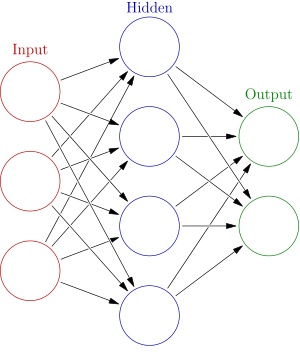
\includegraphics[width=4.0cm]{figs/nnlayers.png}
        \caption{Neural network layers}
        \label{fig:bg:nnlayer}
    \end{center}
\end{figure}

Learning starts with assigning a small value as initial weights to all the connection weights. In case of a single perceptron, learning process is analogous to moving a parametric hyperplane around. Let $w_i$ be the weight of $i$-th input, then after $t+1$ iteration weight $w_i(t+1) = w_i(t) + \nabla E_i(t)$, where $\nabla E_i$ is the gradient of the error function. For a input vector $\mathbf{x}$ and true output $y$, $E$ is defined as the squared error:
\[
    E = \frac{1}{2} Err^2 = \frac{1}{2} (y - h_w(\mathbf{x}))^2
\]
Thus gradient of $E$ would be:
\begin{align*}
    \nabla E = \frac{\partial E}{\partial W_j} & = Err \times \frac{\partial Err}{\partial W_j} = Err \times \frac{\partial}{\partial W_j} (y - g(\sum_{j=0}^n w_j x_j)) \\
    & = - Err \times g^{\prime} (in) \times x_j
\end{align*}
Based on this, weight update rule would be:
\[
    w_j = w_j + \alpha \times Err \times g^{\prime} (in) \times x_j
\]
where $\alpha$ is learning rate coefficient. Back propagation algorithm for multi-layer perceptron also works in similar fashion. Weights in the output layer are updated using following equation:
\[
    w_{j,i} = w_{j,i} + \alpha \times a_j \times \nabla_i
\]
where $\nabla_i = Err \times g^\prime(in_i)$. Hidden layers propagates this error from the output layer using:
\begin{align*}
    \nabla_j &= g^\prime (in_i) \sum_i w_{j,i} \nabla_i \\
    w_{k, j} &= w_{k, j} + \alpha \times a_k \times \nabla_j
\end{align*}

MLP is a very expressive method. Only $1$ hidden layer is sufficient to represent all continuous functions and $2$ can represent any functions. MLP is prone to local minima, which is avoided by running MLP multiple times with different initial weight settings.

\section{Data Stream Classification}
Traditional data mining algorithms work in a memory bounded environment and require multiple scan of the training data. In stream environment, one of the major assumptions is that new data samples are introduced in the system with such a high rate that repetitive analysis becomes infeasible. Thus, for stream classification, algorithms should be able to look into a instance only once and decide upon that. A bounded memory buffer can be used to facilitate some level of repetition. However, which instances are to remember and which are to forget would then become a decision choice. An alternate choice is to maintain sufficient statistics to have a representation of the data. The process of deletion or summarization of instances, however, means that some information are being lost over the time.

In this section, these challenges are first discussed in details. Then it presents the basis of some of the concepts arisen to handle these challenges. Finally, before moving onto the ensemble leaning, it discusses current state-of-the-art algorithms for stream mining.

\subsection{Challenges}
Challenges posed by the streaming environment can be categorized into two groups: (i) relating to runtime and memory requirements and (ii) relating to underlying concept identification. Speed of incoming data, unbounded memory requirement, single-pass learning fall into the first category. On the other hand, lack of labeled data, concept drift, evolution and recurrence are examples of latter category.

\paragraph{Speed of data arrival:}
As mentioned before, it is an inherent characteristic of data streams that it arrives with a high speed. The algorithm should be able to adapt to the high speed nature of streaming information. The rate of building the classifier model should be higher than the data rate. This gives a very limited amount of available time for classification as compared to the traditional batch classification models.

\paragraph{Memory requirements:}
To apply traditional batched approaches in streaming data, an unbounded memory would be needed. This challenge has been addressed using load shedding, sampling, aggregation, etc. Rather than storing all the instances, algorithms store a subset of the data set or some statistical values or a combination of both which represents the data seen thus far. New instances can be classified only by looking into these stored information. 

\paragraph{Single-pass learning:}
The premise of this requirement is two-fold. First, as mentioned above, data would not be available in the memory after a short period of time due to the volume of data. Secondly, even if the data remain available, running a batched-like approach for millions of data points would highly increase the running time of the algorithm. To attain faster processing time with limited storage, algorithm should access the data stream only once, or a small number of times. Mining models must posses the capability to learn the underlying nature of data in a single pass over the data.

\paragraph{Lack of labeled data:}
Unlike most data sets or settings of batched approaches, steam mining data sets are often poorly labeled. A large number of experimentations are done with generated data set where the data generation process can easily be controlled to have proper labeling. However, in data set collected from real world are often lack this. For example, to setup a supervised learning experimentation using a data set collected from social media, e.g. Twitter, data needs to be first categorized by human intervention. Manual labeling of such data is often costly, both in terms of resources and time. In practice, only a small fraction of data is labeled by human experts or automated scripts. A stream classification algorithm is thus required to be able to predict after observing a small number of instances, i.e. to be ready to predict anytime.

\begin{figure}[htbp] 
    \begin{center}
        \begin{tabular}{cc}
            \resizebox{60mm}{!}{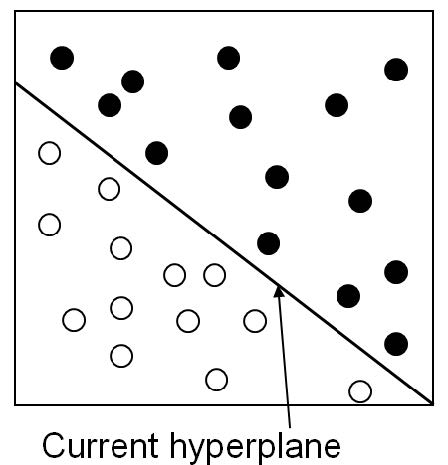
\includegraphics{figs/condrift-a.jpg}} &
            \resizebox{60mm}{!}{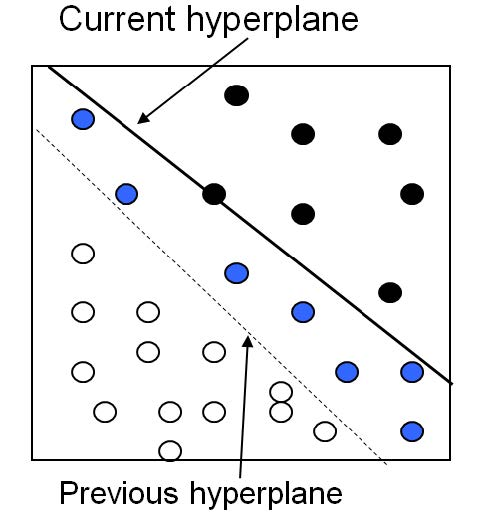
\includegraphics{figs/condrift-b.jpg}} \\
            \scriptsize{(a)\hspace{0mm}} & \scriptsize{(b)}    
        \end{tabular}
    \caption{Concept drift in data streams.}
    \label{fig:bg:condrift}
    \end{center}
\end{figure}
\paragraph{Concept drift:}
Concept drift is a statistical property of data streams where the target variable drifts away from the model that is trying to predict it. In other words the underlying data distribution is changing over time. As a result accuracy of the classifier model decreases over time. For example, buying pattern of the customers in a store changes over time, mostly due to the seasonality. Electrical and mechanical devices wear off over time, producing shifted result which would cause drift in the observing data. Learning models should adapt to these changes quickly and accurately. Let us consider the example in Figure~\ref{fig:bg:condrift}. As a new chunk arrives (Figure~\ref{fig:bg:condrift}a), a new classifier is learned. The decision boundary is denoted by the straight line. The positive examples are represented by unfilled circles while the negative examples are represented by filled circles. With time the concept of some of the examples may change. As shown in Figure~\ref{fig:bg:condrift}b, due to concept drift some negative examples may have become positive. So, the previous decision boundary has become outdated and a new model has to be learned. Formally, concept drift is the change in the joint probability \(P(X, y) = P(y|X) \times P(X)\). Thus, observing the change in $y$ for given $X$, i.e. $P(y|X)$ is the key for detection.

One challenge posed here is to differentiate the noise in data and the actual shift of the concept. Often in streaming environment data contains the both. Rate of drift is also a factor in detection. Sudden drift, known as {\it concept shift}, is easier to detect than concept drift, which is considered to be gradual.

\begin{figure}[htbp]
    \begin{center}
        \begin{tabular}{cc}
            \resizebox{60mm}{!}{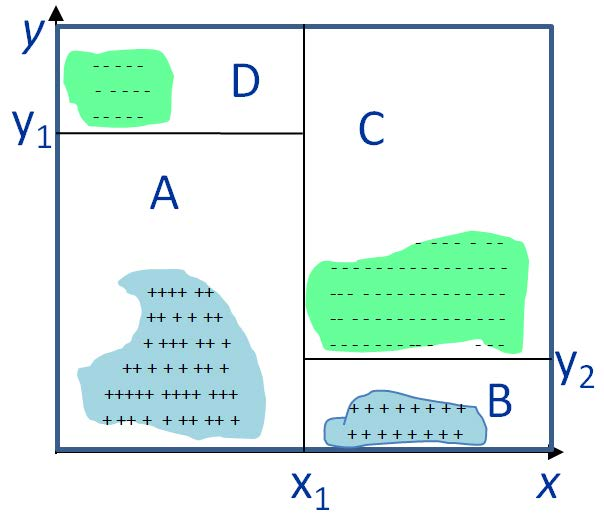
\includegraphics{figs/conevol-a.jpg}} &
            \resizebox{60mm}{!}{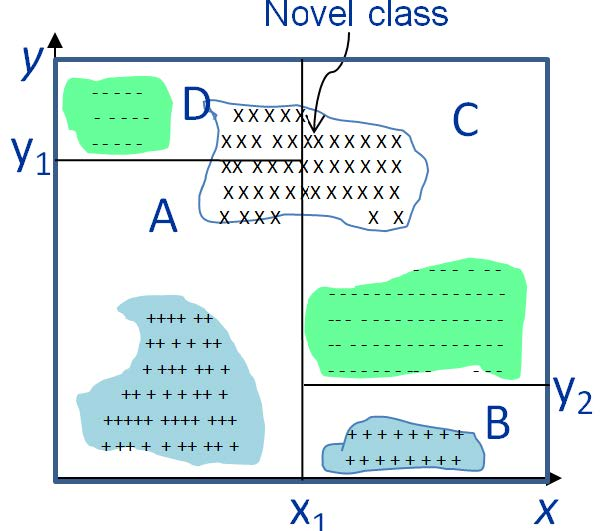
\includegraphics{figs/conevol-b.jpg}} \\
            \scriptsize{(a)\hspace{0mm}} & \scriptsize{(b)}    
        \end{tabular}
        \caption{Concept evolution in data streams.}
        \label{fig:bg:dataevol}
    \end{center}
\end{figure}
\paragraph{Concept evolution:}
Concept evolution is referred to the emergence of a new class or a set of classes in stream data as the time flows. Twitter stream is an ideal example where concept evolution is very easily identifiable. Twitter reacts, seemingly, very fast upon important news around the globe. Looking into the different hash tag usages in such social media currently trending topics can be identified. To present a clearer picture let's consider following example in Figure~\ref{fig:bg:dataevol}. At certain point of time four classes and their corresponding decision boundaries are shown in the Figure~ (\ref{fig:bg:dataevol}a). With the more incoming data a novel class emerges, and for that decision boundaries need updating. Emergence of new class can affect any number of decision boundary/ rule, from one to all.

Concept evolution is also prone to noise. Furthermore, clear distinction between drift and evolution might not always be possible, partially due the lack of unlabeled data.

\paragraph{Class recurrence:}
Class recurrence is a special case of concept drift and evolution. A this case, the model forgets a class due the drift, however, later the class reappears (evolution) from the stream. Seasonality could be one cause of this situation. A intrusion in network traffic may reappear after a long time. Forgetting the earlier intrusions are not desired in such case. A fast recognition of the previously seen classes are desired in mining streams.

Following sections discuss the potential solutions to these challenges. First, how to address the limited resources and then the change detection schemes.

\subsection{Maintaining Sufficient Statistics}
In statistical evaluation, a statistic is sufficient for a family of probability distributions if the sample from which it is calculated gives no additional information than does the statistic, as to which of those probability distributions is that of the population from which the sample was taken~\cite{fisher22:suffstat}. Mathematically, given a set  $\mathbf{X}$ of independent identically distributed data conditioned on an unknown parameter $\theta$, a sufficient statistic is a function $T(\mathbf{X})$ whose value contains all the information needed to compute any estimate of the parameter (e.g. maximum likelihood estimate). Using the factorization theorem (Theorem~\ref{thm:factor}), for a sufficient statistic $T(\mathbf{X})$, the joint distribution can be written as $ p(\mathbf{X}) = h(\mathbf{X}) g(\theta, T(\mathbf{X}))$. From this factorization, it can easily be seen that the maximum likelihood estimate of $\theta$ will interact with $\mathbf{X}$ only through $T(\mathbf{X})$. Typically, the sufficient statistic is a set of function or random variables of the data.

\begin{theorem}[Factorization Theorem]
    \label{thm:factor}
    Let $X_1, X_2, \dots , X_n$ be a random sample with joint density $f(x_1, x_2, \dots , x_n| \theta)$. A statistic $T = r(X_1, X_2, \dots , X_n)$ is sufficient if and only if the joint density can be factored as follows:
    \[
    f(x_1, x_2, \dots , x_n| \theta) = u(x_1, x_2, \dots , x_n) v(r(x_1, x_2, \dots , x_n), \theta)
    \]
    where $u$ and $v$ are non-negative functions. The function $u$ can depend on the full random sample $x_1, x_2, \dots , x_n$, but not on the unknown parameter $\theta$. The function $v$ can depend on $\theta$, but can depend on the random sample only through the value of $r(x_1, x_2, \dots , x_n)$.
\end{theorem}

\subsubsection{Bounds of Random Variable}
A random variable is a variable that can take a set or range of values, each with an associated probability, and are subjected to change due to the alteration or randomness of the data. Random variables are of two types: (i) discrete, and (ii) continuous. Discrete random variable take a set of possible values (e.g. outcome of coin flipping), but a continuous random variable can take any value within a range (e.g. age of people in a randomly sampled group).

A function that is used to estimating a random variable is called an estimator. Estimator function is dependent on the observable sample data, and used for estimating unknown population within an interval with certain degree of confidence. For an interval of the true value of the parameter associates with a confidence of $1 - \delta$, interval can be defined as follows:

\begin{itemize}    
    \item Absolute approximation: $\bar{X} - \epsilon \le \mu \le \bar{X} + \epsilon$, where $\epsilon$ is the absolute error.
    \item Relative approximation: $(1 - \delta)\bar{X} \le \mu \le (1 + \delta)\bar{X}$, where  is the relative error.
\end{itemize}

where $\mu$ and $\bar{X}$ represent actual and estimated mean. There are a number of theorems that provide bounds on the estimation, Chebyshev, Chernoff, Hoeffding bounds~\cite{hoeffding63:bound}, etc. are few of them.

\begin{theorem}[Chebyshev Bound]
\label{thm:chebyshev}
    Let $X$ be a random variable with standard deviation $\sigma$, the probability that the outcome of $X$ is no less than $k\sigma$ away from its mean is no more that $1/k^2$:
    \[
        P(|X-\mu| \le k\sigma) \le \frac{1}{k^2}
    \]
    In other words, it states that no more that $1/4$ of the values are more than $2$ standard deviation away, no more than $1/9$ are more than $3$ standard deviation away, and so on.
\end{theorem}

\begin{theorem}[Chernoff Bound]
\label{thm:chernoff}
    Let $X_1,X_2,\dots, X_n$ be independent random variables from Bernoulli experiments. Assuming that $P(X_i = 1) = p_i$. Let $X_s = P_n \sum_{i=1}{n} X_i$ be a random variable with expected value $\mu_s = P \sum_{i=1} np_i$. Then for any $\delta > 0$:
    \[
        P[X_s > (1+\delta) \mu_s] \le (\frac{e^\delta}{(1 + \delta)^{1 +\delta}} )  ^{\mu_s}
    \]
    and the absolute error is:
    \[
        \epsilon \le \sqrt{\frac{3 \bar{\mu}}{n} \ln (2/\delta)}
    \]
\end{theorem}

\begin{theorem}[Hoeffding Bound]
\label{thm:hoeffding}
    Let $X_1,X_2,\dots, X_n$ be independent random variables. Assuming that each $x_i$ is bounded, that is $P(X_i \in R = [a_i, b_i]) = 1$. Let $S = 1/n \sum_{i=1}{n} X_i$ whose expected value is $E[S]$. Then, for any $\epsilon > 0$:
    \[
        P[S - E[S] > \epsilon] \le e^{ \frac{2 n^2 \epsilon^2}{R^2} }
    \]
    and the absolute error is:
    \[
        \epsilon \le \sqrt{\frac{R^2 \ln(2/\delta)}{2n}}
    \]
\end{theorem}

Chernoff and Hoeffding bounds are independent of the underlying distribution of examples. They are more restrictive or conservative, and requires more observations as compared to the distribution dependent bounds. Chernoff bound is multiplicative and Hoeffding is additive. They are expressed as relative and absolute approximation, respectively.

These methods only take a finite number of values or a range. One of the well-known methods supports infinity is Poisson process. A random variable $x$ is Poisson random variable with parameter $\lambda$ if $x$ takes values $0,1,2, \dots, \infty$ with:
    \begin{equation}
    \label{eqn:poisson}
        p_k = P(x=k) = e^{-\lambda} \frac{\lambda^k}{k!}
    \end{equation}
where, $\lambda$ is both mean and variance, i.e. $E(X) = Var(X) = \lambda$
    
\subsubsection{Recursive Mean, Variance, and Correlation}
Fundamental equation of mean, variance, etc. are not usable for streams as past data points are lost as the time passes. However, their recursive version can easily be derived. Equation~\ref{eqn:mean}, \ref{eqn:var}, and \ref{eqn:corr} can be used to recursively compute mean, variance, and correlation respectively.

\begin{equation}
\label{eqn:mean}
    \bar{x}_i = \frac{(i-1) \times \bar{x}_{i-1} + x_i}{i}
\end{equation}

\begin{equation}
\label{eqn:var}
    \sigma_i = \sqrt{ \frac{\sum x_i^2 - \frac{ (\sum x_i )^2}{i} }{i-1} }
\end{equation}

\begin{equation}
\label{eqn:corr}
    corr(a, b) = \frac{ \sum(x_i \times y_i) - \frac{\sum x_i \times \sum y_i}{n} }{\sqrt{\sum x_i^2 - \frac{\sum x_i^2}{n}} \sqrt{\sum y_i^2 - \frac{\sum y_i^2}{n}}}
\end{equation}

As it can be seen from the equations, maintaining (i) number of observations, $n$; (ii) $\sum x_i$, sum of $i$ data points; (iii) $\sum x_i^2$, sum of squares of $i$ data points; and (iv) $\sum (x_i \times y_i)$, sum of cross product of $X$ and $Y$ are enough to recursively compute these statistics.


\subsubsection{Windowing}
Windowing is the process of selecting a subset of the observed instances that would be remembered to be used in the computation of statistics. Where the data set is finite and of limited size, all the instances can be remembered. For streams, this is not possible. Furthermore, computing statistics over all the instances of the past, in streaming environment would wrongly introduce information of classes that are not needed in the present. Thus, information of recent past is more important than the entire set. Windowing is categorized in two basic types: (i) sequence based windowing, and (ii) time-stamp based windowing.

In sequence based windowing, sequence is based on the number of observations seen; in time-stamp based approach, it is elapsed time. Landmark windowing and sliding windowing are two most used sequence based windowing system.

\paragraph{Landmark Windowing:} All observations after certain start point are remembered. Batched approaches can be thought of as examples of landmark windowing where every instance is remembered from the very first one. As new observations are seen, size of window increases. Landmark needs updating time to time to ensure recency of the statistics.

\paragraph{Sliding Windowing:} A fixed length window is moved through the observation set. As a new observation is seen, oldest observation is forgotten, i.e., when $j$-th instance is pushed into the window, $(j-w)$-th instance is forgotten, where $w$ is the size of the window. A limitation of sliding windowing is that it requires all elements within the window to be remembered, as it is needed to forget the oldest observation.

Often it is more useful to learn about most recent updates with fine granularity and older ones in a summarized fashion. With this motivation concept of tilted-time windowing was introduced~\cite{chen02:tiltedtime}.

\begin{figure}[htbp]
    \begin{center}
        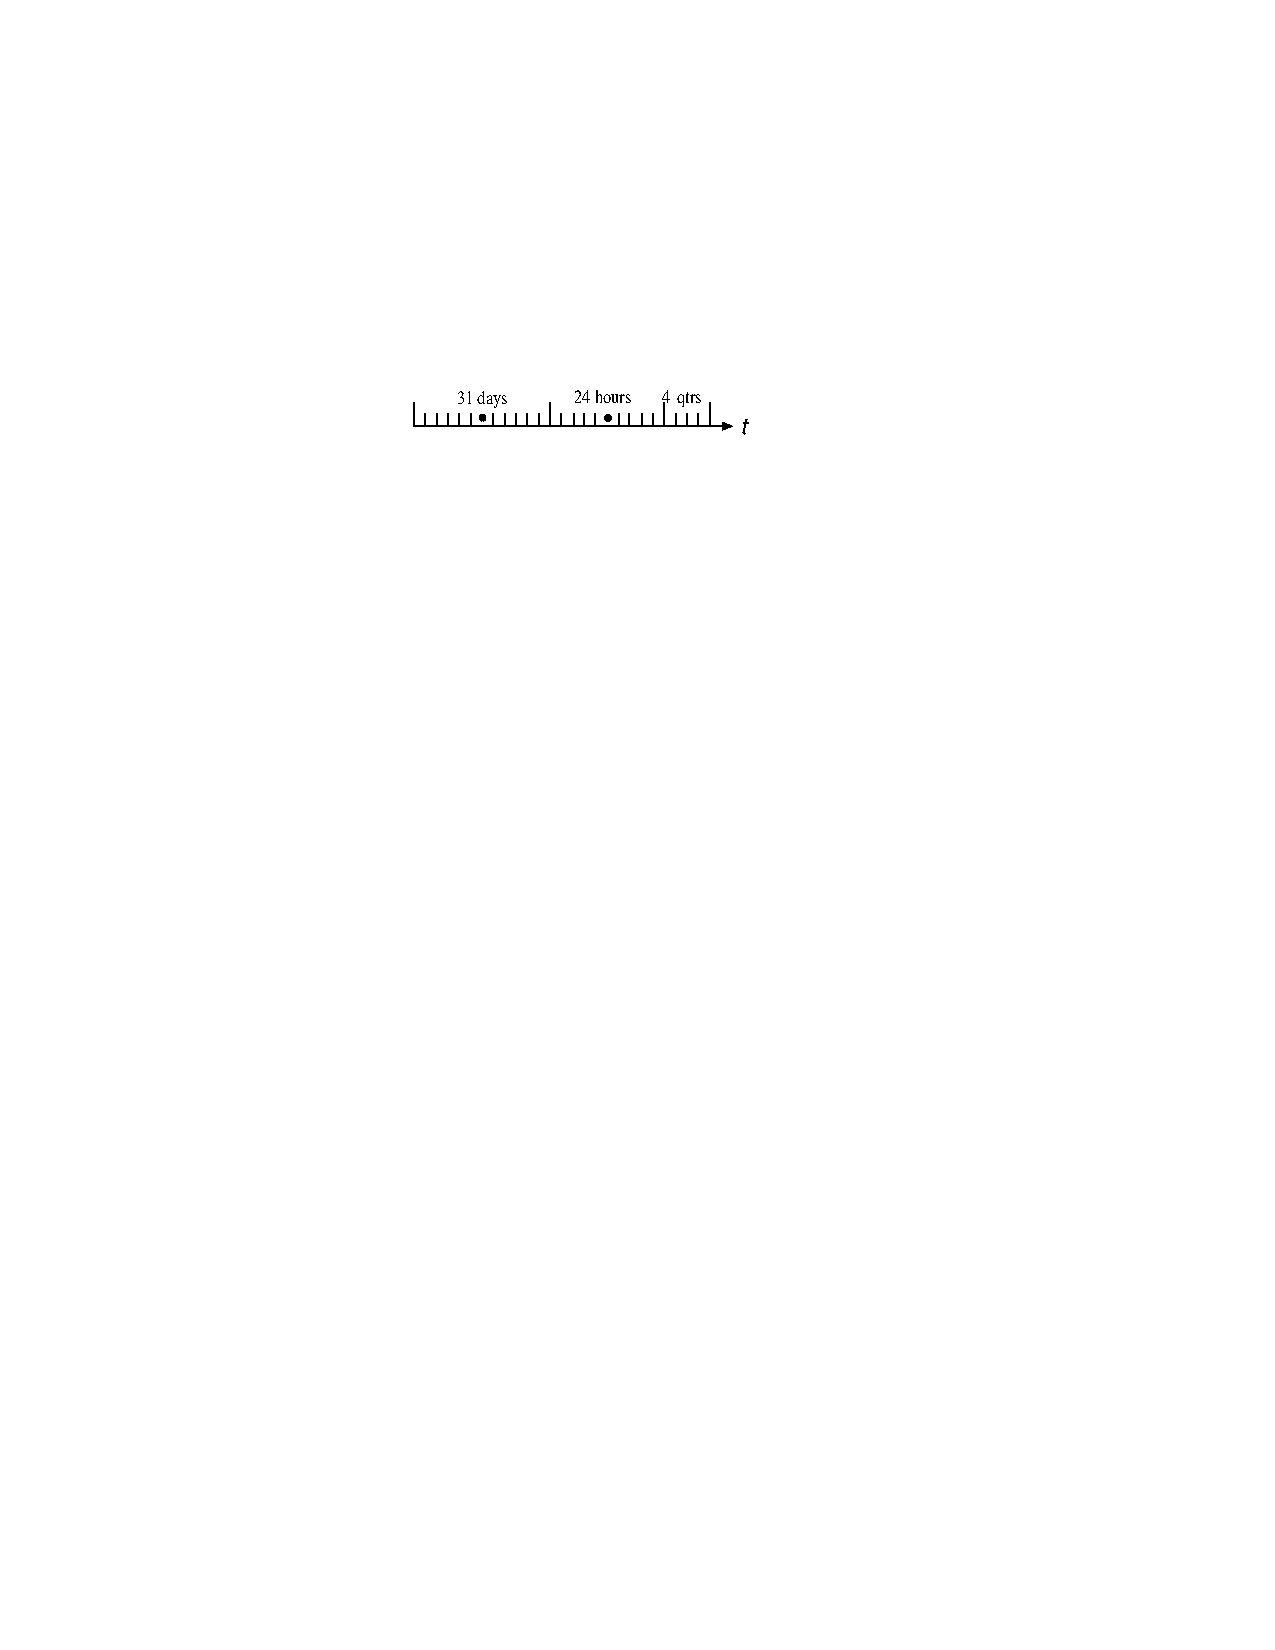
\includegraphics[width=3.0in]{figs/naturaltime.pdf}
        \caption{Natural Tilted Time Window}
        \label{fig:bg:ntime}
    \end{center}
\end{figure}
\paragraph{Natural Tilted Time Windowing:} In natural tilted time windowing, units of time is distributed non-uniformly. Most recent time gets more units. For example, Figure~\ref{fig:bg:ntime} shows a natural tilted time windowing scheme, where for most recent hour 4 units stores quarterly updates, 24 units of time storing a day, and 31 units storing a months summary. That is, with 59 units of time information, this model stores about 32 days' information.

\begin{figure}[htbp]
    \begin{center}
        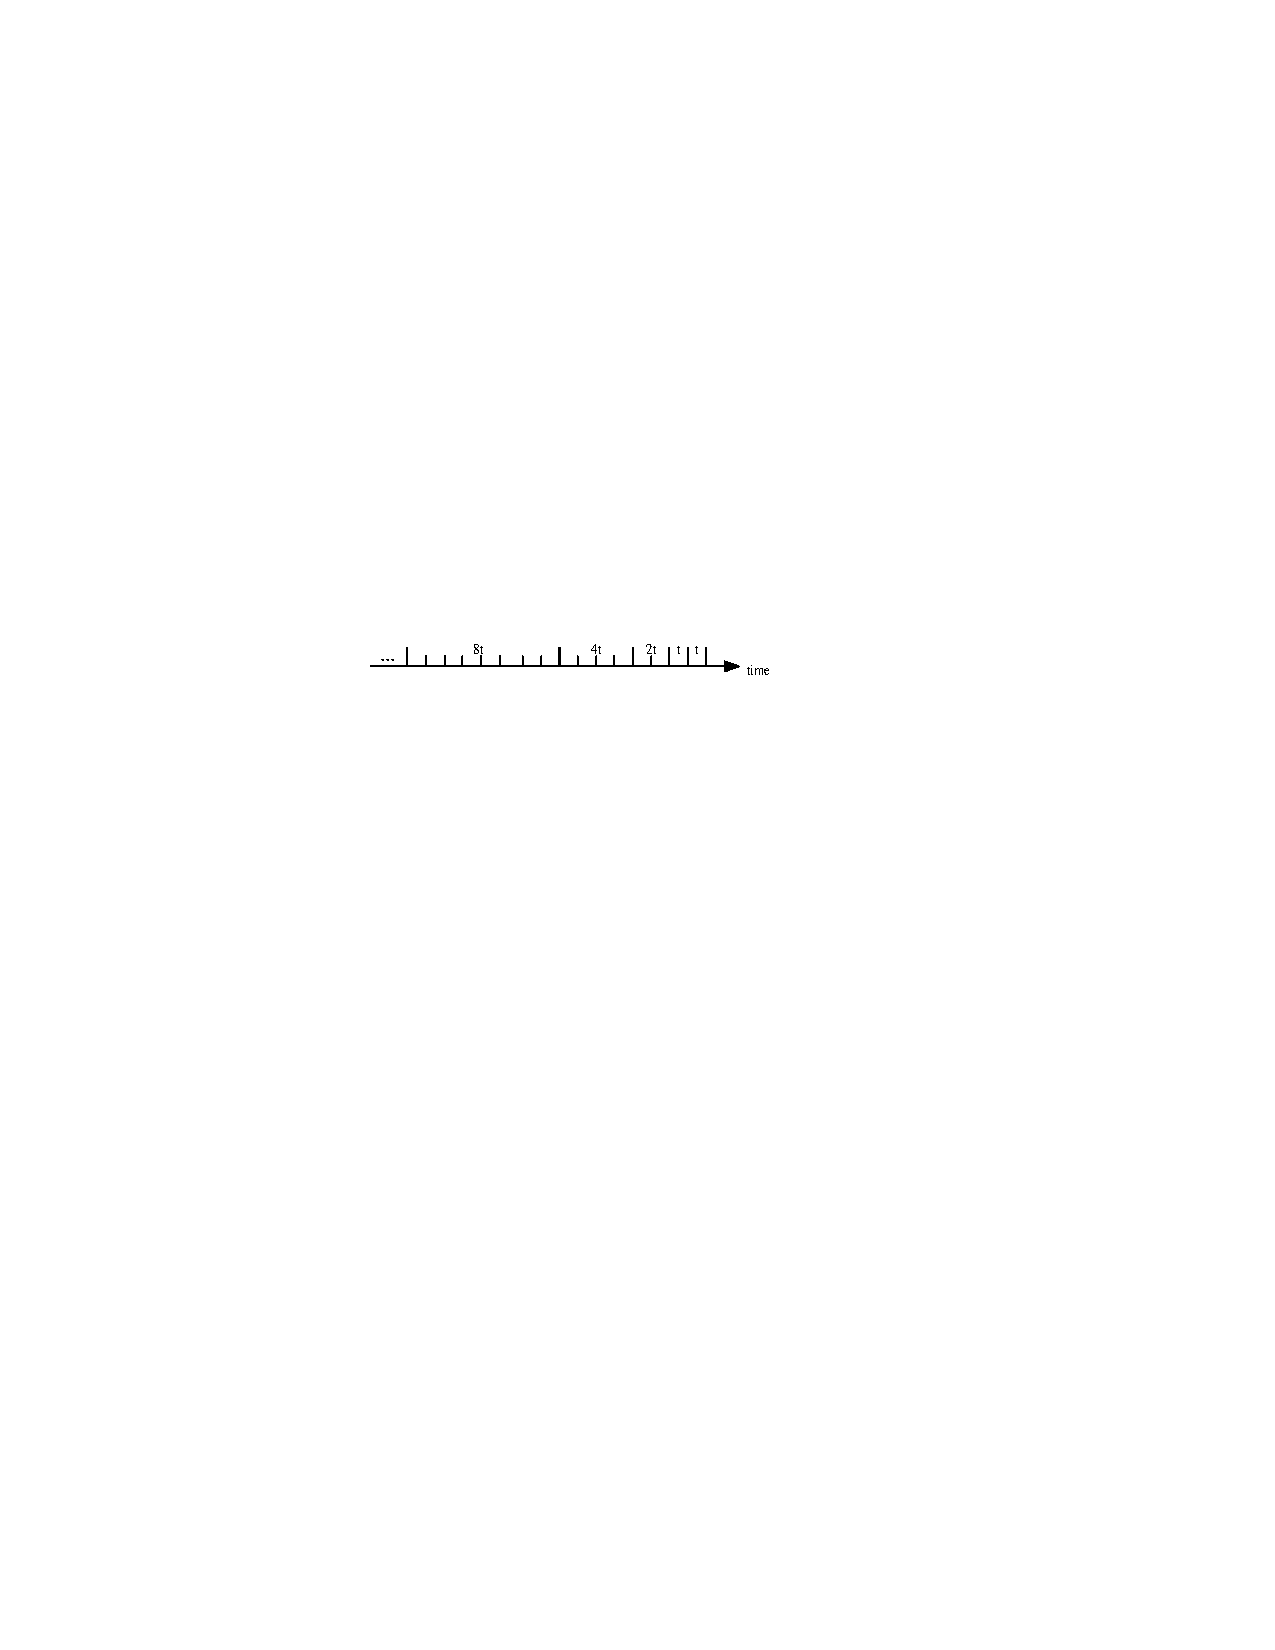
\includegraphics[width=4.0in]{figs/logtime.pdf}
        \caption{Logarithmic Tilted Time Window}
        \label{fig:bg:ltime}
    \end{center}
\end{figure}
\paragraph{Logarithmic Tilted Time Windowing:} Concept for logarithmic tilted time windowing is same as natural tilted time windowing. The only deference here is that time scale grows in logarithmic order. Figure~\ref{fig:bg:ltime} shows an example. 


\subsection{Change Detection}
\label{sec:bg:changedetection}
An assumption of most machine learning methods is that data is generated from a stationary distribution. As discussed in the previous section, this assumption does not hold for streaming scenario. Thus stream mining requires algorithms to facilitate drift detection methods. Differentiating between {\it noise} and {\it change} makes the problem challenging. The difference between a new distribution and noise is {\it persistence}, where new examples consistently follows new distribution rather than old. This section discusses several methods to detect and adapt learning algorithms in presence of concept drift.

\subsubsection{Detection}
Detection methods can generally be classified into two categories. First approach is to monitoring the evolution of various performance indicators as done in~\cite{klinkenberg98:changedetection, zeira04:changedetection}. Another approach is to maintaining two (or more) distributions varying the window length. Typically one window would summarize past history while the other would summarize most recent information~\cite{kifer04:condrift}.

Most methods follows the first approach. \cite{klinkenberg98:changedetection} monitors three performance indicators (accuracy, recall, and precision) over time, and uses their posterior comparison to a confident interval of standard sample errors for a moving average value for each indicator.

A classical algorithm for change detection is \textit{Cumulative Sum (CUSUM)}~\cite{page54:cusum}. CUSUM can detect that the mean of the input data is significantly different than zero. The test is as follows:
\[
    g_0 = 0 
\]\[
    g_t = max (0, g_{t-1} + (r_t - v))
\]
if $g_t > \lambda$ CUSUM triggers an alarm and set $g_t = 0$. This detects the changes in the positive direction, to detect the negative change $min$ is used instead of $max$. CUSUM does not require any memory. Its accuracy depends on the choice of $v$ and $\lambda$. Low $v$ results in faster detection with more false alarms.

For latter category, \cite{kifer04:condrift} uses Cherfnoff bound (Theorem~\ref{thm:chernoff}) and examines examples drawn from two probability distribution and decides whether these distributions are different.

\paragraph{ADWIN Algorithm:} ADWIN (ADaptive sliding WINdow) is another change detection algorithm of latter type. ADWIN keeps a variable length window of recent items. It ensures the property {\it there has been no change in the average value inside the window} for maximally statistically consistent length. The core idea of ADWIN is that whenever two {\it large enough} sub-windows of $W$ exhibit {\it distinct enough} averages, it is assumed that their corresponding expected values are different, and the older portion of the window is dropped. Essentially, this means that when the difference of means of the two windows is greater than a certain threshold $\epsilon_{cut}$, the older portion should be dropped. Equation to compute $\epsilon_{cut}$ is as follows:
\[
    m = \frac{2}{1/|W_0| + 1/|W_1|}
\]\[
    \epsilon_{cut} = \sqrt{\frac{1}{2m} \ln \frac{4 |W|}{\delta}}
\]
where $\delta \in (0, 1)$ is confidence value, an input.

\begin{algorithm}[htbp]
    \DontPrintSemicolon
\label{alg:adwin}
\caption{ADWIN Algorithm}

    \KwData{Data Stream}
    \KwResult{Window with most recent concept}
    \Begin{
        Initialize window $W$ \\
        \ForEach{$t > 0$} {
            $W \leftarrow W \cup \{x_t\}$ \tcp*[f]{add $x_t$ to the head of $W$ }\\
            \Repeat{$|\mu_{W_0} - \mu_{W_1}| < \epsilon_{cut}$ holds for every split of $W$} {
                Drop element from the tail of W\\
            }
            $W = W_0 . W_1$\\
        }
        Output $\mu_W$\\
    }
\end{algorithm}

ADWIN does not maintain the window explicitly, but compresses it using a variant of the exponential histogram technique. This means that it keeps a window of length $w$ using only $O(\lg w)$ memory and $O(\lg w)$ processing time per item.

\subsubsection{Adaptation to Change}
To improve accuracy of the decision model under concept drifting environment, decision model needs adaptation to the changes. There are two types of approaches based on when to adapt: 
\begin{itemize}    
    \item Blind or Periodic Methods: Models are updated on regular interval whether any change has actually occurred or not. 
    \item Informed Methods: Models are only updated when there are sufficient reasons to believe that changes in the concept have occurred.
\end{itemize}
It could be a good idea to use periodic methods where duration of seasonality is known beforehand. Otherwise, chosen duration could be too large or too small to response to the changes. In such cases, an informed decision is more desired. However, informed methods requires more resources (than blind methods) to be able to make such decision.

\subsection{Na\"ive Bayes Adaptation}
Naive Bayes algorithm is essentially a stream classification algorithm. One of the advantages of this classifier in the context of data stream is its low complexity for deployment. It only depends on the number of explanatory variables. Its memory consumption is also low since it requires only one conditional probability density estimation per variable.

\begin{algorithm}[htbp]
    \caption{VFDT: The Hoeffding Tree Algorithm}
    \label{alg:vfdt}
    \DontPrintSemicolon
    \SetKwInOut{Input}{Input} \SetKwInOut{Output}{Output} 
    
    \Input{$S$: Stream of examples \\
        $X$: Set of nominal attributes \\
        $Y$: Set of class labels $Y = \{y_1, y_2, \dots, y_k\}$ \\
        $G(.)$: Split evaluation function \\
        $N_{min}$: Minimum number of examples \\
        $\delta$: is one minus the desired probability \\
        $\tau$: Constant to resolve ties
    } 
    \Output{$HT$: is a decision tree}
    
    \Begin{
        Let $HT \leftarrow$ Empty Leaf (Root)
        \ForEach{$example(x, y_k) \in S$} {
            Traverse the tree $HT$ from root till a leaf $l$ \\
            
            \eIf (\tcp*[f]{Missing class label}) {$y_k == ?$ } {
                Classify with majority class in the leaf $l$
            } {
                Update sufficient statistics \\
                \If{$ Number\;of\;examples\;in\;l > N_{min}$ }{
                    Compute $G_l(X_i)$ for all attributes \\
                    Let $X_a$ be the attribute with highest $G_l$ \\
                    Let $X_b$ be the attribute with second highest $G_l$ \\
                    Compute $\epsilon = \sqrt{\frac{R^2 \ln(2/\delta)}{2n}}$  \tcp*[f]{Hoeffding bound} \\
                    
                    \If{$G(X_a) - G(X_b) > \epsilon\; || \;\epsilon < \tau$} {
                        Replace $l$ with a splitting test based on attribute $X_a$ \\
                        Add a new empty leaf for each branch of the split \\
                    }
                }
            }
        }
        Return $HT$
    }

\end{algorithm}

\subsection{Very Fast Decision Tree}
\label{sec:bg:vfdt}
Very Fast Decision Tree (VFDT), also known as Hoeffding Tree (HT), is the stream adaptation of decision tree generating from a stationary distribution. It is an anytime-ready algorithm and uses Hoeffding bounds to ensure the performance in terms of accuracy is asymptotically nearly identical to that of conventional tree algorithms. VFDT runs on constant time and memory per examples and can serve thousands of examples on a typical consumer system.

VFDT constructs the tree by recursively replacing leaves with decision nodes. Each leave stores sufficient statistics that are used to evaluate the merit of split-test and to decide the target class. For incoming instances, the tree is traversed from the root to a leaf (based on the incoming instance's values) and the statistics are updated accordingly. If a unanimous decision cannot be reached based on observed instances at that particular leaf node, the node is tested to check the sufficiency for a split. If there is enough statistical support in favor of split, the node is splitted on the best attribute and stats are passed to the descendants (new leaves). Number of descendants of this new decision node is equal to the number of possible values of the chosen attribute. Thus, the tree is not necessarily a binary tree.

Deciding on whether to split a node or not is a unique contribution of VFDT. VFDT solves this difficult problem of deciding exactly how many examples are required to be observed by a leaf node before splitting by using Hoeffding bound (Theorem~\ref{thm:hoeffding}). Consider $G(.)$ be the heuristic measure of the attributes. This measure could be information gain as of C4.5 or Gini index of CART. For information gain range $R$ in Hoeffding bound is $\lg (\#classes)$. Goal is to find $n$ such that the attribute chosen for split after observing $n$ instances, would, with high probability, be the same as it would be chosen after observing infinite instances. Assume that $X_a$ is the attribute with the best $G(.)$, and $X_b$ is the second best attribute after observing $n$ instances. Then $\Delta G = G(X_a) - G(X_b)$ be the difference between their observed heuristics. From Hoeffding bound, we know if $\Delta G < \epsilon$, then with probability $1 - \delta$ $X_a$ would be the attribute with highest value in the evaluation function in the universe. Otherwise, if $\Delta G < \epsilon$, then the sample size is not enough to make a stable split decision. As the assumption is that underlying generating distribution is stationary, thus as the sample size increases, $\epsilon$ decreases and heuristic value for most informative attribute goes up.

To fasten up the process, VFDT uses an extra parameter $N_{min}$ to reduce the number of $G(.)$ computation. Computing $G(.)$ when there are too few instances is run-time inefficient. Thus a user parameter $N_{min}$ is used to indicate minimum number of instances needed to be observed before the evaluation starts.

When multiple attributes continuously perform similar in heuristic evaluation after observing a large number of examples, $\Delta G$ might never be greater than $\epsilon$. To break such tied cases, another user parameter $tau$ is used, and when $\epsilon$ falls below $\tau$ (i.e. $\Delta G < \epsilon <\tau$), algorithm splits on the best attribute. Algorithm~\ref{alg:vfdt} summarizes the pseudo-code of VFDT.

There are some property of VFDT that are different than C4.5. In contrast to the C4.5 algorithm number of examples that support a decision increases in VFDT. Typically VFDT also results a low variance model than that of C4.5. However, there is no mechanism avoid over-fitting in VFDT as there is no room for pruning.

\begin{algorithm}[htbp]
    \DontPrintSemicolon
    \SetKwInOut{Input}{Input} \SetKwInOut{Output}{Output} 
    \caption{CVFDT: Concept-adapting VFDT}
    \label{alg:cvfdt}
    
    \Input{$S$: Stream of examples \\
        $X$: Set of nominal attributes \\
        $Y$: Set of class labels $Y = \{y_1, y_2, \dots, y_k\}$ \\
        $G(.)$: Split evaluation function \\
        %$N_{min}$: Minimum number of examples \\
        $\delta$: is one minus the desired probability \\
        $\tau$: Constant to resolve ties \\
        $w$: Size of the window \\
        $n_{min}$: Number of examples between checks for growth \\
        $f$: Number of examples between checks for drift
    } 
    \Output{$HT$: is a decision tree}
    
    \Begin{
        Let $HT \leftarrow$ Empty Leaf (Root) $l_0$ \\
        Let $Alt(l_0) \leftarrow \emptyset$ \tcp*[f]{Alternate trees for $l_0$} \\
        %Let $G(X_\emptyset)$ be the $G(.)$ obtained by predicting most frequent class \\
        %Let $X_1 = X \cup \{X_\emptyset\}$ \\
        
        \ForEach{class $y_k$} {
            \ForEach{$x_{ij} \in X_i \in X$} {
                Set $n_{ijk} = 0$
            }
        }
        \ForEach{$example(x, y) \in S$} {
            Traverse the tree $HT$ including $Alt(\{n: (x,y)\;passes\;through\;n\;in\;HT\})$ trees root till a set of leaves $L$ \\
            
            Set $id = \max(\{L.id\})$ \\
            Add $((x, y), id)$ to the beginning of $W$ \\
            \If{$|W| > w$} {
                Let $((x_w, y_w), id_w)$ be the last element in $W$ \\
                FORGET($HT, n, (x_w, y_w), id_w)$) \label{algln:cvfdt:forget} \\
                $W = W - ((x_w, y_w), id_w)$
            }
            GROW($HT, n, G, (x,y)$ \\
            \If{examples seen since last checking $> f$}{
                VALIDATE\_SPLIT($n$) \label{algln:cvfdt:validatesplit} 
            }
        }
        Return $HT$
    }
\end{algorithm}
\subsection{Concept-adapting Very Fast Decision Tree}
Concept-adapting Very Fast Decision Tree (CVFDT) is the extension of CFDT that adds the ability to adapt the model by detecting the changes in the underlying distribution that generates the examples. CVFDT does not require the model to be recomputed, instead it updates the sufficient statistics stored in each node that the new instances affects by maintaining a sliding window. It increases the counter of new instances and decreases count of oldest examples which now need to be forgotten. If the underlying distribution is stationary, this would not have any effect. But in case of a concept drifting distribution, some decision nodes that previously had passed the Hoeffding bound test will no longer pass, rather an alternate attribute would now have higher or similar gain. CVFDT keeps stats to detect such situation and starts maintaining an alternate subtree with the new best attribute as its root. When this alternate subtree becomes more accurate on new data then the old subtree is replaced by the new one. Pseudo-code of CVFDT has be shown in Algorithm~\ref{alg:cvfdt}. The sub-routine $GROW$ is essentially the Hoeffding Tree algorithm where instead of only keeping stats in the leave, every node keeps track of the instances it has seen. Two other sub-routines $FORGET$ and $VALIDATE\_SPLIT$ have been shown separately.

\begin{algorithm}[htbp]
    \ContinuedFloat
    \DontPrintSemicolon
    \LinesNumberedHidden
    \setcounter{algoline}{0}
    \newcommand\Numberline{\refstepcounter{algoline}\nlset{\thealgoline}}
    \SetNlSty{textbf}{\ref*{algln:cvfdt:forget}.}{}
    
    \SetKwInOut{Input}{Input} \SetKwInOut{Output}{Output} 
    \SetKwInOut{TitleOfAlgo}{Algorithm}
    \TitleOfAlgo {FORGET($HT, n, (x_w, y_w), id_w$)}
    \label{alg:cvfdt:forget}
    
    \Begin{
        \Numberline Sort $(x_w, y_w)$ through $HT$ while it traverses leaves with $id \le id_w$ \\
        \Numberline Let $P$ is the set of sorted nodes \\
        
        \Numberline \ForEach{node $l \in P$} {
        \Numberline     \ForEach{$x_{ij} \in x : X_i \in X_l$} {
        \Numberline         Decrement $n_{ijk}(l)$
            }
        \Numberline     \ForEach{tree $t_{alt} \in Alt(l)$} {
        \Numberline         FORGET($t_{alt}, n, (x_w, y_w), id_w$)
            }
        }
    }
\end{algorithm}

$FORGET$ function is used to remove the effect of instances of older concepts. However, this is not straight-forward as HTs go through changes after the instance to be forgotten was initially added. Thus, CVFDT uses monotonically increasing ids for the nodes. When a new instance is added to the window ($W$), the maximum $Id$ of the leaves it reaches in $HT$ and all the alternate trees is recorded with it. To remove the effect of a old instance, counts are decremented at every node the example reaches in $HT$ whose $Id$ is less than the stored $Id$.

\begin{algorithm}[htbp]
    \ContinuedFloat
    \DontPrintSemicolon
    \LinesNumberedHidden
    \setcounter{algoline}{0}
    \newcommand\Numberline{\refstepcounter{algoline}\nlset{\thealgoline}}
    \SetNlSty{textbf}{\ref*{algln:cvfdt:validatesplit}.}{}
    
    \SetKwInOut{Input}{Input} \SetKwInOut{Output}{Output} 
    \SetKwInOut{TitleOfAlgo}{Algorithm}
    \TitleOfAlgo {VALIDATE\_SPLIT($HT, n, (x_w, y_w), id_w$)}
    \label{alg:cvfdt:validatesplit}
    
    
    \Begin{
        \Numberline Let $HT \leftarrow$ Empty Leaf (Root) $l_0$ \\
        \Numberline Let $Alt(l_0) \leftarrow \emptyset$ \tcp*[f]{Alternate trees for $l_0$} \\
        
        \Numberline \ForEach{internal node $l$ in $HT$} {
        \Numberline     \ForEach{$t_{alt} \in Alt(l)$} {
        \Numberline         VALIDATE\_SPLIT($t_{alt}, n, (x_w, y_w), id_w$)
                    }
        \Numberline     \ForEach{$x_{ij} \in X_i \in X$} {
        \Numberline         Set $n_{ijk} = 0$
                        }
                    }
        \Numberline Let $X_a$ be the current split attribute \\
        \Numberline Compute $\Delta(G) = G_l(X_n) - G_l(X_b)$  \tcp*[f]{$X_n, X_b$ two current highest 		attributes} \\
        
        \Numberline \If{$\Delta(G) \ge 0 \&\& X_n \not\in \{roots of Alt(l)\}$ } {
        \Numberline     Compute $\epsilon = \sqrt{\frac{R^2 \ln(2/\delta)}{2n}}$  \tcp*[f]{Hoeffding bound} \\
        \Numberline     \If{$\Delta(G) > \epsilon\; || \;\epsilon < \tau \&\& \Delta(G) \ge \tau/2$} {
        \Numberline         Let $l_{new}$ be an internal node that splits on $X_n$ \\
        \Numberline         $Alt(l) = Alt(l) + l_{new}$ \\
        \Numberline         \ForEach{branch of the split} {
        \Numberline             Add a new leaf $l_m$ to $l_new$ \\
        \Numberline             $X_m = X - {X_n}$ \\
        \Numberline             $Alt(l_m) = {}$ \\
                    
        \Numberline             Compute $G_m(X_\emptyset)$ using most frequent class at $l_m$ \\
        \Numberline             \ForEach{node $l \in P$} {
        \Numberline                 \ForEach{$x_{ij} \in x : X_i \in X_l$} {
        \Numberline                     Decrement $n_{ijk}(l)$
                        }
                    }
                }
            }
        }
    }
\end{algorithm}

Lastly, there is $VALIDATE\_SPLIT$ sub-routine that periodically checks the internal nodes of $HT$ where current split attribute would no longer have the highest $G(.)$ or $\Delta G$ would be less than $\epsilon$ or $\Delta G$ would be less than $\tau/2$. This is similar condition as to the original one with more restrictive tie condition. The added restriction ensures less alternate tree creation.

Now that related concept of basic learning algorithms and stream mining are discussed, in the next section, the concepts of ensemble learning are presented.

\section{Ensemble Learning}
Ensemble learning, due to its intrinsic merits, focuses to get the best out of a collection of base learners. Ensemble learning can be thought of as a divide-and-conquer approach. However, it may not necessarily divide the tasks rather might do more tasks. The motivation behind was presented in the previous chapter. In short, ensemble methods are interesting because of following possibilities:
\begin{itemize}
    \item Avoiding worst classifier by averaging several classifier.
    \item Fusing multiple classifier to improve performance of the best classifier.
    \item Arranging the better classifiers (might include the best one) in a way to outperform the best one.
    \item Dividing streams into chunks, learn separate models from each and then combine their results (divide and conquer).
\end{itemize}

A number of methods have been developed in past couple of decades focusing on these motivations. They employ different approaches to improve the final classifier. Following is a summary of different approaches of generating ensembles of classifiers.
\begin{itemize}
    \item Creating multiple training sets by resampling the original set and feeding those into different learners.
    \item Using different combination of features to learn multiple classifiers.
    \item Manipulating class labels. For example, transforming the classes into binary classification problem by partitioning the class labels into disjoint subsets.
    \item Manipulating the learning algorithms such that they result different outcomes for the same training set. For example, introducing certain randomness into tree growing algorithm.
\end{itemize}

In this section, we present these basic concepts of building an ensemble of a collection of classifier. We start with primitive methods such as bagging and boosting. However, we are particularly interested in more sophisticated methods based on decision tree learning methods of stream data such as Adaptive Size Hoeffding Tree (ASHT) and ADaptive WINdow bagging (ADWIN bagging).

\subsection{Bagging}
\label{sec:bg:bagging}
Bagging, also known as bootstrap aggregating, is a meta algorithm that improves accuracy and reduces variance and chance of over-fitting. Bagging is typically used with tree based learners. Given a training set $D$ of size $n$, bagging generates $m$ new training sets $D_i$ of size $n_{new}$ where $i = \{1, 2, \dots, m\}$ by sampling with replacement. If $n = n_{new}$ approximately two-thirds of the instances of $D_i$ is expected to be unique examples of $D$ while rest being duplicates. If $K$ is the number of examples belonging from the original training set then $P(K=k) = \binom{n}{k} \left( \frac{1}{n}\right)^k \left(1- \frac{1}{n}\right)^{n-k}$. These $m$ sets are then used to learn $m$ classifier. Final decision is given by a majority voting scheme over the decision of these $m$ classifiers. Figure~\ref{fig:bg:bagging} shows an illustrative example of bagging method.
\begin{figure}[htbp]
    \begin{center}
        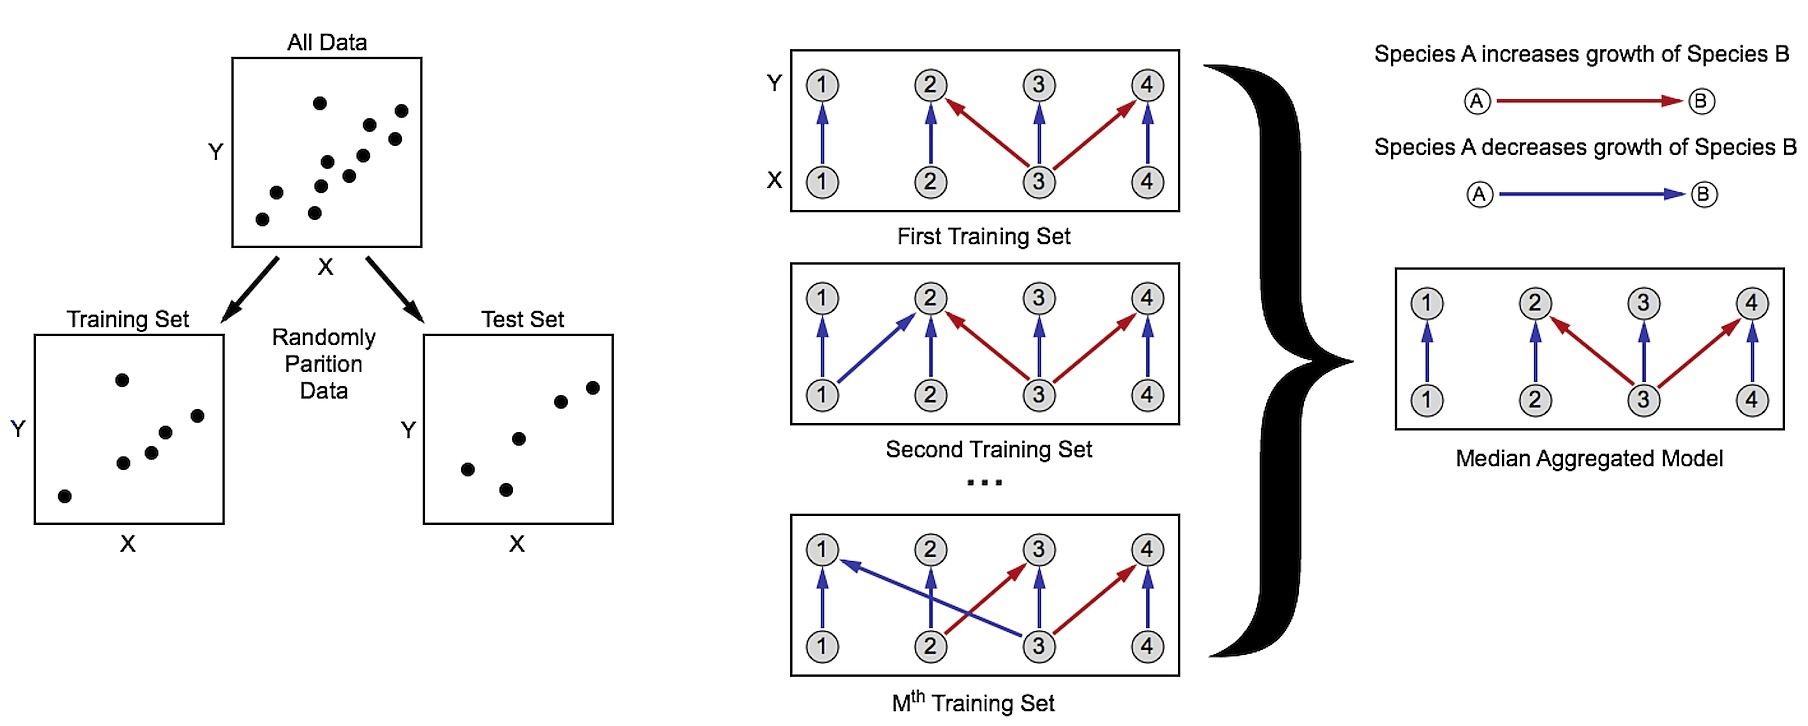
\includegraphics[width=10.0cm]{figs/bagging.jpg}
        \caption{Bagging or bootstrap aggregation}
        \label{fig:bg:bagging}
    \end{center}
\end{figure}

For online bagging approach $n \rightarrow \infty$, and the Binomial distribution of $P(K=k)$ tends to a Poisson distribution with $P(K=k) = \exp(-1)/k!$. Using this justification, online bagging chooses a $k ~ Poisson(1)$ for each incoming training examples $(x_i, y_i)$, and updates the base learning learning algorithms $k$ times. The classification is done as the same way of batched approach, by unweighted voting of $m$ base classifiers. For similar distribution of training examples, online bagging produces similar approximated base models. If (i) used based learner converges to the same same classifier with increasing training examples, and (ii) base learner produces same classifier given a fixed training set for both batched and online bagging methods; then online bagging will converge to the classifier obtained though batched learning methods.


\subsection{Boosting}
Boosting is another supervised learning algorithm to iteratively improve learning hypothesis. The motivation behind the boosting approach is that a set of weak classifier could create a single strong learner. It forces a weak classifier to update or generate new rules that make less mistakes on previously misclassified records. Initially all records are assigned same weights. At the end of a boosting round, weights might change due to the errors in classification. Weights of the instances are increased or decreased if they are classified wrongly or correctly, respectively. Thus successive classifiers depend upon their predecessors. 
\begin{figure}[htbp]
    \begin{center}
        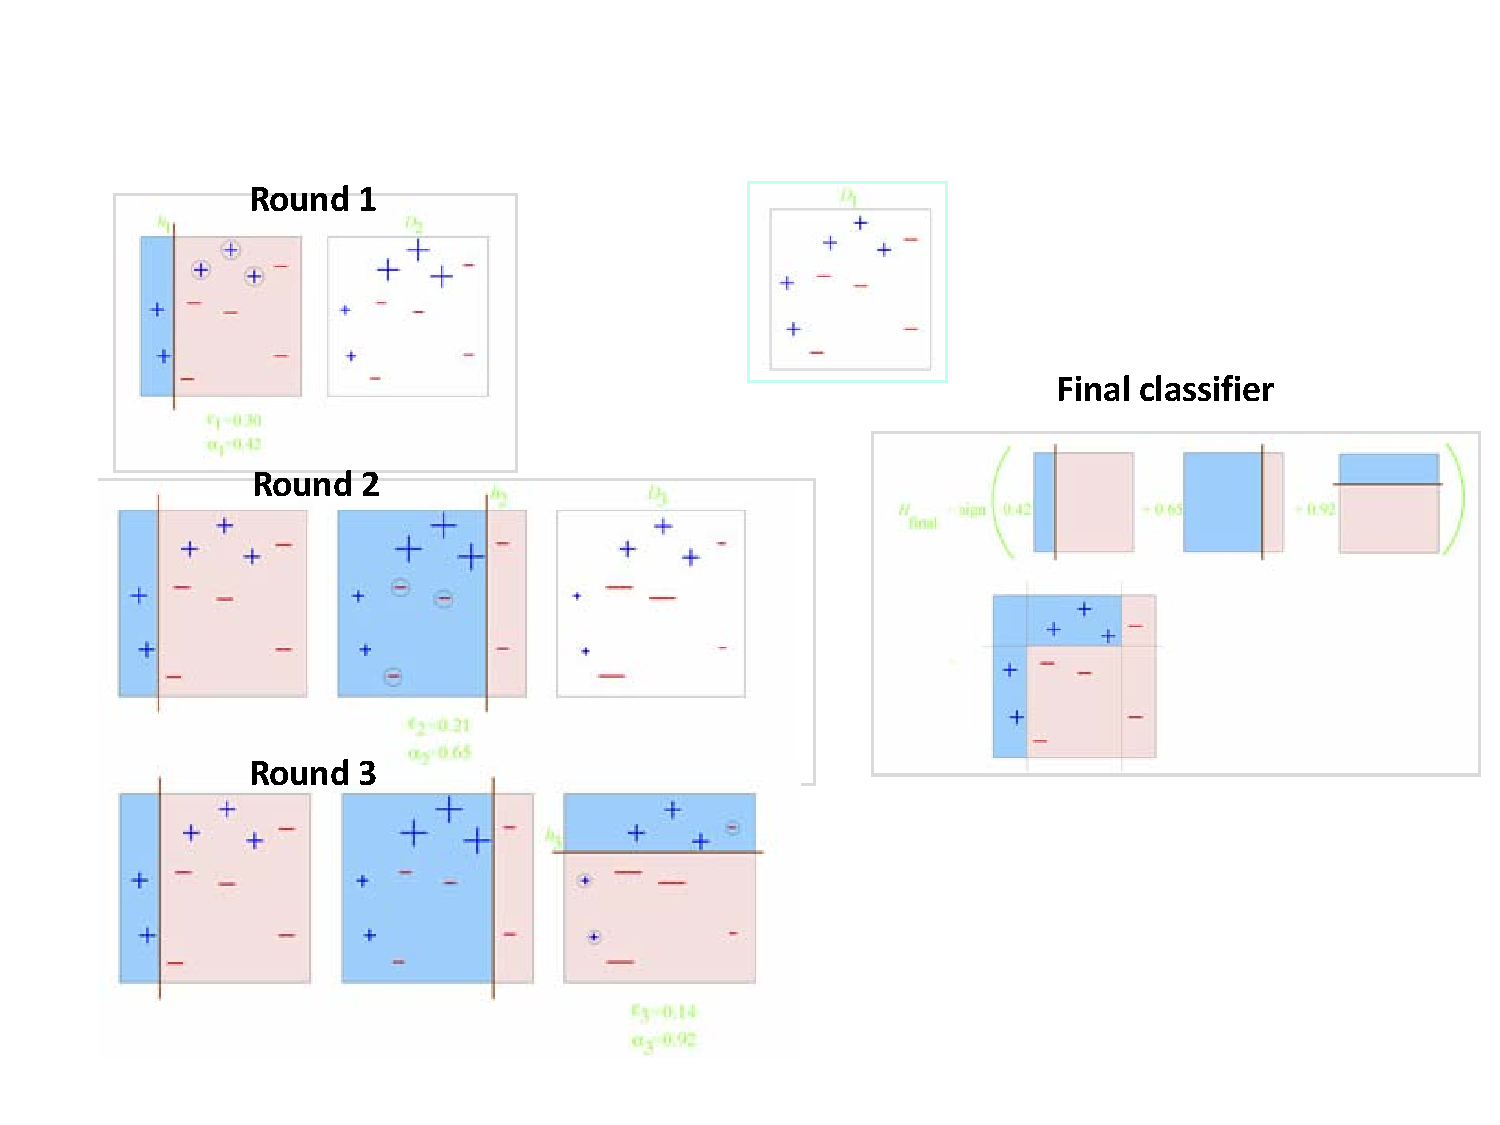
\includegraphics[width=10.0cm]{figs/boosting.pdf}
        \caption{Boosting method example}
        \label{fig:bg:bagging}
    \end{center}
\end{figure}

Mathematically, let $H= \{h_1, h_2, \dots, h_n\}$ be $n$ weak hypotheses. The combined hypothesis $H(.)$ is a weighted majority vote of the $n$ weak hypotheses where each hypothesis $h_i$ has a weight of $\alpha_i$ for $i = \{1, 2, \dots, n\}$:
\begin{equation}
\label{eqn:adaboostHypo}
    H(.) = sign \left(\sum_{i=1}^n \alpha_i h_i(x) \right).
\end{equation}

One of the earliest boosting approach was proposed in~\cite{schapire90:whyens}. It calls weak learners three times on three modified distributions and achieves slight improvement in accuracy. Later,~\cite{freund97:boosting} proposed AdaBoost, an adaptive boosting method, that works with a principle of minimizing upper bound of empirical error. Let, $(x_1, y_1), (x_2, y_2), \dots, (x_n, y_n)$ are given examples where $x_i \in X, y_i \in Y = [-1, +1]$. Let, $D_t (i)$ be the weight of $i$-th example at $t$-th round. Then, AdaBoost initializes $D_1(i) =1/n$. Iterative steps are as follows:

For each iteration $t= 1, 2, \dots, T$:
\begin{itemize}
    \item Train weak learner using distribution $D_t$
    \item Get weak hypothesis $h_t : X \rightarrow \{-1, +1\}$ with error
    \[
        \epsilon_t = Pr_{i ~ D_t} [h_t(x_i) \ne y_i]
    \]
    \item Choose $\alpha_t = \frac{1}{2} \ln \left( \frac{1 - \epsilon_t}{\epsilon_t} \right)$
    \item Update $D_{t+1} (i) = \frac{D_t(i) \exp(-\alpha y_i h_t(x_i))}{Z_t}$ where $Z_t$ is a normalization factor
\end{itemize}
Finally, the output is calculated with the Equation~\ref{eqn:adaboostHypo} given above.

An online variant of AdaBoost uses a similar approach as online bagging method, simulating sampling with replacement using Poisson distribution. However, the Poisson parameter $\lambda$ (Equation~\ref{eqn:poisson}) associated with an example is increased if that particular example is misclassified. In case of correct classification $\lambda$ is decreased. Similar to the AdaBoost, online boosting approach assigns total weights equally to the correctly and misclassified instances, i.e. half of the total weights each. Unlike AdaBoost, in online boosting weights are updated based on only the examples seen thus far rather than the complete training set. This is intuitively problematic as initial hypotheses are build on too few examples. Even with this limitation, online boosting shows good performance. Online boosting with naive Bayes base learner converges to the model achieved with AdaBoost as the number of training instances tends to infinity.

\subsection{Adaptive-Size Hoeffding Tree (ASHT) Bagging}
In previous section (Section~\ref{sec:bg:vfdt}), we have introduced Very Fast Decision Tree (VFDT) or Hoeffding Tree (HT). Hoeffding Tree is inspired by the fact that a small sample size could be enough to effectively choose an optimal splitting attribute. An upper bound of the error introduced because of such generalization is given using Hoeffding bound.

The Adaptive-Size Hoeffding Tree (ASHT) is, as the name suggests, extended from Hoeffding tree with deletion of nodes or reseting of the tree capabilities. Following are two significant differences of adaptive-size Hoeffding tree with Hoeffding tree: 
\begin{itemize}
    \item Maximum number of split nodes or the size of the tree is bounded in ASHT. There is no such limit on HT. HT grows indefinitely as the data and new concepts are introduced.
    \item When number of split nodes exceeds the maximum value (essentially after a new split), some nodes are deleted to retain the tree property (max size).
\end{itemize}
There are two different choices for the deletion of nodes for the second point. First option is to delete the oldest node. In Hoeffding tree, root is always the oldest node. All children of root except for the nodes that were further splitted are also deleted in this case. The new root would be the root of the child not being deleted. Another and more crude approach would be to delete the complete altogether i.e. reseting the tree. 

\begin{figure}[htbp]
    \begin{center}
        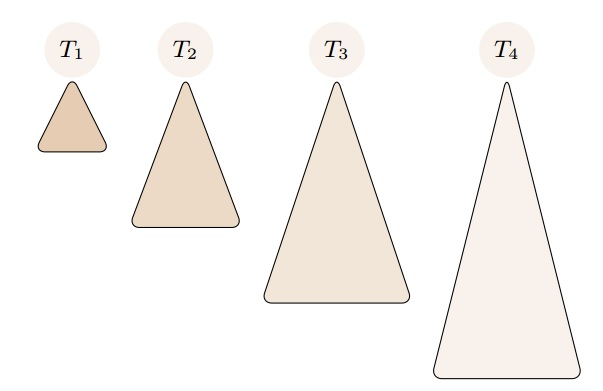
\includegraphics[width=10.0cm]{figs/asht.jpg}
        \caption{Adaptive Size Hoeffding Tree concept}
        \label{fig:bg:asht}
    \end{center}
\end{figure}

Based on this modified Hoeffding tree, a bagging method is developed in~\cite{bifet09:asht}. The intuition of the methods is as follows: smaller trees adapts to changes faster than the larger trees. However, larger trees perform better where data has only small changes or drifts because of the fact the it is built with more data. A tree of size $s$ would expected to be reset twice as often as a tree with size $2s$. Using an ensemble of different sizes would thus give a set of trees with different reset speeds. Smaller trees would be updated for smalls changes in the streams, while larger ones will maintain a history for longer period. Polling over this set of classifier would thus expected to result in a classifier with finer granularity. It is to be noted that reset will occur even for stationary data, however, this should not have any negative influence on the ensemble's predictive performance for stationary cases.

The proposed bagging method in~\cite{bifet09:asht} uses $n$ adaptive-size Hoeffding trees. The $n$-th ASHT has twice the maximum size of $(n-1)$-th tree. Size of the smallest tree is 2. For the polling, each tree is associate with a weight, which is selected to be the inverse of squared error.

\subsection{ADWIN Bagging}
ADWIN Bagging combines three different powerful concepts together: (i) bagging (Section~\ref{sec:bg:bagging}), (ii) adaptive window change detection (Section~\ref{sec:bg:changedetection}), and (iii) Hoeffding tree (Section~\ref{sec:bg:vfdt}).

Bagging using ADWIN is implemented as ADWIN Bagging where the Bagging method is the online bagging method of Oza and Rusell~\cite{oza01:obagboost} with the addition of the ADWIN algorithm as a change detector. Hoeffding Trees are used as base classifier. When a change is detected, the worst classifier of the ensemble of classifiers is removed and a new classifier is added to the ensemble. 

\chapter{Data Set Generation}
\label{chp:dataset}
Due to the lack of labeled real-world data streams, stream mining algorithms are usually tested with synthesized data. Synthesized data has several advantages over poorly labeled real-world data streams. First of all, it is rather easy to produce. It has significantly less storage overhead. It is easier to control synthesizing parameters to generate data sets with the desired concept drift, recurrence, etc. scenarios.

In this chapter, we briefly discuss some of these generators. For our experimentations we used the random radial basis function (RBF) generator. Thus, we  discuss the generation process and the generated stream's properties from a random RBF generator in greater details. We then describe the modifications in the generation process to introduce variable speed RBF streams.

\section{Existing Stream Generators}
A number of generators have been introduced in literature in the past decades: SEA concept generator, STAGGER concepts generator, rotating hyperplane generator, random RBF generator, waveform generator are some of the commonly used ones. 

\subsection*{SEA Concepts Generator}
The SEA concept generator is introduced in~\cite{street01:sea} to generate a synthetic data set with abrupt concept drift. It uses three parameters valued between $0$ and $10$ inclusive. The points of the data set are divided into blocks of different concepts. Classification within each block is controlled using the input parameters along with a threshold value.

\subsection*{STAGGER Concepts Generator}
STAGGER is one of the early methods developed for stream generation~\cite{schlimmer86:stagger}. Binary concepts are generated from three attributes: size, shape, and color. Each of the attributes has three possible values: small, medium, and large are the sizes; circle, triangle, and rectangle are the shapes; and red, blue, and green are the colors. The total $27$ combinations are being mapped into a binary class by this generator.

\subsection*{Rotating Hyperplane Generator}
A rotating hyperplane generator is introduced in the evaluation of CVFDT~\cite{hulten01:cvfdt}. Hyperplanes can effectively be used to simulate concept drifting environments. A hyperplane in a $d$-dimensional space is a set of points $x$ that satisfies the following equation:
\[
    \sum_{i=1}^{d} w_i x_i = w_0 = \sum_{i=1}^{d} w_i
\]
where $x_i$ is the $i^{th}$ coordinate of $x$. The hyperplane works as the boundary between two of the binary classes. By controlling the orientation and position of the hyperplane concept drift can be controlled. 

\subsection*{Wavefront Generator}
The wavefront generator is a data set available at the UCI machine learning repository~\cite{internet:ucirepo}. Two or three base waves are used to generate a data set of three different classes of waveforms. The prediction task is to predict the classes of waveforms. The optimal Bayes classification rate is known to be $86\%$. There are two variations of this generator: wave21 and wave40. Wave21 uses 21 numeric noisy attributes, and wave40 uses 19 more irrelevant attributes along with original 21.

\subsection*{LED Generator}
LED generator is also available at the UCI machine learning repository~\cite{internet:ucirepo}. The prediction task for this data set is to predict the digit displayed on a seven segment LED display. Each segment has $10\%$ chance of being inverted. The optimal classification using na\"ive Bayes on this data set is  $74\%$. 

\subsection*{Random Radial Basis Function Generator}
All the generators mentioned above are relatively simple and easy to use. However, it is harder to model a complex scenario with those generators. Hypothesis spaces for these generators are not very large, except for the rotating hyperplane generator. But with the rotating hyperplane generator it is harder to produce overlapping space and outliers. A random radial basis function (RBF) generator is therefore introduced to generate a complex concept type that is not straightforward to approximate, especially with a decision tree model.

\begin{figure}[htbp] 
    \begin{center}
        \begin{tabular}{cc}
            \hspace{-5mm}\resizebox{90mm}{!}{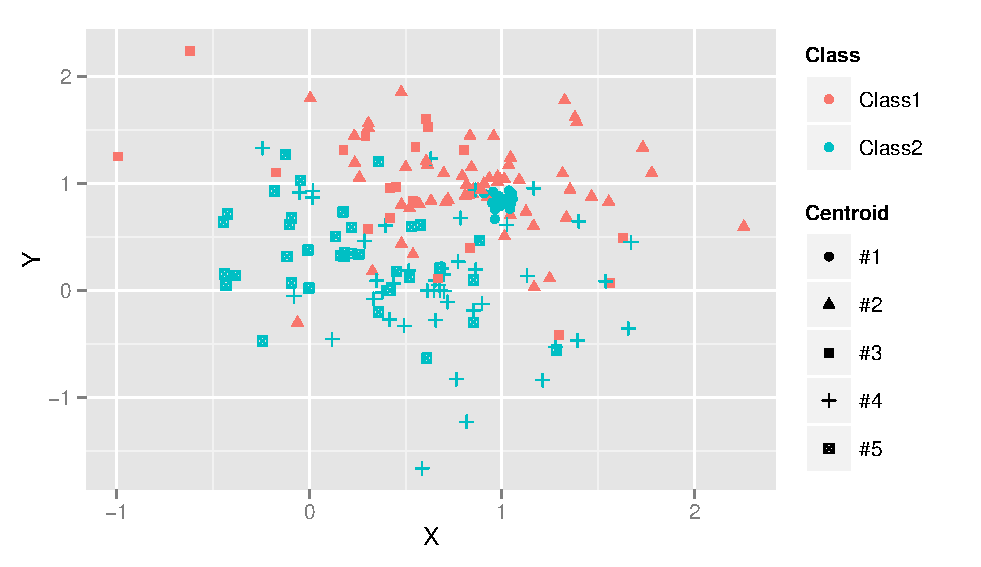
\includegraphics{figs/rbf5x2.pdf}} &
            \hspace{-10mm}
            \resizebox{70mm}{!}{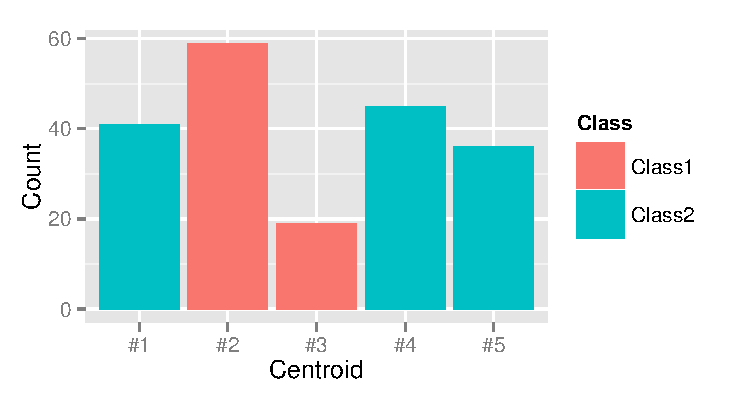
\includegraphics{figs/rbf5x2-hist.pdf}} \\
            \scriptsize{(a)\vspace{2mm}} &
            \scriptsize{(b)}    
        \end{tabular}
        \caption{RBF data generation with 5 centroids in 2D space (a) distribution (b) histogram}
        \label{fig:ds:rbf}
    \end{center}
\end{figure}

The RBF generator starts by selecting a fixed number of random centroids, each at a random position in the hyperspace with a random standard deviation, class label and weight. Instances are generated by selecting a centroid at random and generating a random point near that centroid by maintaining a Gaussian distribution with the previously selected standard deviation and the location of the centroid as mean. The probability of selecting any centroid is proportional to its weight. Direction of the deviation is selected at random. The class label of the instance is assigned to be the one of the selected centroid. The selection of centroid depends on the weights of the centroids, so that centroids with higher weights get higher chances to get selected.

\begin{figure}[htbp] 
    \begin{center}
        \begin{tabular}{cc}
            \resizebox{75mm}{!}{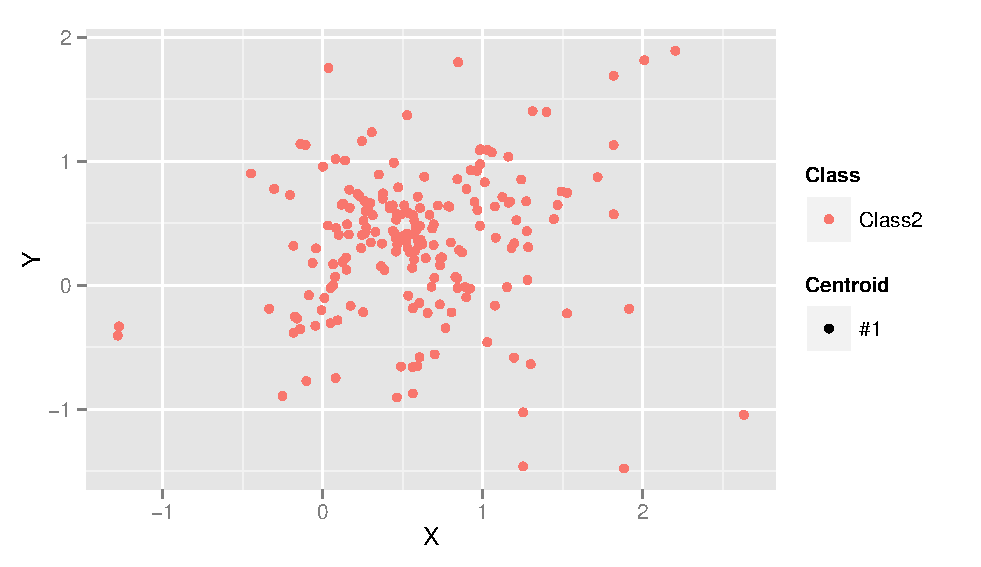
\includegraphics{figs/drift-0.pdf}} &
            \resizebox{75mm}{!}{\includegraphics{figs/{drift-0.01}.pdf}} \\
            \scriptsize{(a)} & \scriptsize{(b)\vspace{2mm}} \\
            \resizebox{75mm}{!}{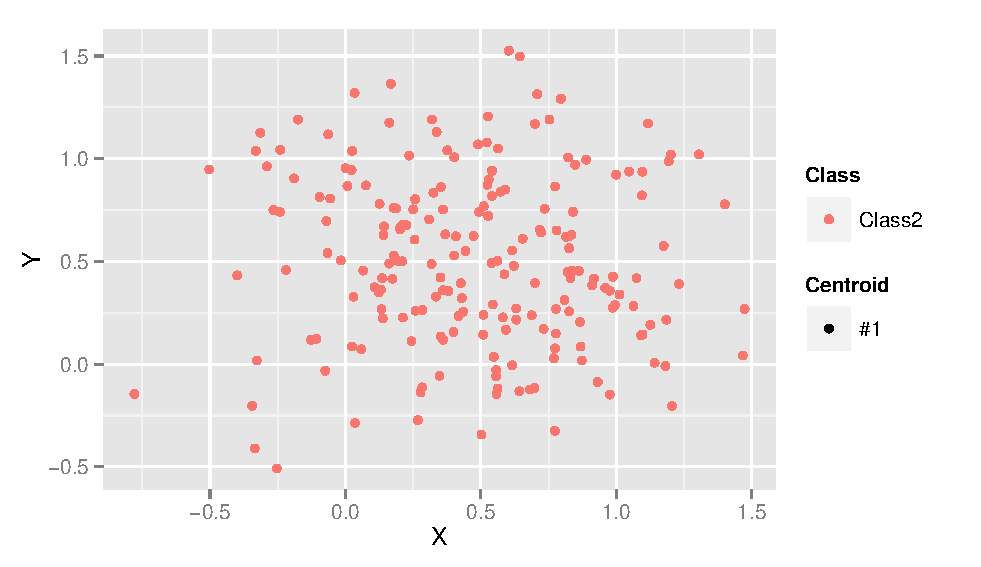
\includegraphics{figs/drift-1.pdf}} &
            \resizebox{75mm}{!}{\includegraphics{figs/{drift-0.1}.pdf}} \\
            \scriptsize{(c)} & \scriptsize{(d)}
        \end{tabular}
        \caption{RBF data generation with concept drift. Drift coefficient: (a) 0.0, (b) 0.01, (c) 0.1, and (d) 1.0}
        \label{fig:ds:rbfdrift}
    \end{center}
\end{figure}

Figure~\ref{fig:ds:rbf} illustrates a generated data set on two dimensional space with no concept drift and based on 5 centroids. Figure~\ref{fig:ds:rbf}a shows the distribution of the instances, and Figure~\ref{fig:ds:rbf}b presents the histogram of the 5 centroids from which data are generated. The differences among the centroids' weights are clearly visible here. However, it is to notice here is that the overall data set is somewhat balanced in terms of class distribution.

Next, in Figure~\ref{fig:ds:rbfdrift} we present 4 generated data sets with only one centroid, hence all instances belong to one class. Different drift coefficients have been applied to the generation process. Figure~\ref{fig:ds:rbfdrift}a, \ref{fig:ds:rbfdrift}b, \ref{fig:ds:rbfdrift}c, and \ref{fig:ds:rbfdrift}d have a drift coefficient of 0, 0.01, 0.1, and 1 respectively. As it can be seen, the instances are more compact when there is no concept drift. The introduction of a small concept drift gradually moves the concepts away. With a higher drift coefficient, instances become sparser. That is with higher drift coefficient, it would become harder for the model to learn a concept, as the required set of rules will keep changing.

We retain most of these properties of a RBF generator in creating our Variable Speed RBF Stream (VSRBF) generator. We want the data set to be balanced in terms of the binary class distribution. We also want some centroids to produce more data at higher speed, possibly, with higher drift while some centroids to produce fewer data with very little drift in a certain time frame. With these goals, we present the data generation process for variable speed RBF Stream in the next chapter.

\section{A New Approach to Generate Varying Speed Data Streams}
To generate a variable speed RBF stream, we replace the concept of centroids with pools of centroids where each pool is associated with specific properties such as weight, activation percentage, drift coefficient etc. The weight determines how much a pool would contribute to the final stream. The activation percentage is used to determine what percentage of the centroids would produce data at any given time. For slower pools activation rate would be larger, and for faster pools this would be smaller. At the start of the generation process a sufficient number of centroids is generated and assigned randomly to a user specified number of pools. The generation process of centroids remain exactly the same as the RBF generator: a randomly chosen point in the hyper-space with a randomly assigned class label. Instances generating from each centroid have this point as the mean of the normal distribution with a randomly selected standard deviation. After assigning these centroids into pools, the pools are assigned relative weights. We have used linearly increasing and quadratically increasing weights for experiments. Drift coefficients associated with all the centroids within a pool are the same and also follow a quadratic rate among the pools. As we mentioned before, slower pools i.e. pools with lower weights have lower drift coefficients than the pools with higher weights.

\begin{algorithm}[htbp]
    \caption{Varying Speed RBF Generator}
    \label{alg:vsrbf}
    \DontPrintSemicolon
    \SetKwInOut{Input}{Input} \SetKwInOut{Output}{Output} 
    
    \Input{$p$: Number of pools \\
        $b$: Batch size \\
        $m$: Number of centroids \\
    } 
    \Output{$D$: A data stream}
    
    \Begin{
        Create $p$ pools: $pools$ \\
        Generate $m$ centroids: $centroids$		  	\tcp*[f]{Sufficiently large number, $m \gg p$} \\
        Distribute $centroids$ to $pools$ randomly \\
        
        \ForEach{$p_i \in pools$} {
            Assign weights, activation percentage, drift coefficient to the $pools$ \\
            $w_i = f_1(i)$		  			\tcp*[f]{$f_1()$ is linearly/quadratically increasing} \\
            $a_i = f_2(i)$		  			\tcp*[f]{$f_2()$ is linearly/quadratically decreasing} \\
            $d_i = f_3(i)$		  			\tcp*[f]{$f_3()$ is linearly/quadratically increasing} \\
        }
        \While{$true$} {
            \ForEach{$p_i \in pools$} {
                Randomly activate $a_i$ fraction of centroids in $p_i$ \\
            }
            {\tiny {\tiny }}
            \ForEach{$p_i \in pools$} {
                $n_i = b*w_i/ w$ where $w = \sum w_i$ \\
                Generate $n_i$ instances \\
            }
            Randomly shuffle all generated instances \\
            Add instances to $D$ \\
        }
        Return $D$
    }
\end{algorithm}

To mimic concept evolution and recurrence, we associate each pool with an activation percentage that determines the percentage of centroids within the pool that are activated. If a centroid is not activated, it will not produce any instance until it gets activated again. Slower pools has higher activation percentages. With these settings, the pool with the highest weight will produce a burst of instances belonging to only a few centroids while the pool with the lowest weight will produce small number of instances from a higher number of centroids. As mentioned before, these centroids are also associated with less drift. Thus, essentially we would get slow but consistent concepts.


\begin{figure}[htbp] 
    \begin{center}
        \begin{tabular}{cc}
            \hspace{-5mm}\resizebox{90mm}{!}{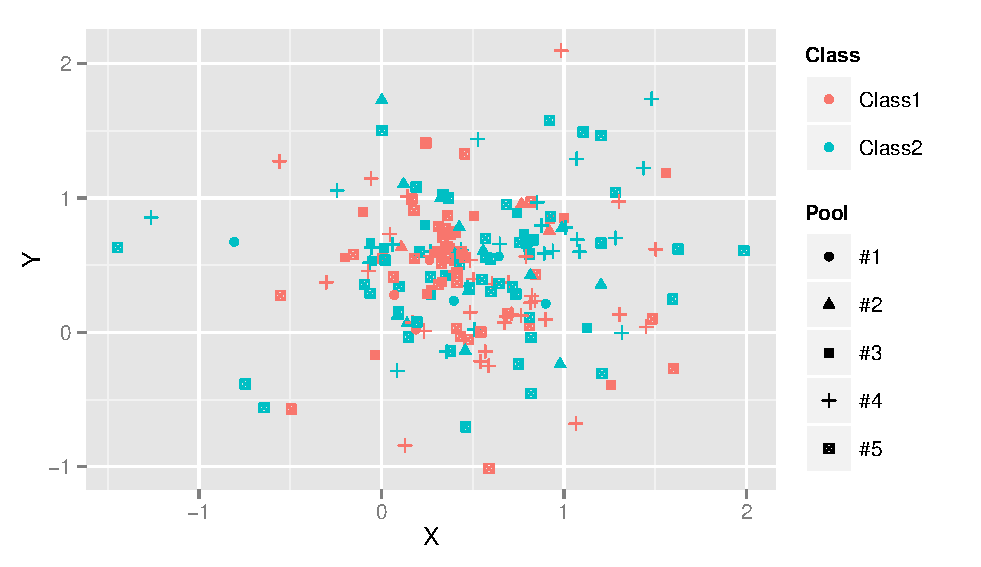
\includegraphics{figs/var5x2.pdf}} &
            \hspace{-10mm}
            \resizebox{70mm}{!}{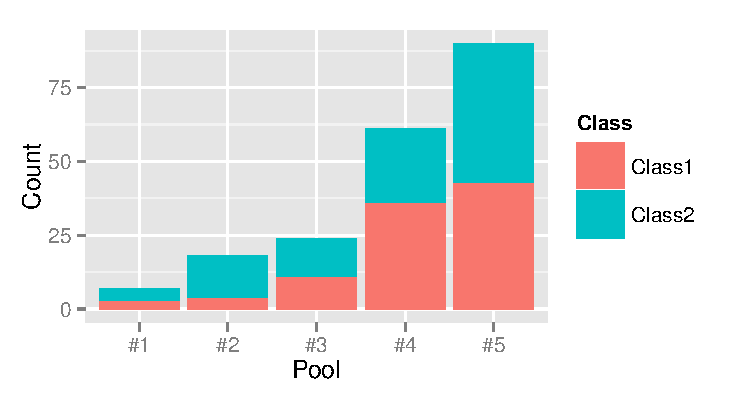
\includegraphics{figs/var5x2-hist.pdf}} \\
            \scriptsize{(a)\vspace{2mm}} &
            \scriptsize{(b)}    
        \end{tabular}
        \caption{Varying speed data generation with 5 centroids in 2D space (a) distribution (b) histogram}
        \label{fig:ds:varspd}
    \end{center}
\end{figure}

For the ease of implementation, we achieved this weight  variation and activation among the pools by generating instances in batches. Each batch starts by configuring the pools. The activation of centroids is updated randomly based on the activation percentage at each configuration. It randomly activates the required number of centroids based on the associated activation percentage of the pools. For each batch, each pool generates a certain number of instances depending on its weight. Contributions from all the pools are then shuffled randomly. The batches serve as reservoirs. Once a reservoir gets depleted, the next batch fills the reservoir. Algorithm~\ref{alg:vsrbf} presents the pseudo-code of the generation process.

\begin{figure}[htbp] 
    \begin{center}
        \begin{tabular}{c}
            \resizebox{130mm}{!}{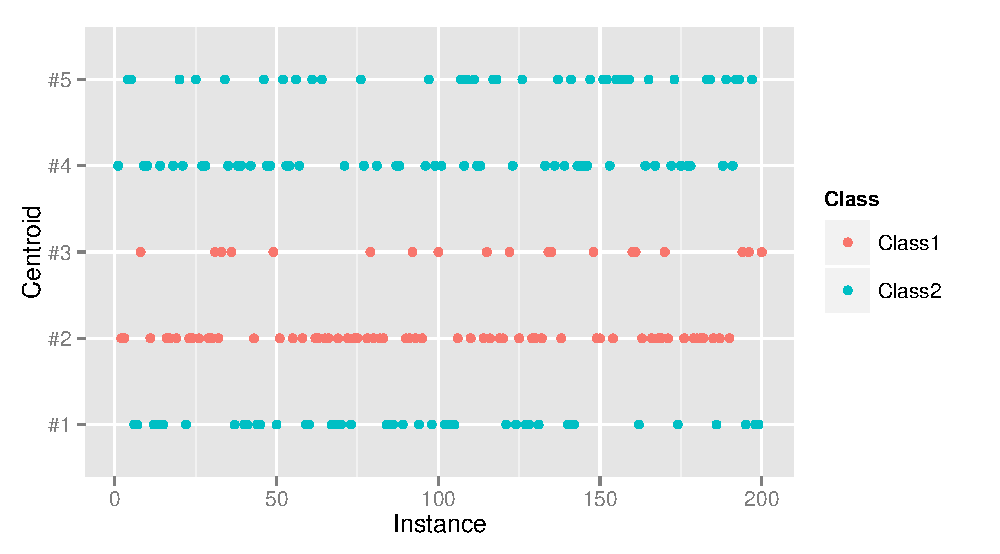
\includegraphics{figs/rbf-ivc.pdf}} \\
            \scriptsize{(a)\vspace{2mm}} \\
            \resizebox{130mm}{!}{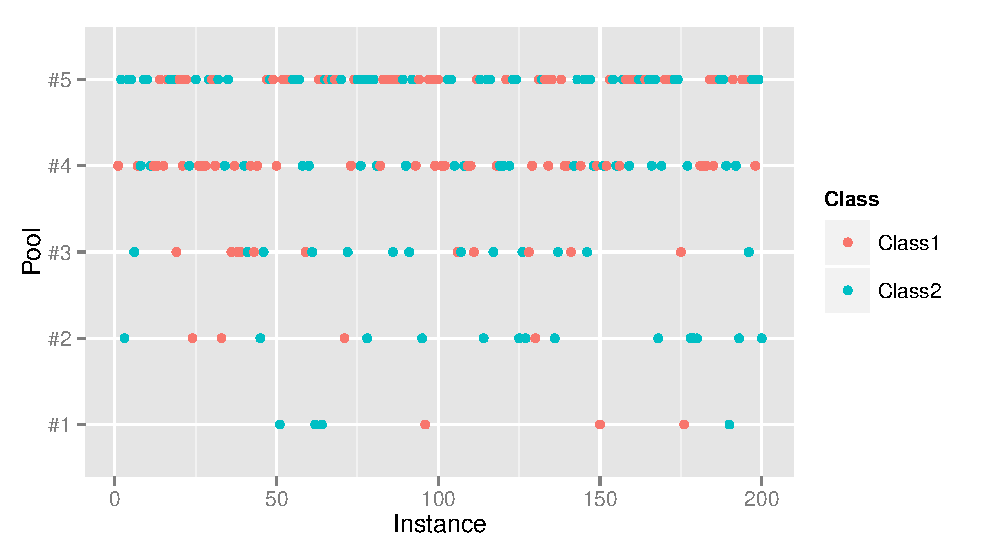
\includegraphics{figs/var-ivp.pdf}} \\
            \scriptsize{(b)}    
        \end{tabular}
        \caption{Timeline of instances (a) random RBF generator with 5 centroids (b) variable-speed RBF generator with 5 pools and 40 centroids}
        \label{fig:ds:ivcp}
    \end{center}
\end{figure}

Figure~\ref{fig:ds:varspd} presents a generated data set with 5 pools. As the histogram indicates, the $4^{th}$, and $5^{th}$ pools produce a significantly higher number of instances compared to the $1^{st}$, $2^{nd}$, or $3^{rd}$ pool. However, a close inspection at Figure~\ref{fig:ds:varspd}a would reveal that instances from these pools are more compact than the other two pools with a higher instance count. Another important property to notice here is that even though there is significant difference in the number of instances produced from each pool, the overall data set is somewhat balanced.


\begin{figure}[htbp] 
    \begin{center}
        \resizebox{130mm}{!}{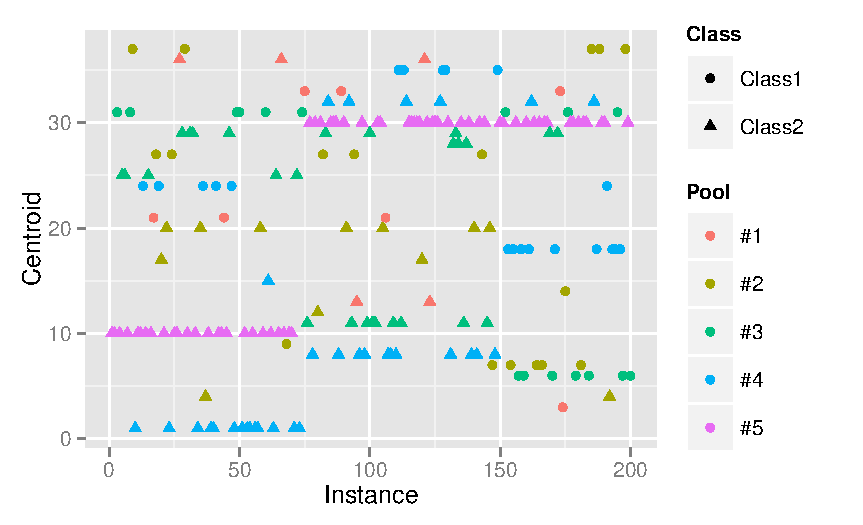
\includegraphics{figs/var-ivsc.pdf}}
        \caption{Timeline for contributing centroid in variable-speed RBF generator}
        \label{fig:ds:ivsc}
    \end{center}
\end{figure}

Lastly, it is to be noticed here that even though slower pools produce less instances than the faster ones, they are expected to be distributed in the entire time frame. Figure~\ref{fig:ds:ivcp} confirms that expectation. In Figure~\ref{fig:ds:ivcp}a, we show the timeline for a generated data set with the RBF generator with 5 centroids. It shows that each centroid generates throughout the generation process. Similarly, in the data set generated by the variable speed RBF generator, the data are generated by every pool, throughout the generation process (Figure~\ref{fig:ds:ivcp}b). The slowest pool (pool1) produces less data, but it does not do so in a fraction of the time frame. 

Moreover, in Figure~\ref{fig:ds:ivsc}, it shows a timeline for the all contributing centroids. Values are set such that at each timestamp there are about 75 instances, thus there are 3 different timestamps in the plot. Looking into the figure, it can be easily seen that for the 5th pool, at the beginning only Centroid10 is producing data. For the rest of the two timestamps Centroid30 is producing data. Similarly, for the 4th pool, at the beginning two centroids produces data: Centroid01 produces Class2 data and Centroid24 produces data from Class1. They also stop producing for the next two timestamps. For Pool3, Centroid29 is active all the time, while other change their activation. For the other two pools most of the centroids are mostly active for all three timestamps.





To summarize, in this chapter we demonstrated that the variable speed RBF generator is able to produce a stream that mimics the behaviors or properties of the streams introduced in Section~\ref{sec:intro:motiv}. In the next chapter, we use such data set to evaluate our approaches.

\chapter{New Hoeffding Tree Based Ensemble Approach}
\label{chp:algo}
In the previous chapters, we have presented the motivations, fundamental concepts, solution overview of this thesis. We have also presented the dataset generation process. Now, in this chapter, we present our algorithms, Size Restricted Hoeffding Tree (SRHT) and Carry-over bagging. Size restricted Hoeffding tree is extended from original Hoeffding tree algorithm and incorporates ADWIN method. Carry-over bagging is developed over the concepts of Oza online bagging approach.

Before, discussing the algorithms, we define our problem mathematically and re-state the solution overview. 

\section{Problem Statement}
Various modern application areas produces huge amount of data or so-called data streams. Most state-of-the-art stream mining methods generalize all application areas by similar streams. Assumptions are made that streams are generated from constant generators with concept following a certain distribution. The concepts itself may drift or evolve, but overall nature of the generators remain the same.

Close examination of certain application domain such as social media, WWW, telecommunication, etc. suggests that streams are decomposable in smaller sub-streams, possibly in a mutually exclusive manner. These sub-streams differ can differ significantly in the way they generate or contribute to the overall stream. Some of these sub-streams are very short-lived but produces extremely high number of instances, whereas some are always present and consistently produces data but with relatively very slow speed.

Generalizing such streams with a generator that does not reproduce such scenarios might not produce the expected result. Performance measure such as overall accuracy, may fail to indicate limitations of learners in such environment.

In Chapter~\ref{chp:dataset}, we demonstrated how to synthesize a dataset with speed varying properties. With these types of datasets, current state-of-the-art methods faces trouble in learning the slower streams. As it takes longer time to accumulate sufficient information for the concepts with slower speed, only those classifier with larger capacity and longer lifetime would contain decision rules for slower concepts. Then again, we have usual challenges with concept drift, size of the classifier, over-fitting, etc.

With these motivations, we define our problem statement as follows:

\begin{quotation}
    \textbf{Online classification of data streams, that are decomposable into speed-varied sub-streams, with decision tree based approaches.}
\end{quotation}

\noindent Formally, given a stream $S$ of very high volume, possibly infinite, having a set of $m$ nominal or continuous attributes $X$, where each instance has a class label from a set $Y = \{y_1, y_2, \dots, y_k\}$, we want to build a classifier that is able to predict the classes of incoming instances at any given time. Note that, this definition is very general, and can be used for any of the present learner. The uniqueness lies the in nature of stream $S$. We want to improve the performance when $S$ is a composite stream, composed of a set of sub-streams with huge contribution differences.


\section{Solution Overview}
Like all other stream learning algorithms, there are 3 most important aspects that needs to be addressed in our potential learning algorithm. These are (i) the model has to be updated to be able to classify most recent data, (ii) the model has to detect concept drifts and to be updated accordingly, and (iii) model must no grow to be very complex causing over-fitting. Along with these requirements for our problem, additionally, (iv) it needs to perform equally good for different concepts within the classes. As the arguments were made before, fulfilling this new requirement is challenging because of first two requirements. To keep the model up-to-date with the data and the concept, effect of older concepts and data need to be removed from the model. In doing so, very easily we end up losing information of the slower sub-streams. As the faster sub-streams produces high volume of data, the model is always dominated by those concepts. Slower sub-streams initially gets classified wrongly, then over time when the model gathers enough information about these slower streams or concepts, new rules emerges for those concepts. However, these rules become `old' very soon with the incoming volume of faster concepts. As a result, in most of the current state-of-the-art stream mining methods, these rules will get pruned after a while to keep the model update to data and concept.

To achieve the fourth goal, we modified few of the existing methods and used them in a combination. From the methods discussed in Chapter~\ref{chp:background}, we learned a few methods of learning a decision a tree and keep it updated with the newer concepts. Let's first analyze what are the possible approaches that can be taken to keep a model updated to the newer concepts and data, and how to get rid of the older concepts.

\subsection{Incrementally Growing Tree}
Using methods such as Hoeffding Tree (Section~\ref{sec:bg:vfdt}) would result in a incremental tree with time. Hoeffding tree keeps itself updated by spanning to the entire feature space and changing the weights values within the leaves. Theoretically, with sufficiently large learning time and diverse data instances, Hoeffding will span the entire feature space with all possible combinations.

\begin{figure}[htbp]
    \begin{center}
        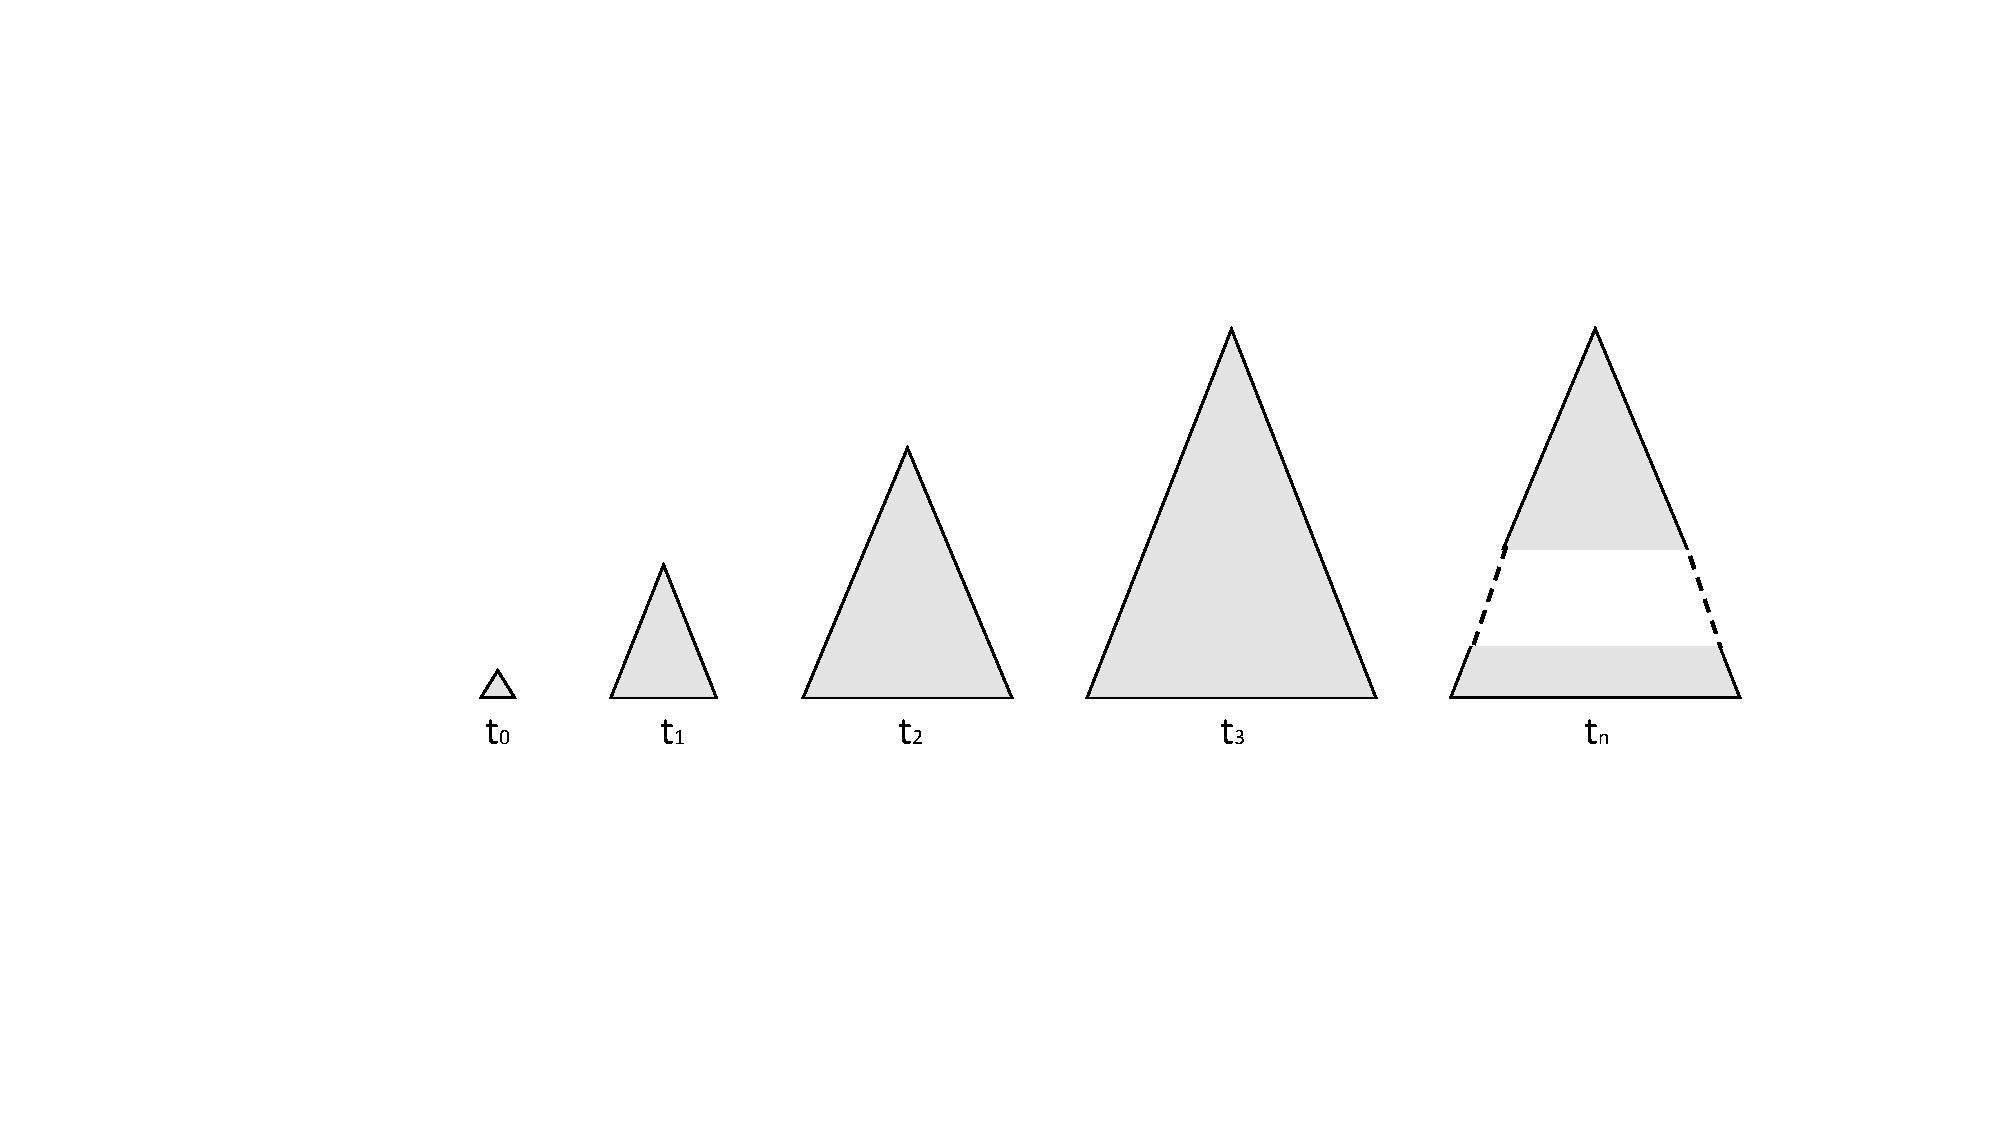
\includegraphics[width=14.0cm]{figs/infgrow.pdf}
        \caption{Incrementally expanding tree}
        \label{fig:algo:infgrow}
    \end{center}
\end{figure}

Figure~\ref{fig:algo:infgrow} shows how the size of the tree may change over over time. At $t_0$, it starts with a single node, and keeps expanding as the time passes. A hypothetical corresponding decision boundaries in 2D space are shown in~\ref{fig:algo:infgrowdb}. As the figure shows, with the the model become complex and prone to the slightest changes in data.

\begin{figure}[htbp]
    \begin{center}
        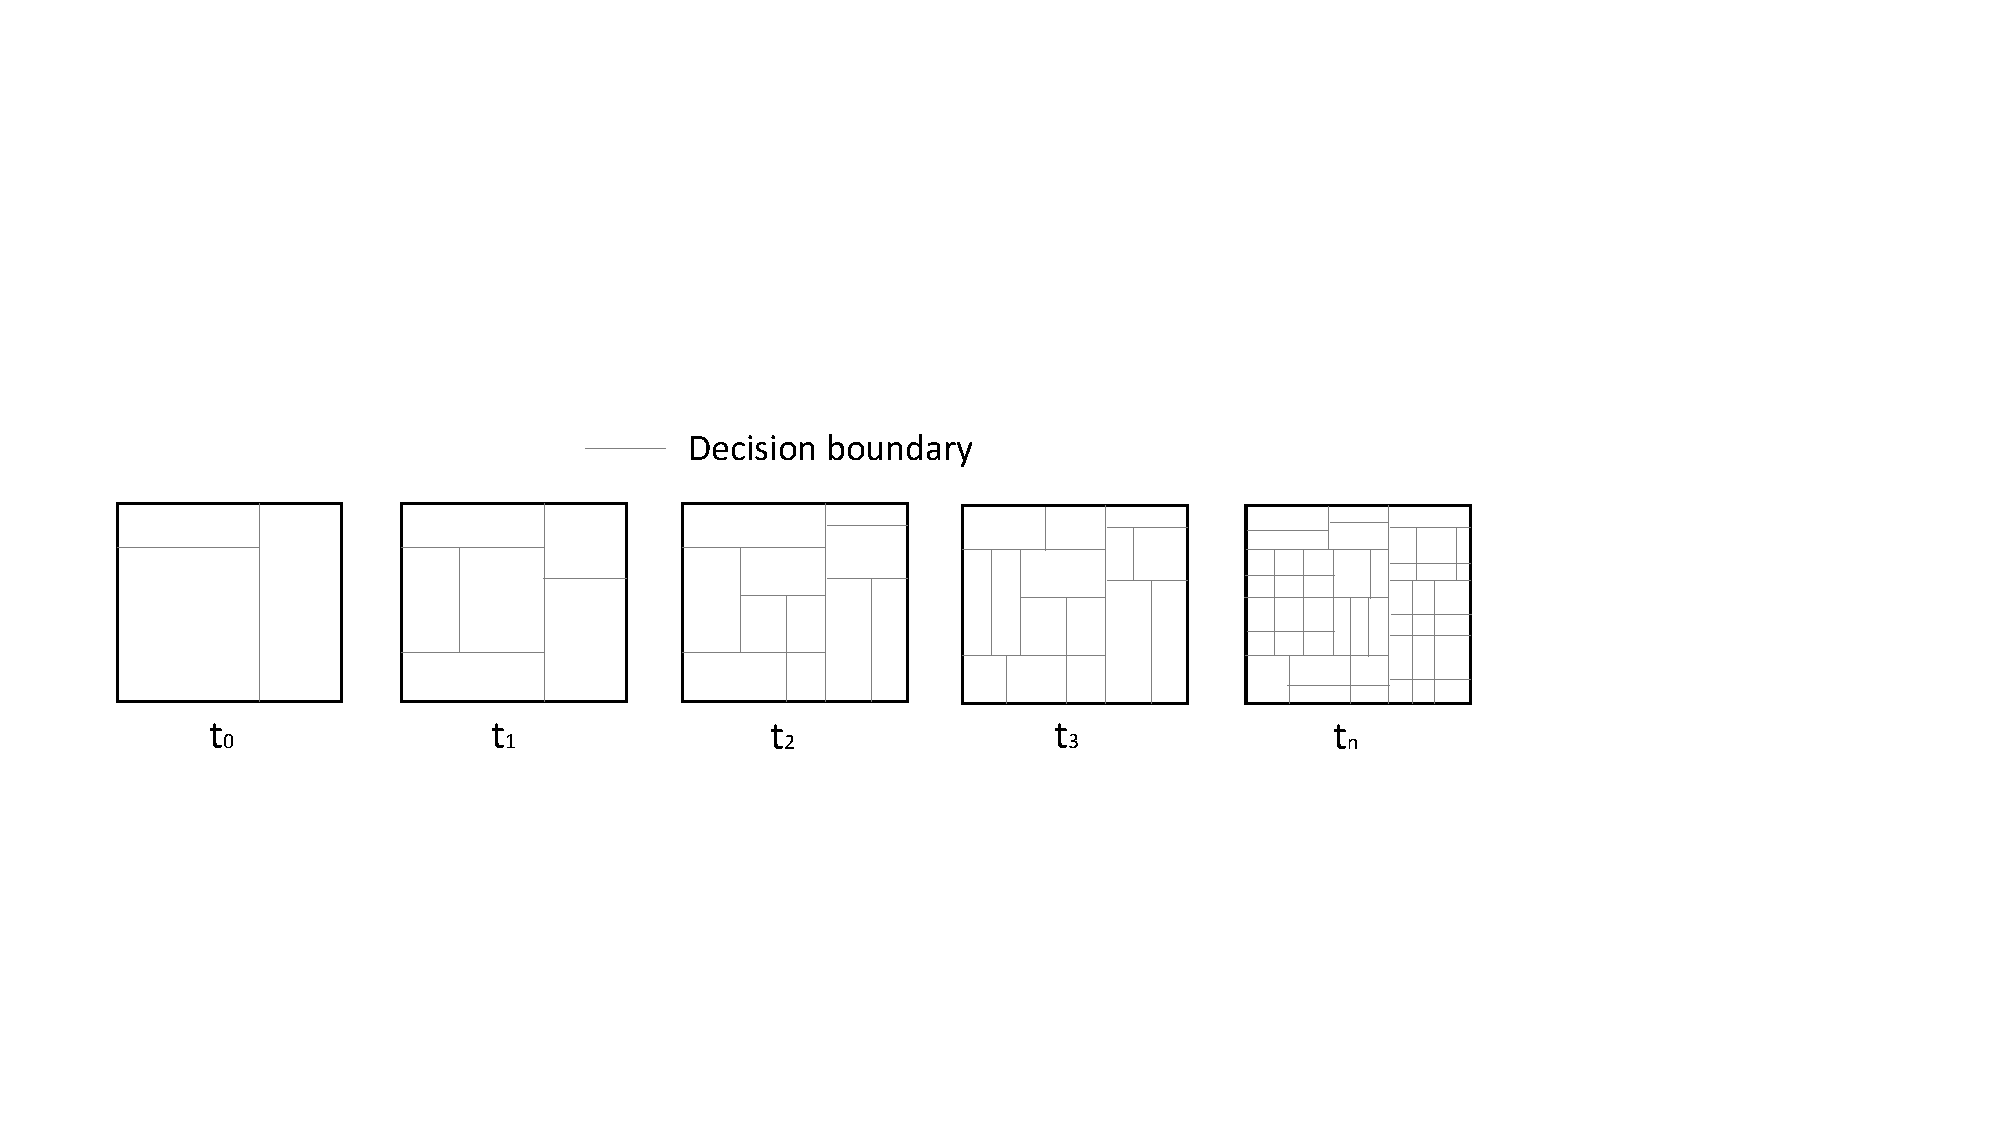
\includegraphics[width=14.0cm]{figs/infgrowdb.pdf}
        \caption{Decision boundaries for infinitely expanding tree}
        \label{fig:algo:infgrowdb}
    \end{center}
\end{figure}


\subsection{Reseting Tree}
The scheme of incrementally growing Hoeffding tree is simple and easy to implement. However, one of the major shortcomings of this approach is that, it leads to over-fitting. As there are abundance of training instances, after a period, the model starts following the instances rather than trying to realize the underlying relations. One way to stop that from happening is to reset the tree once in a while (Figure~\ref{fig:algo:reset}). This reset could be triggered by some time dependent event, or it could also be dependent on some property of the tree. For example, depth of the tree, size or number of nodes in the tree, number of decision nodes in the tree, etc. can be used as a trigger with a maximum threshold bound.

\begin{figure}[htbp]
    \begin{center}
        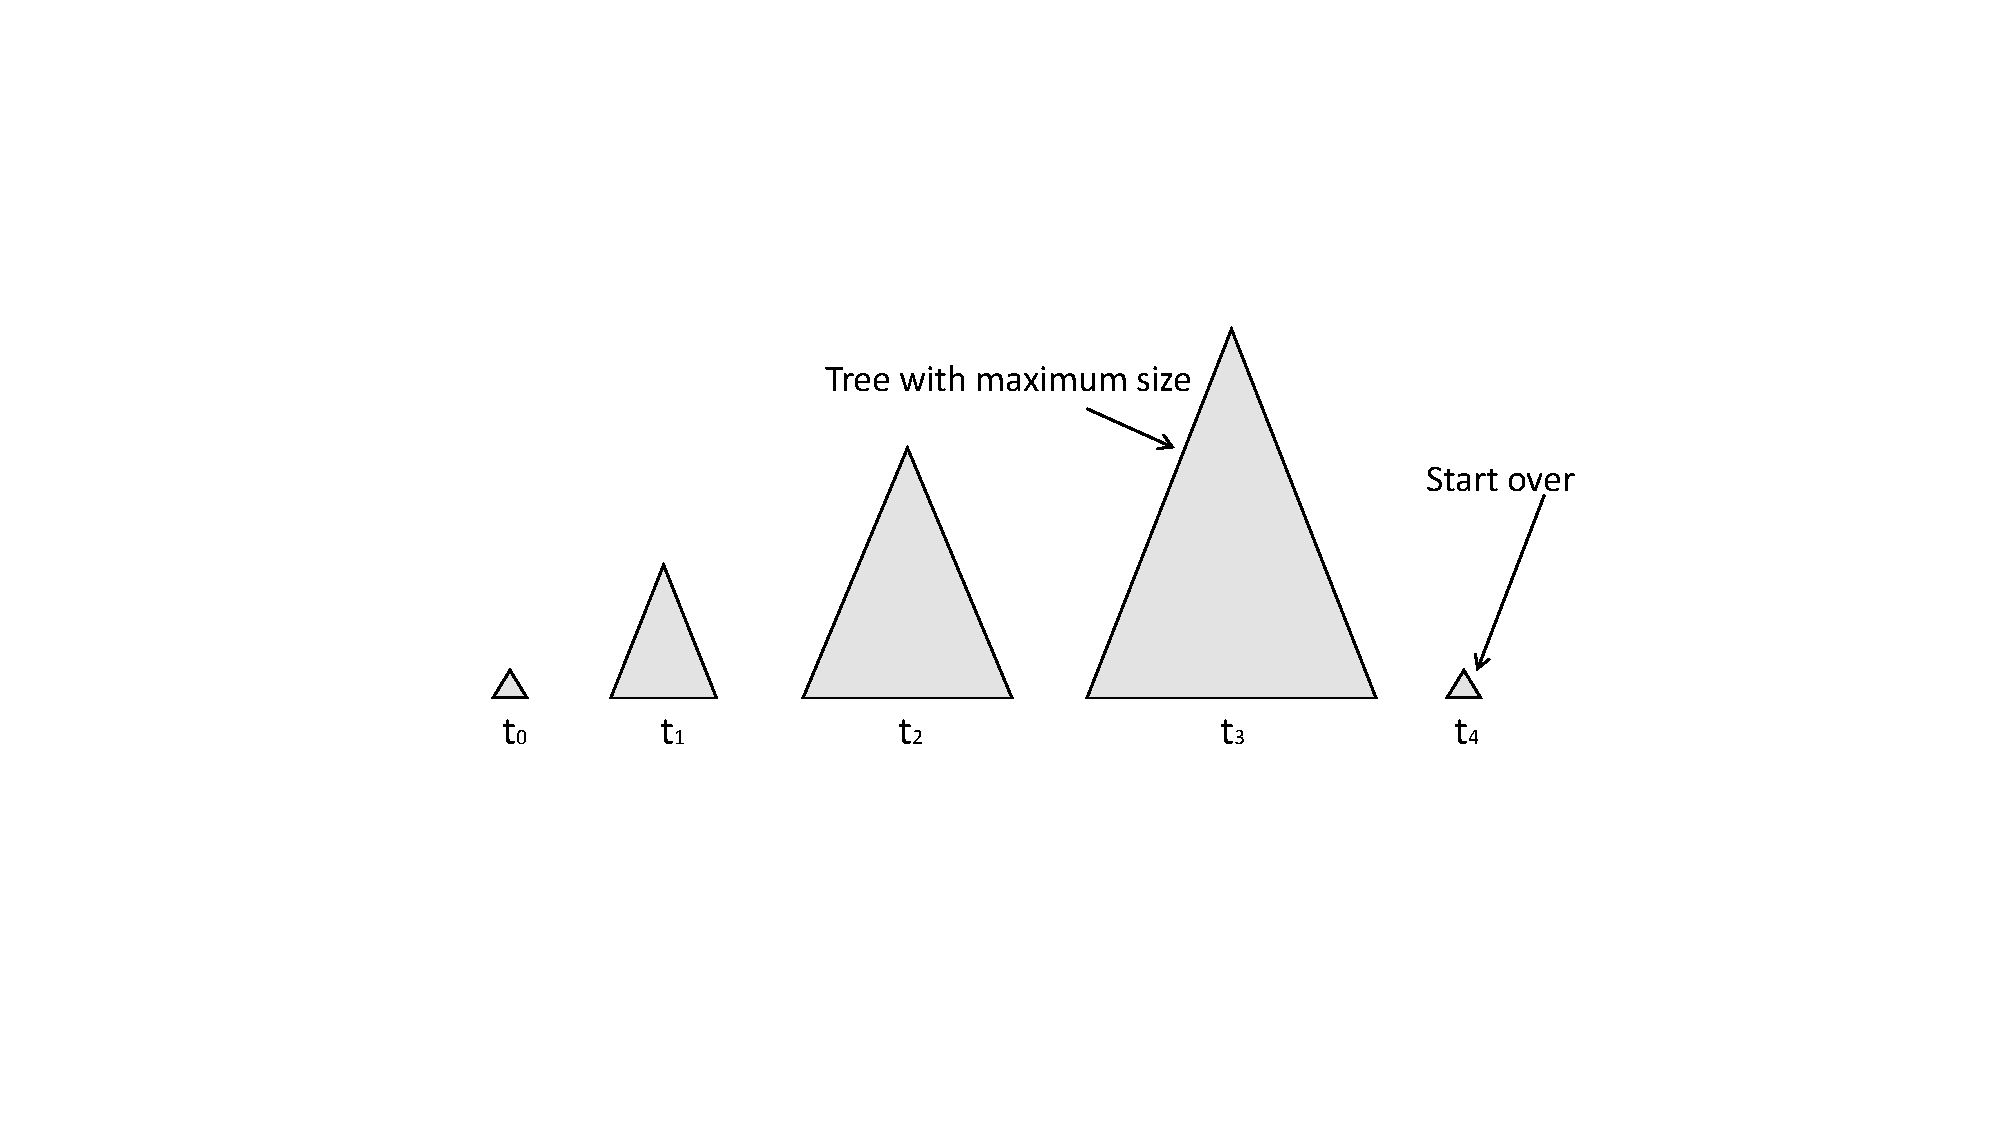
\includegraphics[width=12.0cm]{figs/reset.pdf}
        \caption{Reseting entire tree upon reaching threshold size}
        \label{fig:algo:reset}
    \end{center}
\end{figure}


Essentially, by reseting the entire tree, the model starts learning from scratch again. Every decision rule learned from observed data are lost (Figure~\ref{fig:algo:resetdb}). However, it does also get rid of all the biases that were present in the observed data for the incoming data. In Adaptive Size Hoeffding Tree (ASHT) bagging, this reset idea has been used in association with an ensemble of different sized ASHTs (Section~\ref{sec:bg:asht}). As the size threshold is different for the trees in the ensemble, the probability of all being reset at once is very less. Thus by using the idea of reseting trees in an ensemble allows the model to retain important information upon a reset of a tree in the ensemble. However, it is important to understand that reset of smaller trees in ensemble have much lesser effect than the reset of larger trees. Smaller trees in the ensemble targets recent data, and there are abundance of that. On the other hand, larger tree contains information learned over a longer period, thus also containing small but important concepts. This is exactly what we want to retain.

\begin{figure}[htbp]
    \begin{center}
        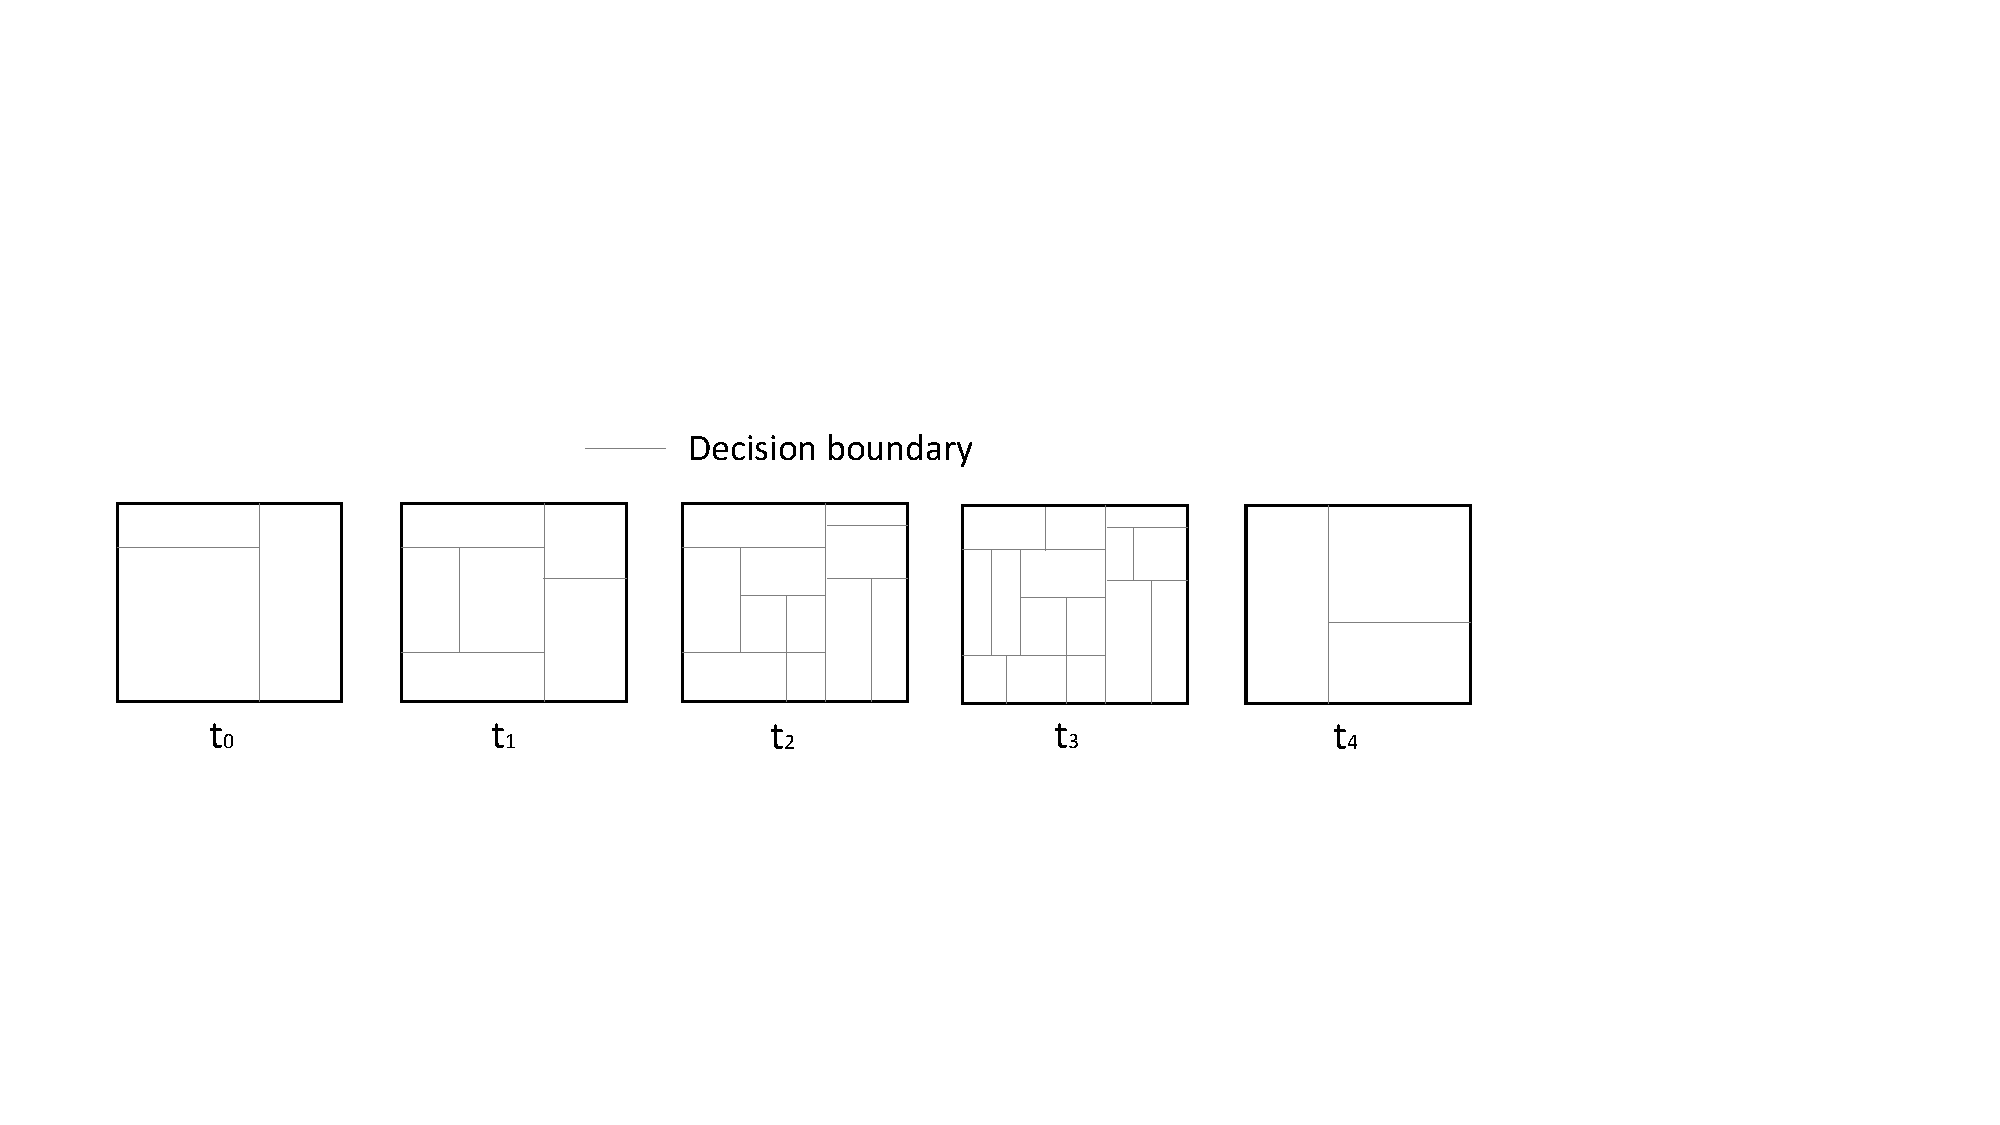
\includegraphics[width=14.0cm]{figs/resetdb.pdf}
        \caption{Decision boundaries after tree reset}
        \label{fig:algo:resetdb}
    \end{center}
\end{figure}

\subsection{Pruning by Deleting Older Nodes}
An alternate choice to reseting entire tree is to delete the older decision nodes, i.e. root or top levels. As in the Hoeffding tree, attribute choice for each level depends on newer data from the previous level, the top level decision nodes are chosen based on oldest data segments. Thus, removing the root and all its children except for the one chosen as the next root would remove the effect of oldest data. Moreover, it allows the tree to grow again as the threshold (number of decision nodes) is effectively decreased by at least 1.

\begin{figure}[htbp]
    \begin{center}
        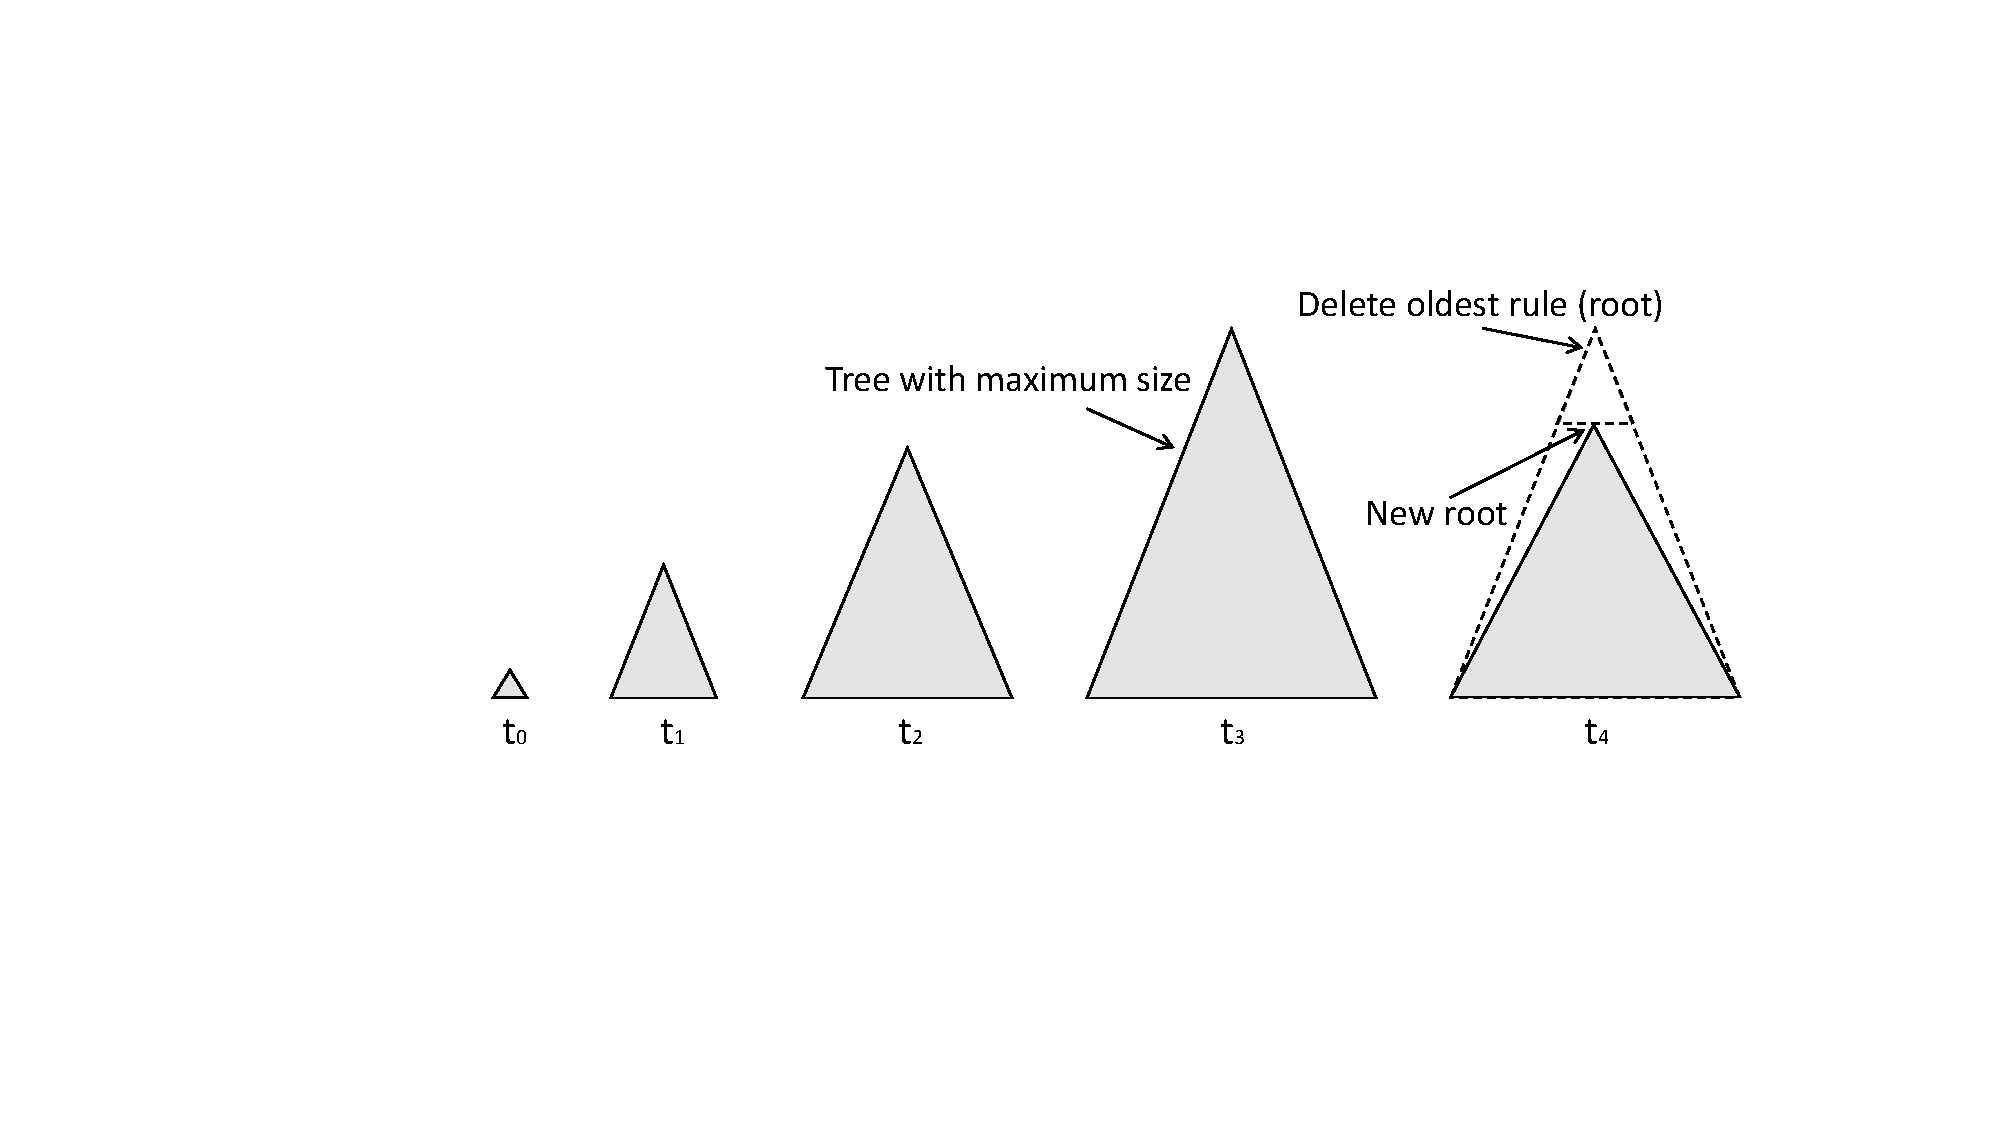
\includegraphics[width=14.0cm]{figs/deleteroot.pdf}
        \caption{Deleting the oldest branch (root) and selecting new root from its children}
        \label{fig:algo:delroot}
    \end{center}
\end{figure}

Figure~\ref{fig:algo:delrootdb} show the changes in the decision boundary upon deleting the root. As it shows, only the earliest boundaries are deleted in this process. If the model has already become too complex, then this does not improve the situation much. But for less complex models, this should for the tree to learn information within the newly merged regions. Moreover, because the order in which the checks are performed changes, the existing decision rules might change (decision class).

\begin{figure}[htbp]
    \begin{center}
        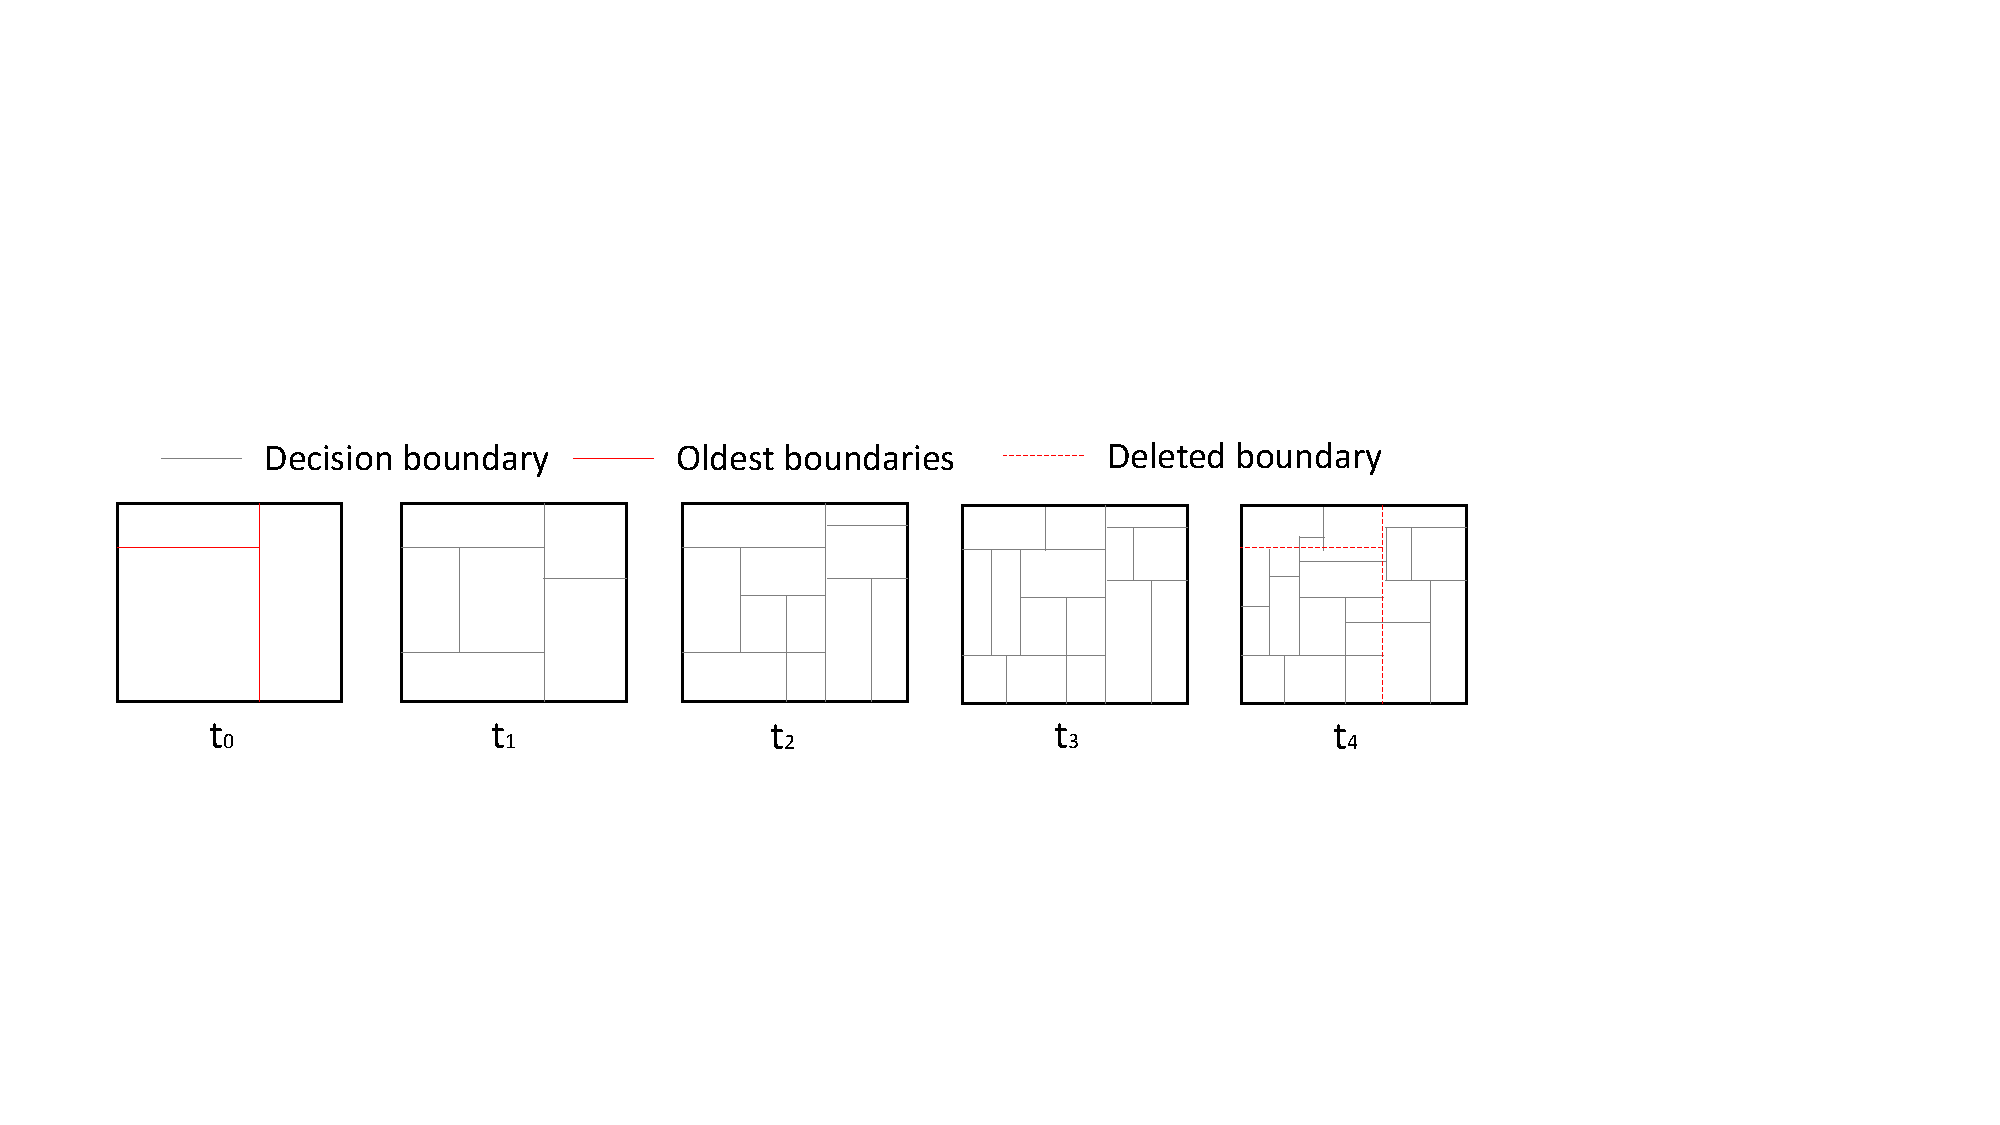
\includegraphics[width=14.0cm]{figs/deleterootdb.pdf}
        \caption{Decision boundaries after deleting root}
        \label{fig:algo:delrootdb}
    \end{center}
\end{figure}


\subsection{Pruning by Maintaining Alternate Trees}
In a different approach than deleting root or entire tree, maintaining alternate sub-tree wherever necessary can effectively maintain the model's relevance to the recent data. Adaptive Hoeffding Tree uses such approach by maintaining ADWIN (Section~\ref{sec:bg:changedetection}) to check error margin at each decision node. In case of a increase in error margin at any node, an alternate branch is initiated and learned. If in future, there is enough evidence that alternate branch performs better than the current one, then current sub-tree is replaced by the alternate sub-tree. Otherwise, the alternate sub-tree is deleted. Every time error margin exceeds main tree and the alternate tree, a new alternate branch is created. Thus, one decision node might have multiple alternate sub-tree. Note that, an alternate branch might get started at the root itself, and if it performs better, would change the entire tree with something new.

\begin{figure}[htbp]
    \begin{center}
        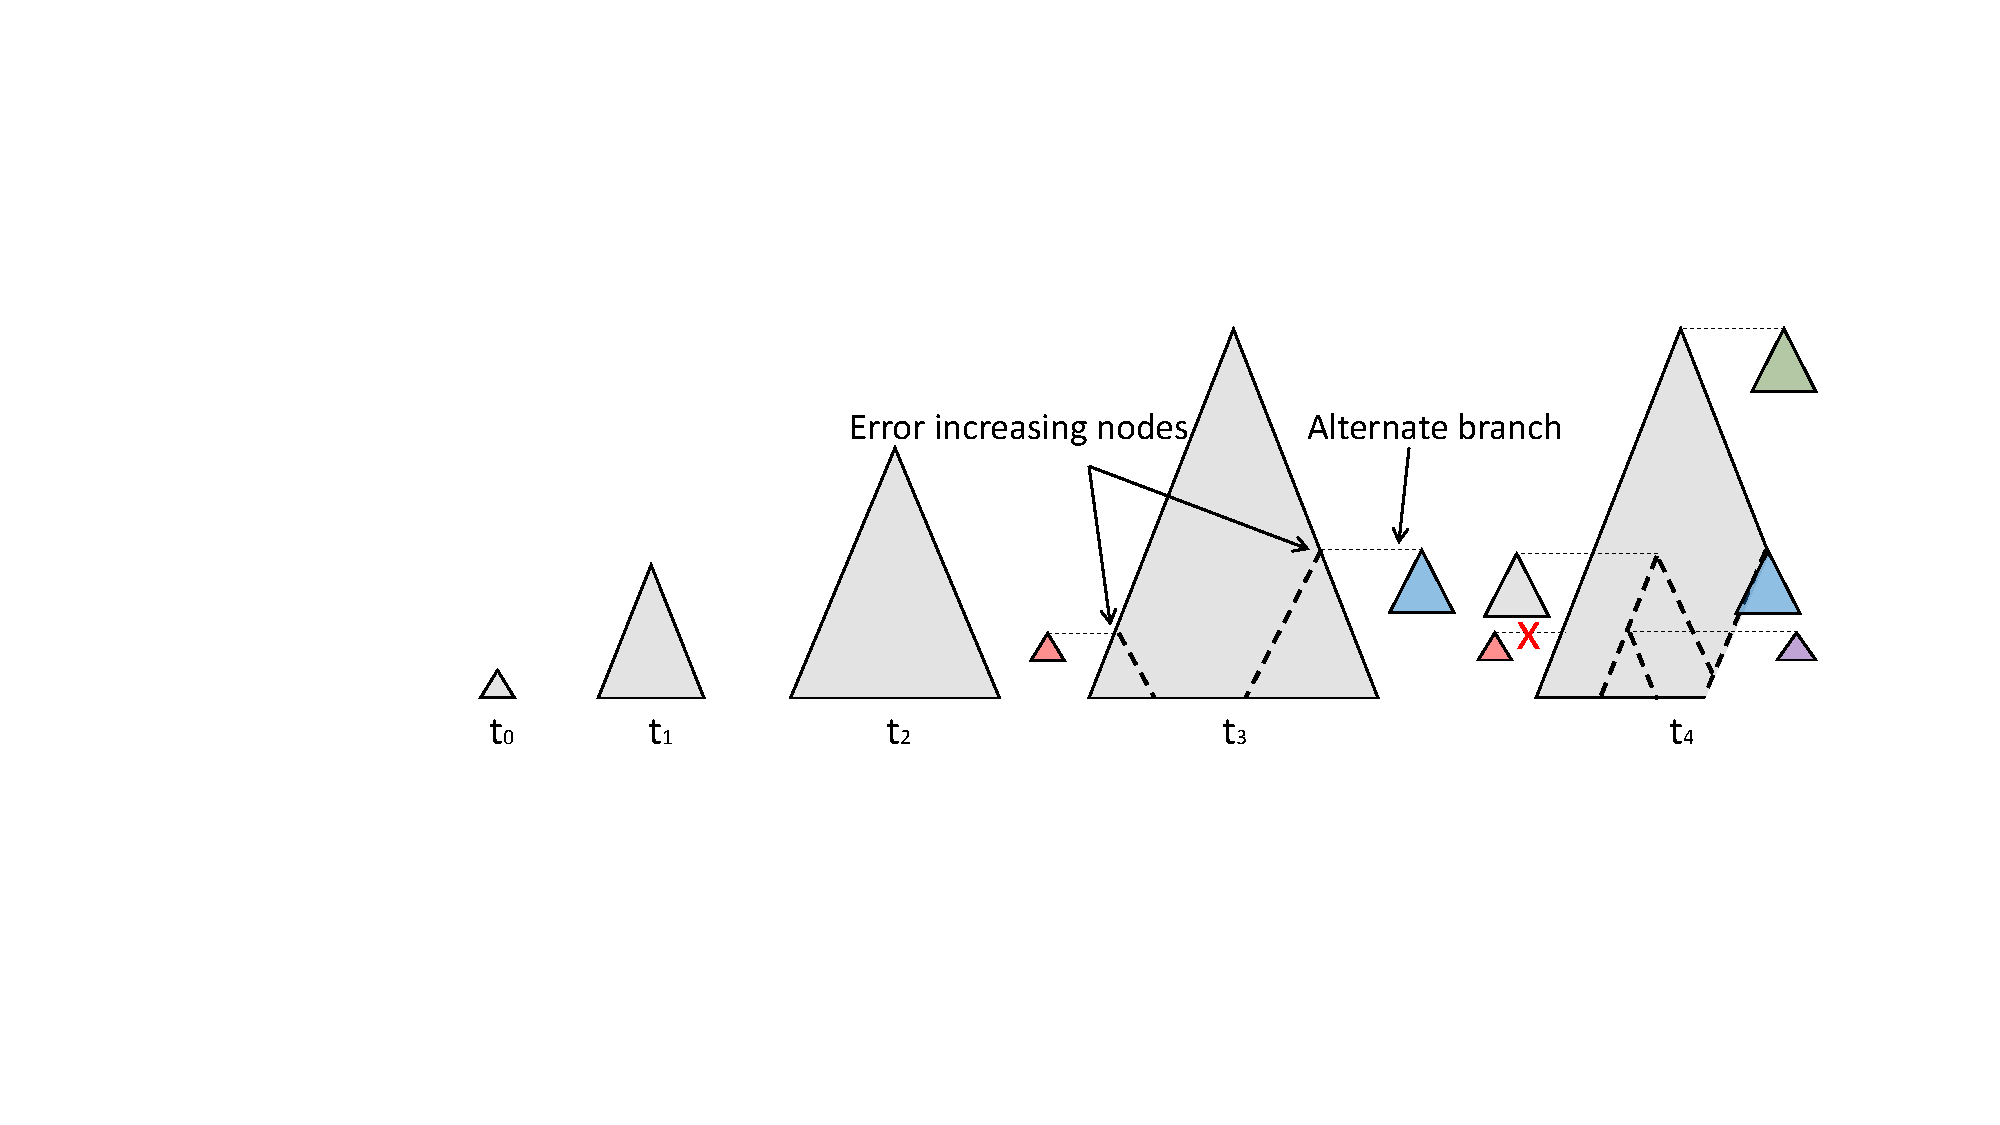
\includegraphics[width=14.0cm]{figs/prune.pdf}
        \caption{Maintaining alternate branches for pruning}
        \label{fig:algo:prune}
    \end{center}
\end{figure}

Pruning using alternate trees can effect detect changes in the concepts. As it employs ADWIN, nodes are not immediately replaced if they start performing worse than before. Rather, it waits to confirm that an actual change in the data concepts has occurred. Otherwise, it deletes the alternate tree. This way, the model is saved from being prone to outliers and very small blocks of data from other concepts. In Figure~\ref{fig:algo:prunedb}, we illustrated how the decision could change in terms of the trees shown in Figure~\ref{fig:algo:prune}. Generally, it is expected that a block of decision boundaries will be replaced by another block. It does not necessarily be a simpler one. Alternate trees, theoretically, can be larger than the block it would replace in the original tree.

\begin{figure}[htbp]
    \begin{center}
        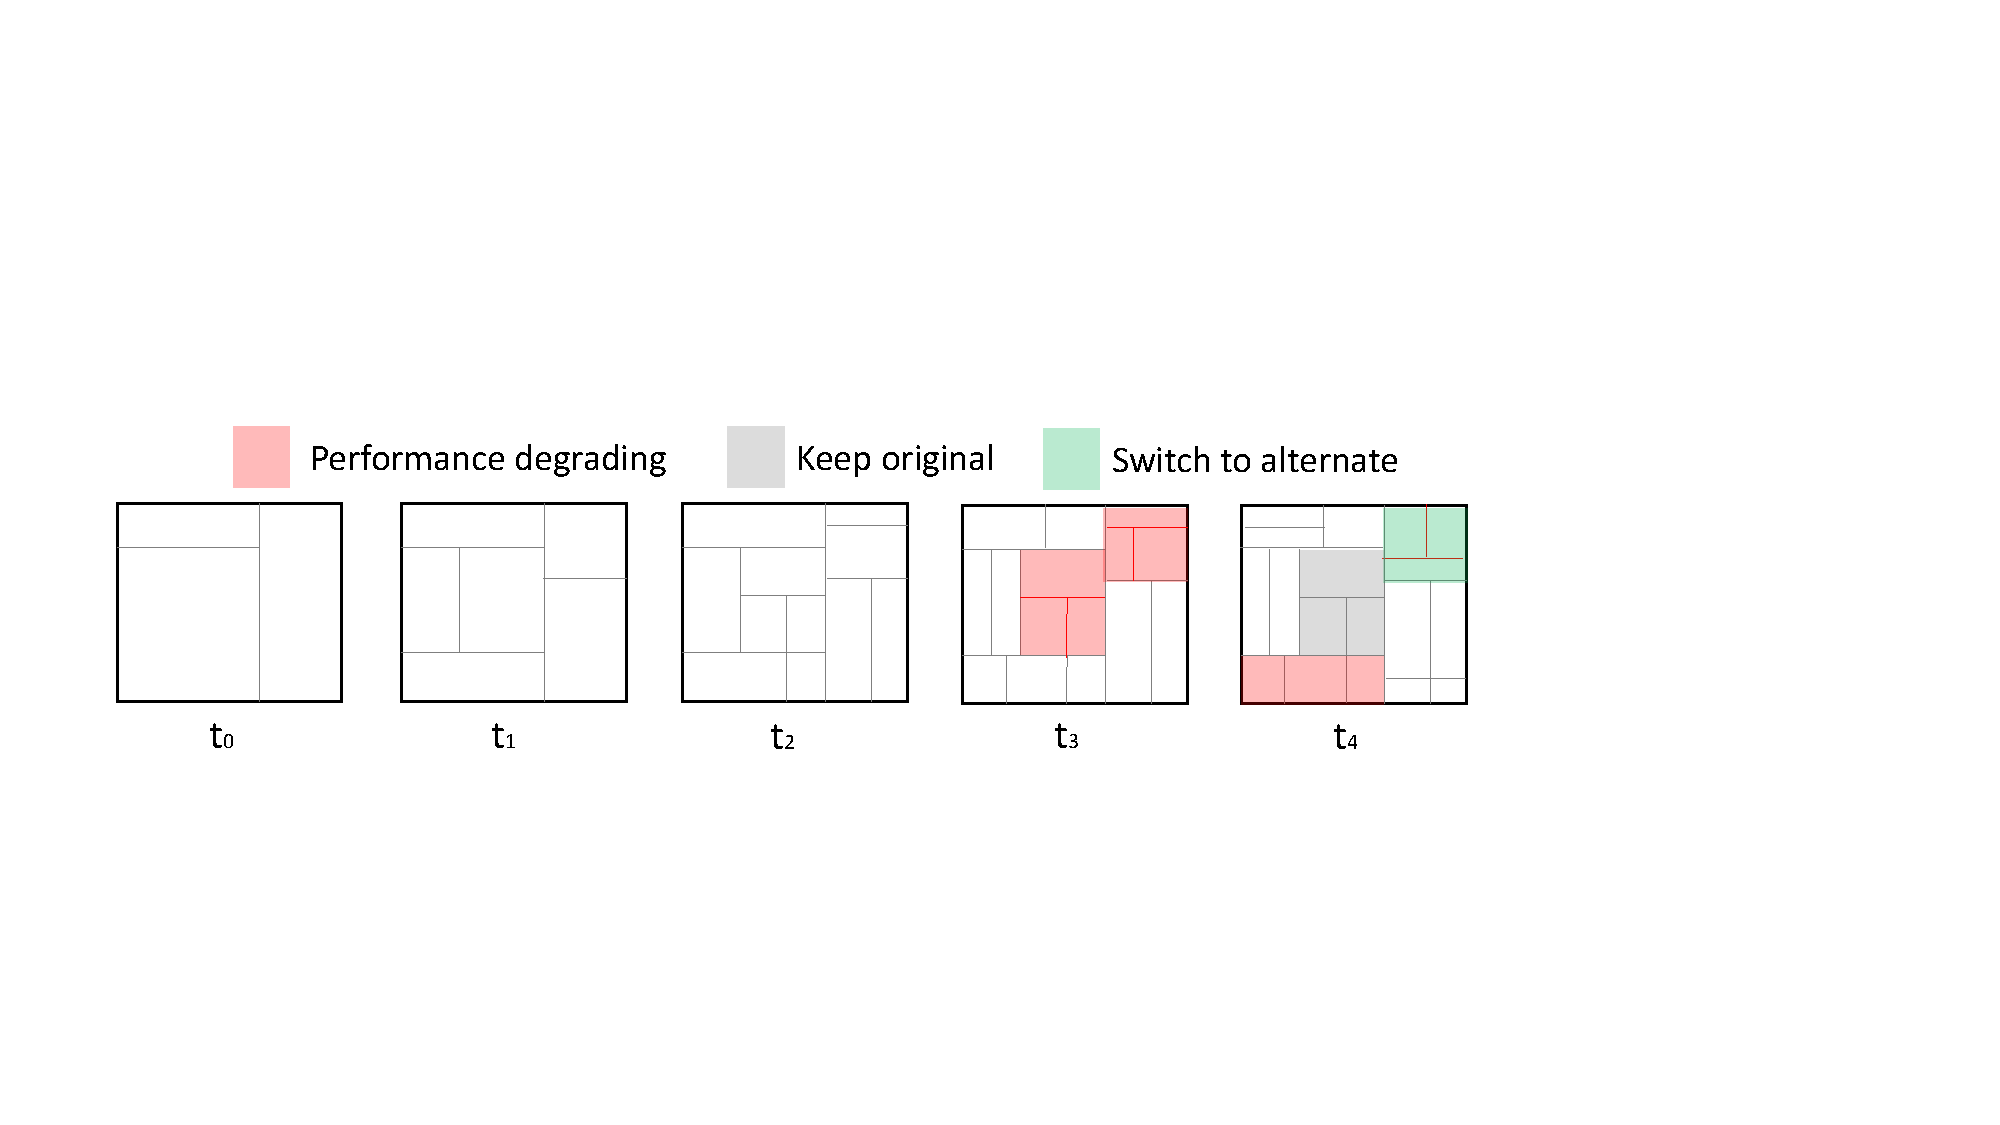
\includegraphics[width=14.0cm]{figs/prunedb.pdf}
        \caption{Decision boundaries after pruning using alternate branching}
        \label{fig:algo:prunedb}
    \end{center}
\end{figure}

\subsection{Combining the Ideas}
To approach our problem, we combine these ideas in a effective manner. Our solution is entirely motivated by assumptions made in Hoeffding tree approaches, that is to effectively decide on a splitting attribute in data streams with certain degree of accuracy, a small portion of the data might be sufficient; and the bound of accuracy can be estimated using Hoeffding bound. Based on this fundamental assumption, we combined the idea of restricting and reseting Hoeffding tree based on a threshold size in terms of number of decision nodes and the concept of maintaining alternate branches for nodes where performance are degrading using ADWIN method. Restricting the size of the tree can be used to control the amount of data the tree would be build upon. Applying ADWIN within the size restricted tree would ensure that the tree model is updated to the drifted concepts. 

As discussed earlier that immediate reset of tree is not desirable where retaining of slower concepts is a concern. Thus, we developed a bagging scheme based on ASHT bagging to delay the reset of the trees upon limit is reached. With this scheme we stop the tree growth immediately as the size limitation is reached. We start building a new tree with same size restriction. For the successive learning, both trees are learned with the exception that the old tree cannot grow. It may, however, switch to alternate branches. In cases, this might reduce the tree size and allow it to grow again. Switching to a alternate tree that would increase the tree size is not allowed. For the bagging, we maintain two sets of learners. One is same as the one from ASHT bagging. A fixed number of trees each with double the size of the previous one, first one being of size 2, typically. Other is initially empty with a fixed capacity. Once a tree in the fist set reaches its limit it is moved to second set. The second set works as a fixed sized queue, as the newer are moved from the first set, older trees gets deleted. As the smaller trees reaches the size limit very fast, a threshold is set on the size of the trees that can be moved to the second set. The trees reaching their limit below this threshold are being reset immediately. In other other words, we ``carry-over'' the larger the trees for a certain period of time even after reaching the max size. For the voting for a new instance, all classifier in both the sets contributes.

With this ``carrying-over'' concept, we essentially increase the weights of the decision rules in the larger trees. Which directly influences the problem we are addressing. The larger trees contain decision rules for slower streams. By delaying the deletion of such trees, we create a buffer time for the new classifier to learn something from the newer data, while the older one keeps voting. The voting process remain more balanced between newer and older concepts during the transition period. Because in the transition time the new classifier, having larger size limit, acts as a smaller classifier just because it has not seen enough data yet. This basically increases the voting bias towards newer concepts. With our bagging carry-over bagging, this becomes more balanced, as the larger trees would still keep voting for concepts present in older data. Algorithms devised based on the discussions above are explained in following sections.

\section{Size Restricted Hoeffding Tree (SRHT)}

\begin{algorithm}[htbp]
    \caption{SRHT: Size Restricted Hoeffding Tree}
    \label{alg:srht}
    \DontPrintSemicolon
    \SetKwInOut{Input}{Input} \SetKwInOut{Output}{Output} 
    
    \Input{$S$: Stream of examples \\
        $X$: Set of nominal attributes \\
        $Y$: Set of class labels $Y = \{y_1, y_2, \dots, y_k\}$ \\
        $G(.)$: Split evaluation function \\
        $N_{min}$: Minimum number of examples \\
        $\delta$: is one minus the desired probability \\
        $d$: Alternate tree switching bound \\
        $n_d$: Number of maximum decision nodes \\
        $\tau$: Constant to resolve ties
    } 
    \Output{$HT$: is a decision tree}
    
    \Begin{
        Let $HT \leftarrow$ Empty Leaf (Root) \\
        \ForEach{$example(x, y_k) \in S$} {
            Traverse the tree $HT$ from root till a leaf $l$ \\
            
            \eIf (\tcp*[f]{Missing class label}) {$y_k == ?$ } {
                Classify with majority class in the leaf $l$
            } {
                Update sufficient statistics \\
                \If{$ Number\;of\;examples\;in\;l > N_{min}$ }{
                    Compute $G_l(X_i)$ for all attributes \\
                    Let $X_a$ be the attribute with highest $G_l$ \\
                    Let $X_b$ be the attribute with second highest $G_l$ \\
                    Start maintaining ADWIN \\
                    
                    \uIf{error increased from previous step} {
                        Start maintaining alternate tree \\
                    }
                    \uElseIf{oldError - alternateError > $d$} {
                        \uIf{ADWIN window sufficiently big}{
                            Switch to alternate tree \\
                        }
                        \uElseIf{alternateError - oldError > $d$} {
                            Delete alternate tree \\
                        }
                    }
                    
                    Compute $\epsilon = \sqrt{\frac{R^2 \ln(2/\delta)}{2n}}$  \tcp*[f]{Hoeffding bound} \\
                    
                    \If{$G(X_a) - G(X_b) > \epsilon\; || \;\epsilon < \tau$} {
                        \If{decision node count < $n_d$} {
                            Replace $l$ with a splitting test based on attribute $X_a$ \\
                            Add a new empty leaf for each branch of the split \\
                        }
                    }
                }
            }
        }
    Return $HT$
    }
\end{algorithm}

Size Restricted Hoeffding Tree is a the ADWIN variant of Adaptive Size Hoeffding Tree. It starts with a emply leaf or root. For every incoming instances is traversed to a leaf. A grace period is imposed to reduce the number of unnecessary computations. Once a leave gets predefined number of instances $N_{min}$, checking for branching is started. The class label at the leaves are computed based on some base learners such as k-NN, naive Bayes, majority voting, etc. If a leaf is not pure, possibility for branching is checked. Hoeffding bound is applied here. Best two attributes as the attributes are chosen based on a information gain function. If the difference of gain between attributes is greater than the computed Hoeffding bound $\epsilon$ and total number of decision nodes is less a given threshold $n_d$, the leaf node is replaced with a decision node, and the instances weight are distributed among the new node's children. Additionally ADWIN scheme maintained at each decision nodes to check the error status. Whenever a decision node's performance starts falling, i.e. error increases, an alternate sub-tree for that node is created. Every instances reaching that node would be used to learn both the original and the alternate sub-trees. If the performance of alternate subtree becomes better than the original sub-tree by a margin of $d$, the original sub-tree is replaced with the alternate one. Similarly, if the original sub-tree's performance improves again by a a margin of $d$ the alternate tree is deleted. The use of margin $d$ ensures that, the classifier will not swing back and forth in case of similar and alternating concepts.

\section{Carry-over Bagging with SRHT}

SRHT is used in association with Carry-over Baggin (CoBag) ensemble approach. As SRHT is limited in terms of size, it will get outdated in time to time, and would required to be replaced. This is done using carry-over bagging method.

\begin{algorithm}[htbp]
    \caption{CoBag: Carry-Over Bagging with SRHT}
    \label{alg:cobag}
    \DontPrintSemicolon
    \SetKwInOut{Input}{Input} \SetKwInOut{Output}{Output} 
    
    \Input{
        $H$: Set of base learners \\
        $n$: Ensemble size \\
        $m$: Additional ensemble size \\
        $b$: Tree size limit to use additional ensembles
    } 
    \Output{A SRHT ensemble}
    
    \Begin{
        Create $n$ SRHT $H_i$ \\
        Creating an empty ensemble with capacity $m$ \\
        \ForEach{$h \in H$} {
            Set $k$ according to $Poisson(1)$ \\
            \For{$i: 1-k$} {
                Learn $h$ with SRHT\\
                \uIf{$h.size > h.maxSize$ and $h.size < b$} {
                    Reset $h$ \\
                }
                \uElseIf {$h.size > h.maxSize$} {
                    Move $h$ to Alternate ensemble \\
                    Create new SRHT with size limit of $h.maxSize$ \\
                    
                    \If{Size of additional ensemble > m} {
                        Delete the oldest $h$ from additional ensemble \\
                    }
                }
            }
        }
        
    }

\end{algorithm}

Carry-over bagging methods is similar to the one used in ASHT bagging, which implements Oza online bagging approach. We use a similar approach with notable difference of using two different set of classifier for the ensemble. For the first set, a fixed number of classifiers ($n$) is initialized using different number size limits. Size of the smallest classifier is a user given value. Successive classifiers have a limit of twice the size of its immediate predecessor. As explained previously, this ensemble performs similarly to the one from ASHT bagging method. We introduced the second set with a capacity of $m$ classifiers to store the classifiers from first set when they reach their limit. Which classifiers are allowed to be stored in the second set is guarded by a threshold size, $b$. Hence, smaller classifiers being reset often does not affect the performance of overall process. When the second set becomes full, and there is new classifier to be added, we deleted the oldest one from the set. For our experimentations, the size of the second set is kept equal to the size of first set, and the threshold is set to size of the median classifier. 


\section{Summary}
Before we starts presenting the experimental evaluation results, here is a brief summary of the investigated methods.

\begin{table}[htbp]
    \caption{Comparison among various learners}
    \label{tab:treecomp}
    \vspace{-5mm}
    \begin{center}
    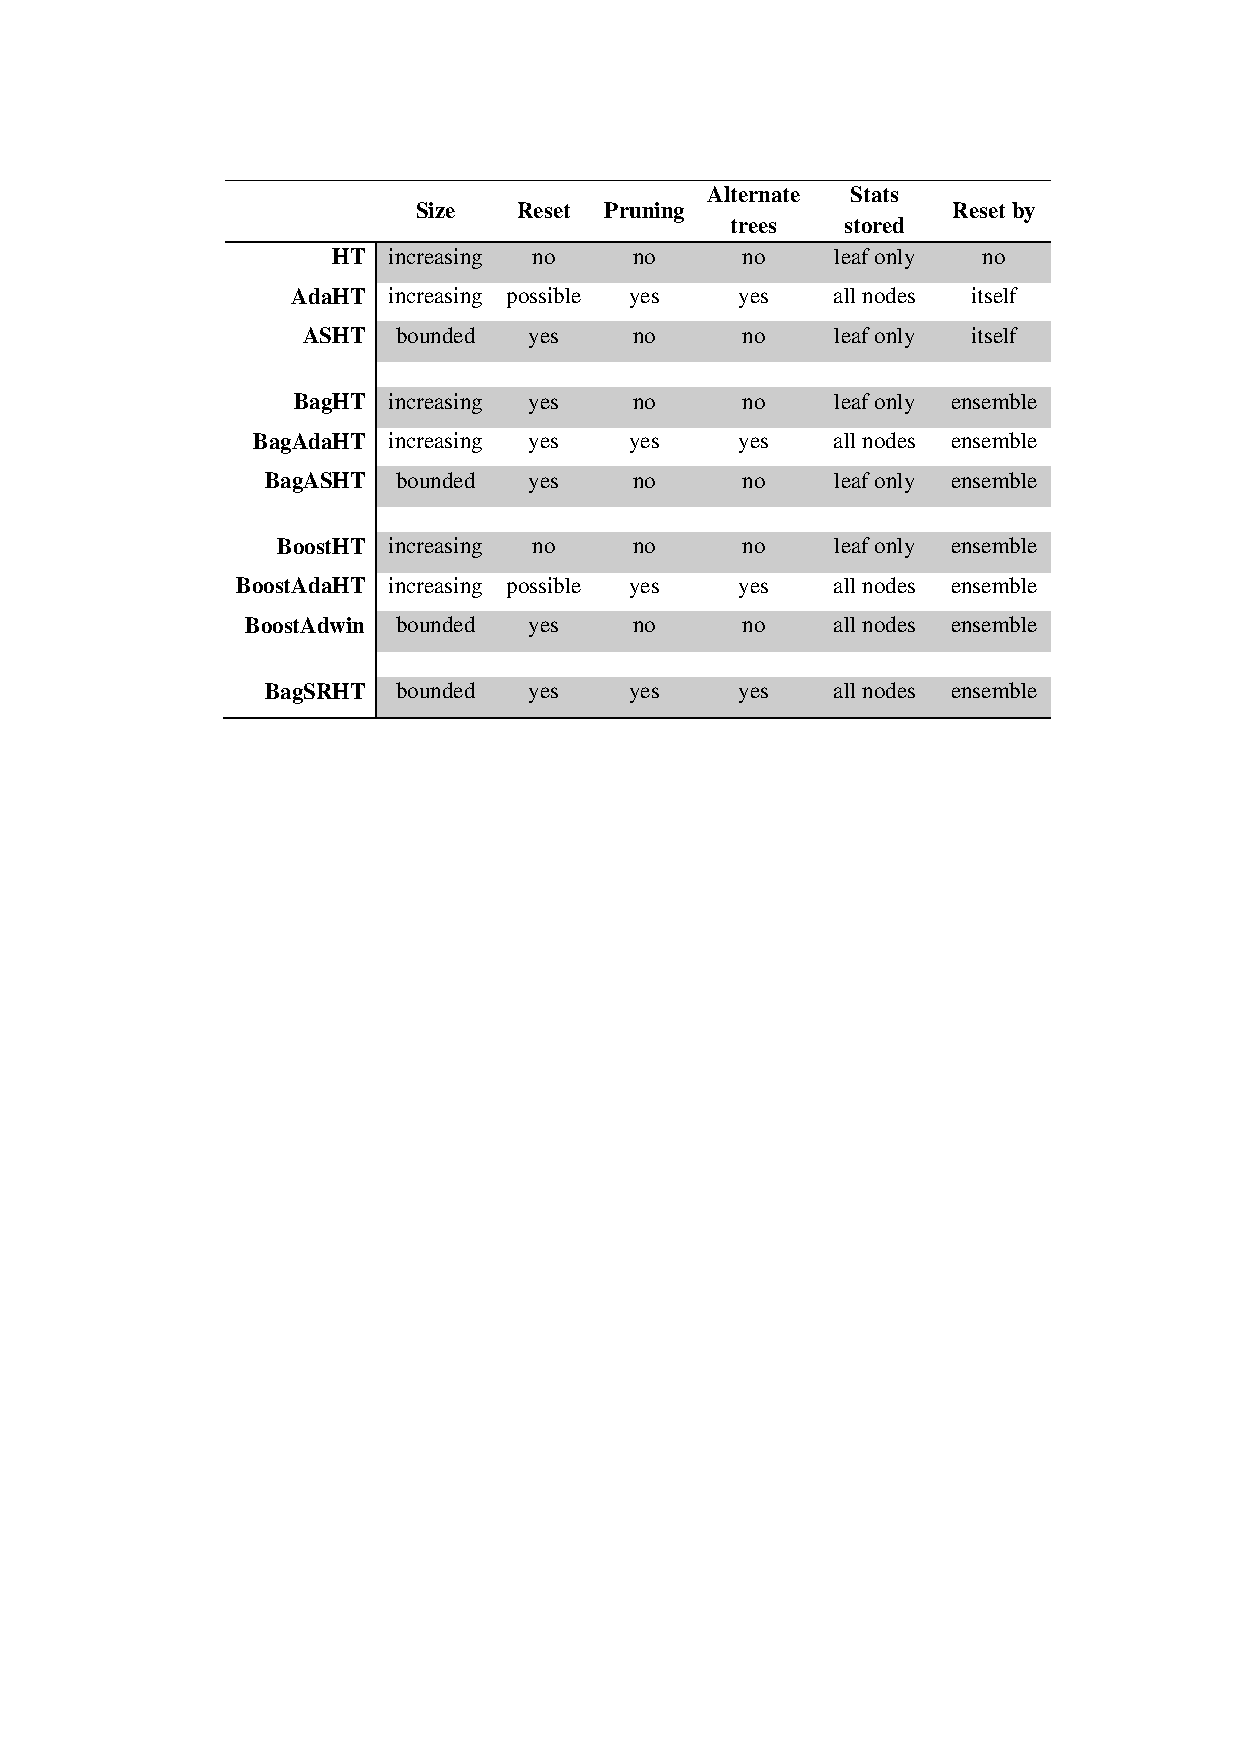
\includegraphics{figs/treescomp.pdf}
    \end{center}
\end{table}


\chapter{Experimental Evaluation}
\label{chp:exp}
In this chapter we present the empirical analysis of the discussed algorithms. We analyze the performances and properties of these algorithms varying a wide range of parameters. We compare our approach described in Chapter~\ref{chp:algo} with the current state-of-the-art methods presented in Chapter~\ref{chp:background}. Each of the analysis is performed simultaneously-- for both data streams generated by random RBF generator and our newer approach that generates speed varied RBF streams (Chapter~\ref{chp:dataset}). A 64-bit Windows 7 machine with Intel Core i7 dual-core processor clocking up to 2.4 GHz and 8 GB of RAM is used to run the experiments. The implementation is derived from Java based MOA framework~\cite{bifet:moa10}. 


\section{Evaluation Process}
There are two different approaches in evaluating algorithms in a streaming environment: (i) holdout evaluation, and (ii) prequential evaluation. In holdout evaluation, two separate train and test sets are used. Once the training is done, typically using one single-pass, on the training set, the test set is used to evaluate the performance. This is ideal where there are large amounts of data, where it is expected that with splitted test set, chances of over-fitting would be very low. In prequential evaluation, each example is first used to test the model in hand, and then the instance is used to train (update) the model. This method, thus, continuously changes the observed performance metrics and the model. A prequential model is, particularly, a necessity when the classifier has to ensure that the model is updated for the newest instances. The well-known cross validation approach is trivially not applicable in the streaming environment. In our settings, prequential evaluation is most appropriate. Binary class data sets of 1,000,000 instances in a 10 dimensional hyperspace are generated using the random RBF generator and the variable speed RBF generator for the evaluation. 

\subsection{Performance Metrics}
A number of metrics has been used for the evaluation criteria. Accuracy, processing time, memory usage, and kappa statistics are primarily used for the evaluation along with various tree structure related parameters such as tree depth, tree size, number of decision nodes, etc. Moreover, we observed algorithm specific properties e.g. number of tree reset, number of pruned trees, number of maintained alternate trees, number of times of partial tree replacement, etc. These algorithm specific parameters are not always directly comparable. Parameters are comparable among HT, adaptive HT, and ASHT. Bagging and boosting approaches have a different setting. Thus, we used weighted averages for these methods when calculating the number of resets or pruning type of statistics. For example, in bagging methods, smaller trees reset more often, thus while calculating the number of resets, a lower relative weight is given to the smaller trees. In our experiments, weights are proportional to the maximum size limits, or equal where there is no size restriction.

\subsection{Generalization Error Bound}
In batched leaning methods, the generalization error is a measurement that indicates how well a learning method generalizes to unseen data. It is the distance between the error on the training set and the test set, and is averaged over the entire set of possible training data for all iterations. In our stream mining environment, as we will be using prequential evaluation method, all samples would be first used as a test sample and then be used as a training sample. Moreover, as this will be performed only once, thus there would be no iteration over the training set, and the evaluation performance would be strongly tied with the sequence of  the incoming data. Thus, the notion of generalization error does not apply here. Rather, we focus on the confidence of the model being build. For Hoeffding tree based approaches, $\delta$ (Algorithm~\ref{alg:vfdt}, Algorithm~\ref{alg:srht}) is used to indicate an allowable error in each split decision. For our experiments, we kept this value to $0.0000001$. This is the maximum error to be accepted in a split decision. This is used to compute the Hoeffding bound, depending on which split decisions are taken.

\section{Study case: Census Income Dataset}
In the beginning, we check the performance of the stream algorithms in comparison to the classical batched data mining algorithms. For this evaluation, the census income data set~\cite{ron:adultds} is  used. This data set contains 48,842 instances of 14 attributes (6 continuous, 8 categorical) mapping to a binary ``income'' class (details in Appendix~\ref{appndx:ci}). With experimental evaluation, it is found that most batched learning methods such as C4.5, SVM, MLP achieve an accuracy around 82-83\% with 10 fold cross validation for the income class prediction task. As it can be seen from Figure~\ref{fig:exp:ci}, stream learning methods also achieve an accuracy within 1-2\% percent difference than the batched learners. Measured F1 values also presents similar scores. Though differences are insignificant, however, ASHT and bagging with ASHT seem to perform relatively worse than other algorithms. It is because of the resetting of the trees. After each reset, a few instances will suffer because the new trees are still very small. On the other hand, with our proposed modifications, bagging with SRHT overcomes this problem, and performs nearly the same as C4.5.

\begin{figure}[htbp] 
    \begin{center}
        \begin{tabular}{cc}
            \hspace{-3mm}\resizebox{75mm}{!}{\includegraphics{res/{0-ci-algo-accu}.pdf}} &
            
            \hspace{-5mm}\resizebox{75mm}{!}{\includegraphics{res/{0-ci-algo-fm}.pdf}} \\
            \scriptsize{(a)\vspace{2mm}} &
            \scriptsize{(b)}    
        \end{tabular}
        \caption{Comparison of batch and stream learning algorithms on census income data set with (a) accuracy and (b) F1-measure }
        \label{fig:exp:ci}
    \end{center}
\end{figure}


In terms of the tree structure, the final classifiers from a stream learner are simpler than the C4.5 tree. While C4.5 has many decision rules with over 10 decision nodes, Hoeffding tree based approaches are found to be performing similar with only 4 decision nodes. It is to note here that with a different ordering of the input data, a higher number of decision nodes is a possibility.

Lastly, we simulated a concept evolving scenario by controlled sampling of data from different clusters within the census income data. Five clusters were found using batched learning methods. While it had no significant effect on the performance of HT, however, methods that uses ADWIN are found to  get reset often depending on the sampling sequence. When each clusters is used sequentially, they reset all 4 times when concepts were changed.


\section{Impact of Parameters}
The evaluated algorithms depends on a number of parameters. Grace period, tie threshold, and tree type (binary or non-binary) are the most important parameters for HT, adaptive HT, and ASHT. For bagging and boosting methods the ensemble size is important. Additionally, for ASHT and SRHT, we have first classifier size, choice between reset and pruning are also important. Similarly, there are parameters on which the data generation processes (Chapter~\ref{chp:dataset}) rely on. In this section, we analyze the effect of each of these parameters starting with the parameters for data generation. For the discussion here, we used the most relevant metrics in respect to parameter. A comprehensive list of plots is given in the Appendix~\ref{appndx:plots} detailing all related metrics.

\subsection{Effect of Drift Coefficient}
Figure~\ref{fig:exp:speedxaccu}a suggests that the maximum deviation occurs within a value between 0.01 and 0.1. This is an implementation specific value, depending on the current MOA implementation. This is an indication that the drift coefficient changes the generation process periodically. That means after a threshold close to 0.05 drift reaches an amount that it starts forming clusters again. This agrees with previously seen cases. In Figure~\ref{fig:ds:rbfdrift} it was shown how generated data is distributed on a 2D space. Compared to Figure~\ref{fig:ds:rbfdrift}c, Figure~\ref{fig:ds:rbfdrift}d is denser.

\begin{figure}[htbp] 
    \begin{center}
        \begin{tabular}{cc}
            \hspace{-10mm} \resizebox{85mm}{!}{\includegraphics{res/{1-rnd-speed-accu}.pdf}} &
            \hspace{-10mm} \resizebox{85mm}{!}{\includegraphics{res/{1-vs-speed-accu}.pdf}} \\
            \scriptsize{(a)} & \scriptsize{(b)} \\
            
        \end{tabular}
        \caption{Effect of drift coefficient on accuracy using (a) random RBF (b) VSRBF}
        \label{fig:exp:speedxaccu}
    \end{center}
\end{figure}

For the random RBF stream, accuracy drops significantly for all algorithms with the introduction of drift in the system. In this range, bagging using ASHT and SRHT are the only two algorithms where no drift and very small drift have an insignificant (about 2\%) change. The accuracy of adaptive HT based approaches drop  the least, around 20\%; while HT suffers greatly with more than 30\% drop in accuracy. Performance improvement over bagging using ASHT with bagging using SRHT is insignificant (within 1-2\%).
\begin{figure}[htbp] 
    \begin{center}
        \begin{tabular}{cc}
            \hspace{-10mm} \resizebox{85mm}{!}{\includegraphics{res/{1-rnd-speed-time}.pdf}} &
            \hspace{-10mm} \resizebox{85mm}{!}{\includegraphics{res/{1-vs-speed-time}.pdf}} \\
            \scriptsize{(a)} & \scriptsize{(b)} \\
            
        \end{tabular}
        \caption{Effect of drift coefficient on processing time using (a) random RBF (b) VSRBF}
        \label{fig:exp:speedxtime}
    \end{center}
\end{figure}

For a variable speed RBF stream, this has less importance as the highest number of data is produced by a few centroids. The performance relies more on those specific centroids than on all centroids' drift. Thus, accuracy remains on the similar level with varying drift. Importantly though, there is  improvement in accuracy after drift introduction, contrary to its random RBF counterpart. One plausible explanation would be, with  the fewer drift centroids with higher data volume, it would cover more space, have higher decision rules, and thus achieve higher performance.

Next, on Figure~\ref{fig:exp:speedxtime} comparison of processing time for different drift coefficient is shown. As expected, classifiers that maintains higher number of trees, complete (SRHT bagging) or sub-trees (adaptive HTs), take longer time with drifting data. The reason is with drifting concepts, more alternate trees or bigger trees are needed to be maintained. For the same reason the tree depth, tree size, and memory show similar trends as the time plot (see Appendix~\ref{appndx:plots}).


\subsection{Effect of Number of Centroids}
The umber of generating centroids is another parameter for data generation. Each centroid in some way simulates concepts. We varied this number from 50 to 200 with steps of 50. No changes in terms of performance metrics is observed for random RBF data sets (Figure~\ref{fig:exp:centxaccu}a,~\ref{fig:exp:centxsize}a). For VSRBF streams a slight variation is observed, as depicted in Figure~\ref{fig:exp:centxaccu}b,~\ref{fig:exp:centxsize}b.

\begin{figure}[htbp] 
    \begin{center}
        \begin{tabular}{cc}
            \hspace{-10mm} \resizebox{85mm}{!}{\includegraphics{res/{3-rnd-centroid-accu}.pdf}} &
            \hspace{-10mm} \resizebox{85mm}{!}{\includegraphics{res/{3-vs-centroid-accu}.pdf}} \\
            \scriptsize{(a)} & \scriptsize{(b)} \\
            
        \end{tabular}
        \caption{Effect of number of centroids on accuracy using (a) random RBF (b) VSRBF}
        \label{fig:exp:centxaccu}
    \end{center}
\end{figure}

\begin{figure}[htbp] 
    \begin{center}
        \begin{tabular}{cc}
            \hspace{-10mm} \resizebox{85mm}{!}{\includegraphics{res/{3-rnd-centroid-tsize}.pdf}} &
            \hspace{-10mm} \resizebox{85mm}{!}{\includegraphics{res/{3-vs-centroid-tsize}.pdf}} \\
            \scriptsize{(a)} & \scriptsize{(b)} \\
            
        \end{tabular}
        \caption{Effect of number of centroids on tree size using (a) random RBF (b) VSRBF}
        \label{fig:exp:centxsize}
    \end{center}
\end{figure}

Tree sizes for all these algorithms fall into 3 general categories. Classifiers with size limitations (ASHT, SRHT) lies at the bottom of the plot, classifiers without any alternate tree maintenance scheme have higher tree sizes, however, those with alternate trees are about 5 times larger in sizes than these classifiers.

\begin{figure}[htbp] 
    \begin{center}
        \begin{tabular}{cc}
            \hspace{-10mm} \resizebox{85mm}{!}{\includegraphics{res/{4-rnd-driftcentroid-accu}.pdf}} &
            \hspace{-10mm} \resizebox{85mm}{!}{\includegraphics{res/{4-vs-driftcentroid-accu}.pdf}} \\
            \scriptsize{(a)} & \scriptsize{(b)} \\
            
        \end{tabular}
        \caption{Effect of percentage of drift centroid on accuracy using (a) random RBF (b) VSRBF}
        \label{fig:exp:driftxaccu}
    \end{center}
\end{figure}
\subsection{Effect of Percentage of Drifting Centroids}


In this set of experiments, we checked the effect of number of drifting centroids. Previously, we have shown the performance for different drifting amounts, and have found that with a relatively higher drifting rate (e.g. 0.01), performances of the algorithms drops substantially.  (Figure~\ref{fig:exp:speedxaccu}). For these experiments, we therefore, kept the drifting coefficient to 0.01 and varied percentage or drifting centroids from 20 to 100. As expected, accuracy and other metrics are found to be highly correlated with the percentage of drifting centroids till it reaches the random guess accuracy of 50\% (binary class problem). With 50\% of the centroids drifting with a coefficient of 0.01, performance reaches the minimum as shown in the Figure~\ref{fig:exp:driftxaccu}.


\subsection{Effect of Grace Period}
The grace period is the number of instances each node must receive before starting to check for split attribute. Thus, it is expected that with a higher grace period the algorithms will perform faster producing less decision nodes.


\begin{figure}[htbp] 
    \begin{center}
        \begin{tabular}{cc}
            \hspace{-10mm} \resizebox{85mm}{!}{\includegraphics{res/{2-rnd-grace-accu}.pdf}} &
            \hspace{-10mm} \resizebox{85mm}{!}{\includegraphics{res/{2-vs-grace-accu}.pdf}} \\
            \scriptsize{(a)} & \scriptsize{(b)} \\
            
        \end{tabular}
        \caption{Effect of grace period on accuracy using (a) random RBF (b) VSRBF}
        \label{fig:exp:gracexaccu}
    \end{center}
\end{figure}



\begin{figure}[htbp] 
    \begin{center}
        \begin{tabular}{cc}
            \hspace{-10mm} \resizebox{85mm}{!}{\includegraphics{res/{2-rnd-grace-time}.pdf}} &
            \hspace{-10mm} \resizebox{85mm}{!}{\includegraphics{res/{2-vs-grace-time}.pdf}} \\
            \scriptsize{(a)} & \scriptsize{(b)} \\
            
        \end{tabular}
        \caption{Effect of grace period on processing time using (a) random RBF (b) VSRBF}
        \label{fig:exp:gracextime}
    \end{center}
\end{figure}



\begin{figure}[htbp] 
    \begin{center}
        \begin{tabular}{cc}
            \hspace{-10mm} \resizebox{85mm}{!}{\includegraphics{res/{2-rnd-grace-tsize}.pdf}} &
            \hspace{-10mm} \resizebox{85mm}{!}{\includegraphics{res/{2-vs-grace-tsize}.pdf}} \\
            \scriptsize{(a)} & \scriptsize{(b)} \\
            
        \end{tabular}
        \caption{Effect of grace period on tree size using (a) random RBF (b) VSRBF}
        \label{fig:exp:gracexsize}
    \end{center}
\end{figure}

We varied the grace period from 200 (MOA default) to 3200 in a geometric rate of 2. Results for accuracy, processing time, and tree size are shown in Figure~\ref{fig:exp:gracexaccu}, \ref{fig:exp:gracextime}, and \ref{fig:exp:gracexsize} respectively. These figures show that for both random RBF and variable speed RBF, the effect of grace period is similar. Processing time and tree size drop  about 25\% to 33\% while the effect on accuracy is negligibly within 0-2\% only.


\subsection{Effect of Tie Threshold}
The tie threshold is used to break ties between two similarly good attributes for a split decision. If their gain difference in not greater than the Hoeffding margin, but the margin itself is less than tie threshold then a node is splitted on the best attribute at hand.

\begin{figure}[htbp] 
    \begin{center}
        \begin{tabular}{cc}
            \hspace{-10mm} \resizebox{85mm}{!}{\includegraphics{res/{5-rnd-tiethresh-accu}.pdf}} &
            \hspace{-10mm} \resizebox{85mm}{!}{\includegraphics{res/{5-vs-tiethresh-accu}.pdf}} \\
            \scriptsize{(a)} & \scriptsize{(b)} \\
            
        \end{tabular}
        \caption{Effect of tie threshold on accuracy using (a) random RBF (b) VSRBF}
        \label{fig:exp:tiexaccu}
    \end{center}
\end{figure}

A larger value for the tie threshold ensures that the margin between the best two attributes is higher. As Figure~\ref{fig:exp:tiexaccu} shows that the larger values yields better accuracy when we varied tie threshold from 0.001 to 0.1 with discrete intervals. However, in Figure~\ref{fig:exp:tiexsize}, it can be seen that this also increases the tree size substantially for adaptive HT based methods. Both random RBF and VSRBF show similar trends, but classifiers perform better on VSRBF. The reason is explained in the section above about effect of the drift coefficient. We used 0.01 as drift coefficients for these experiments.

\begin{figure}[htbp] 
    \begin{center}
        \begin{tabular}{cc}
            \hspace{-10mm} \resizebox{85mm}{!}{\includegraphics{res/{5-rnd-tiethresh-tsize}.pdf}} &
            \hspace{-10mm} \resizebox{85mm}{!}{\includegraphics{res/{5-vs-tiethresh-tsize}.pdf}} \\
            \scriptsize{(a)} & \scriptsize{(b)} \\
            
        \end{tabular}
        \caption{Effect of tie threshold on tree size using (a) random RBF (b) VSRBF}
        \label{fig:exp:tiexsize}
    \end{center}
\end{figure}

\subsection{Effect of Binary Split}
This set of experiments explores the effect of a binary split. This attribute has more importance in terms of tree structure than on the overall performance. The overall accuracy difference is negligible (about 1-2\%) for the non-binary and the binary tree. However, depth and number of decision nodes are greatly affected by this parameter. For example, tree sizes of adaptive HT based approaches drop  down from around 5000 nodes to under 1000 nodes when a binary splitting is used. Similarly, depths fall from around 25 to just 10. In Figure~\ref{fig:exp:binaryxaccu} we have shown the depths and tree sizes for a binary and non-binary split scenario for the random RBF generator. The variable speed RBF generator also produces similar results (see Appendix~\ref{appndx:plots}).

\begin{figure}[htbp] 
    \begin{center}
        \begin{tabular}{cc}
            \hspace{-10mm} \resizebox{85mm}{!}{\includegraphics{res/{6-rnd-binsplit-depth}.pdf}} &
            \hspace{-10mm} \resizebox{85mm}{!}{\includegraphics{res/{6-rnd-binsplit-tsize}.pdf}} \\
            \scriptsize{(a)} & \scriptsize{(b)} \\
            
        \end{tabular}
        \caption{Effect of binary split on (a) depth (b) tree size}
        \label{fig:exp:binaryxaccu}
    \end{center}
\end{figure}


\subsection{Effect of Ensemble Size}
The ensemble method has very little influence on static concepts. Figure~\ref{fig:exp:ensizexstatic} shows that for both random RBF and VSRBF generators increasing ensemble size achieves no better accuracy. But processing time increases linearly with increasing size.

\begin{figure}[htbp] 
    \begin{center}
        \begin{tabular}{cc}
            \hspace{-10mm} \resizebox{85mm}{!}{\includegraphics{res/{8-rnd-ensize-accu}.pdf}} &
            \hspace{-10mm} \resizebox{85mm}{!}{\includegraphics{res/{8-vs-ensize-time}.pdf}} \\
            \scriptsize{(a)} & \scriptsize{(b)} \\
            
        \end{tabular}
        \caption{Effect of ensemble size for static concepts on  (a) accuracy (b) processing time}
        \label{fig:exp:ensizexstatic}
    \end{center}
\end{figure}

However, with a small drift coefficient of 0.001, algorithms demonstrate  higher accuracy with the increasing ensemble size (Figure~\ref{fig:exp:ensizexdrift}). 


\begin{figure}[htbp] 
    \begin{center}
        \begin{tabular}{cc}
            \hspace{-10mm} \resizebox{85mm}{!}{\includegraphics{res/{8-rnd-ensize-accu-copy}.pdf}} &
            \hspace{-10mm} \resizebox{85mm}{!}{\includegraphics{res/{8-rnd-ensize-time}.pdf}} \\
            \scriptsize{(a)} & \scriptsize{(b)} \\
            
        \end{tabular}
        \caption{Effect of ensemble size for drifting concepts on  (a) accuracy (b) processing time}
        \label{fig:exp:ensizexdrift}
    \end{center}
\end{figure}

\subsection{Other Parameters}
Experiments are also performed for the maximum allowed size, the size of the first tree in an ensemble (other are multiples of the first one), and the reset vs pruning approaches. Their effect in our settings is found to be negligible. Evaluation plots are given in Appendix~\ref{appndx:plots}.


\section{Comparative Analysis of Timeline}
In the last section, we have presented performance metrics of the algorithms in terms of their parameters, and compared the algorithms based on the overall performance. However, with the final output of performances, we do not get the idea of how a tree reset or pruning affects the classifiers. Moreover, it is unclear that how bagging with SRHT is an improvement over bagging with ASHT. Thus, in this section, we present the analysis based on a windowed evaluation in a timeline manner. For this, we have used a windowed evaluation approach with 50,000 as the size of the window. Performances are sampled at each 50,000 instances. For this set of experiments, the used parameter values are: drift coefficient 0.001, grace period 200, tie threshold 0.05, percentage of drifting coefficient 100, ensemble size 5, binary split, and resettable. 

\subsection{Performance Over Time}

\begin{figure}[htbp] 
    \begin{center}
        \begin{tabular}{cc}
            \hspace{-10mm} \resizebox{85mm}{!}{\includegraphics{resw/{1-rnd-count-accu}.pdf}} &
            \hspace{-10mm} \resizebox{85mm}{!}{\includegraphics{resw/{1-vs-count-accu}.pdf}} \\
            \scriptsize{(a)} & \scriptsize{(b)} \\
            
        \end{tabular}
        \caption{Accuracy over time for (a) Random RBF (b) VSRBF}
        \label{fig:exp:taccu}
    \end{center}
\end{figure}


\begin{figure}[htbp] 
    \begin{center}
        \begin{tabular}{cc}
            \hspace{-10mm} \resizebox{85mm}{!}{\includegraphics{resw/{1-rnd-count-depth}.pdf}} &
            \hspace{-10mm} \resizebox{85mm}{!}{\includegraphics{resw/{1-vs-count-depth}.pdf}} \\
            \scriptsize{(a)} & \scriptsize{(b)} \\
            
        \end{tabular}
        \caption{Tree depth over time for (a) Random RBF (b) VSRBF}
        \label{fig:exp:tdeth}
    \end{center}
\end{figure}

Figure~\ref{fig:exp:taccu} shows the accuracy of the algorithms in different time of the window. Figure~\ref{fig:exp:tdeth} presents the depths of the trees at those corresponding times. For the random RBF generator, a lot of fluctuations in both accuracy (Figure~\ref{fig:exp:taccu}a) and tree depth (Figure~\ref{fig:exp:tdeth}a) can be seen. For the VSRBF generator, these fluctuations are bigger. The reason is presumably the high number of instances being generated from small number of concepts in VSRBF, and those concepts are constantly disappearing. However, an important thing to note here is the relationship between the drop in the depth and the drop in the accuracy for the random RBF generator, especially the bagging with a ASHT classifier. On the other hand, bagging with SRHT achieves a bit higher accuracy with a more stable classification rate. For VSRBF generator, bagging with ASHT seems to perform a little better than SRHT bagging but SRHT bagging is more stable. Some other classifiers are performing better (Figure~\ref{fig:exp:taccu}b), however, lead to an over-fitting scenario as the tree depth is constantly rising (Figure~\ref{fig:exp:tdeth}b).

This is essentially the goal of our new approach: to have a more stable ensemble such that deleting a classifier will not significantly affect accuracy for a certain period of time. Moreover,  Figure~\ref{fig:exp:pool} shows that bagging with SRHT improves performances for slower concepts (see Figure~\ref{fig:ds:varspd}).

\begin{figure}[htbp] 
    \begin{center}
            \resizebox{130mm}{!}{\includegraphics{resw/{0-vs-pool-accu}.pdf}}
            
        \caption{Accuracy within each data generating pool}
        \label{fig:exp:pool}
    \end{center}
\end{figure}

Among other metrics, the number of reset count found to be linearly increasing with time for both generators (Figure~\ref{fig:exp:treset}). Similarly, the processing time shows a linearly increasing trend over time (Figure~\ref{fig:exp:ttime}). Kappa statistics shows higher variations for VSRBF than for random RBF (Figure~\ref{fig:exp:tkappa}). 

\begin{figure}[htbp] 
    \begin{center}
        \begin{tabular}{cc}
            \hspace{-10mm} \resizebox{85mm}{!}{\includegraphics{resw/{1-rnd-count-reset}.pdf}} &
            \hspace{-10mm} \resizebox{85mm}{!}{\includegraphics{resw/{1-vs-count-reset}.pdf}} \\
            \scriptsize{(a)} & \scriptsize{(b)} \\
            
        \end{tabular}
        \caption{Number of tree being reset over time for (a) Random RBF (b) VSRBF}
        \label{fig:exp:treset}
    \end{center}
\end{figure}

\begin{figure}[htbp] 
    \begin{center}
        \begin{tabular}{cc}
            \hspace{-10mm} \resizebox{85mm}{!}{\includegraphics{resw/{1-rnd-count-time}.pdf}} &
            \hspace{-10mm} \resizebox{85mm}{!}{\includegraphics{resw/{1-vs-count-time}.pdf}} \\
            \scriptsize{(a)} & \scriptsize{(b)} \\
            
        \end{tabular}
        \caption{Processing time over time for (a) Random RBF (b) VSRBF}
        \label{fig:exp:ttime}
    \end{center}
\end{figure}


\begin{figure}[htbp] 
    \begin{center}
        \begin{tabular}{cc}
            \hspace{-10mm} \resizebox{85mm}{!}{\includegraphics{resw/{1-rnd-count-kappa}.pdf}} &
            \hspace{-10mm} \resizebox{85mm}{!}{\includegraphics{resw/{1-vs-count-kappa}.pdf}} \\
            \scriptsize{(a)} & \scriptsize{(b)} \\
            
        \end{tabular}
        \caption{Kappa over time for (a) Random RBF (b) VSRBF}
        \label{fig:exp:tkappa}
    \end{center}
    %\vspace{-5mm}
\end{figure}


\section{Discussion on the Experimental Evaluation}
We started this chapter by comparing stream learners with state-of-the-art batched learners. We showed that for the census income data set~\cite{ron:adultds} of about 49 thousand instances stream learners perform close to the best accuracies obtained by batched learners. This, however, cannot be used to conclude that stream learners would always show such a performance for other data sets.

Next, we have analyzed each of the algorithms including our new approach by varying the parameters within a wide range. We also have presented findings on the effect of different parameters of the data generation processes. It was found that the drift coefficient is inversely related with accuracy for 0 to 0.01, after which accuracy starts to increase again. Hence, this indicates that its effect on the data generation process is periodic. Performances of the learners are found to be nearly independent of the number of centroids used for a fairly high drift of 0.01. On the other hand, the percentage of drift centroids is inversely related to performance, and can bring accuracy down to the 50\% for a binary class problem with only 50\% drifting centroids. After that, increasing number of drifting centroids cannot not affect the classifier performance. 

From classifier parameters, a grace period is found to be very effective in reducing processing time and tree size, sacrificing a negligible amount of accuracy, which is essentially the motive to use a grace period. The use of higher threshold achieves higher accuracy while considerably increasing the tree size. It has also been shown that binary tree can achieve same accuracy but reducing tree size significantly. For ensemble based approaches, the ensemble size is found to be effective in drifting conditions while for the static conditions it had no effect. Other parameters have very little impact in our experimental setup.

Finally, we have presented the windowed performance evaluation or the timeline of performances of algorithms. It is here, where we can clearly distinguish and effectively prove the effectiveness of our new approach. While analyzing parameters, we have seen that bagging SRHT mostly performs better than bagging with ASHT. However, with the windowed analysis, we demonstrated how in ASHT bagging ensemble performs poorly after the trees being reset. Experimental results showed that SRHT bagging overcomes this issue and keeps a stable classifier though-out the time. Additionally, a breakdown of performance for different pools evidentially proved that SRHT is more effective for slower streams. Thus SRHT fairly realizes the motivation we presented at the beginning.




\chapter{Conclusion}
\section{Contribution}
\section{Future Works}
\section{Open Issues}

\bibliographystyle{apalike}
\addcontentsline{toc}{chapter}{Bibliography}
\bibliography{ref}


\chapter{Additional Plots}
\label{appndx:plots}
\section*{Parameter Analysis}
\begin{figure}[htbp] 
    \begin{center}
        \begin{tabular}{cc}
            
            \hspace{-5mm} \resizebox{80mm}{!}{\includegraphics{res/{1-rnd-speed-kappa}.pdf}} &
            \hspace{-10mm} \resizebox{80mm}{!}{\includegraphics{res/{1-vs-speed-kappa}.pdf}} \\
            \scriptsize{(c)} & \scriptsize{(f)} \\
            
        \end{tabular}
        \caption{Effect of drift coefficient on performance (a-c) random RBF (d-f) VS RBF}
        \label{fig:apndeffect:speed1}
    \end{center}
\end{figure}

\begin{figure}[htbp] 
    \begin{center}
        \begin{tabular}{cc}
            \hspace{-5mm} \resizebox{80mm}{!}{\includegraphics{res/{1-rnd-speed-depth}.pdf}} &
            \hspace{-10mm} \resizebox{80mm}{!}{\includegraphics{res/{1-vs-speed-depth}.pdf}} \\
            \scriptsize{(a)} & \scriptsize{(d)} \\
            
        \end{tabular}
        \caption{Effect of drift coefficient on structure (a-c) random RBF (d-f) VS RBF}
        \label{fig:apndeffect:speed2}
    \end{center}
\end{figure}
\begin{figure}[htbp] 
    \begin{center}
        \begin{tabular}{cc}
            
            \hspace{-5mm} \resizebox{80mm}{!}{\includegraphics{res/{1-rnd-speed-tsize}.pdf}} &
            \hspace{-10mm} \resizebox{80mm}{!}{\includegraphics{res/{1-vs-speed-tsize}.pdf}} \\
            \scriptsize{(b)} & \scriptsize{(e)} \\
            
        \end{tabular}
        \caption{Effect of drift coefficient on structure (a-c) random RBF (d-f) VS RBF}
        \label{fig:apndeffect:speed2}
    \end{center}
\end{figure}
\begin{figure}[htbp] 
    \begin{center}
        \begin{tabular}{ccc}
            \hspace{-5mm} \resizebox{80mm}{!}{\includegraphics{res/{1-rnd-speed-memory}.pdf}} &
            \hspace{-10mm} \resizebox{80mm}{!}{\includegraphics{res/{1-vs-speed-memory}.pdf}} \\
            \scriptsize{(c)} & \scriptsize{(f)} \\
            
        \end{tabular}
        \caption{Effect of drift coefficient on structure (a-c) random RBF (d-f) VS RBF}
        \label{fig:apndeffect:speed2}
    \end{center}
\end{figure}




\begin{figure}[htbp] 
    \begin{center}
        \begin{tabular}{cc}
            \hspace{-5mm} \resizebox{80mm}{!}{\includegraphics{res/{2-rnd-grace-depth}.pdf}} &
            \hspace{-10mm} \resizebox{80mm}{!}{\includegraphics{res/{2-vs-grace-depth}.pdf}} \\
            \scriptsize{(a)} & \scriptsize{(d)} \\
            
            
        \end{tabular}
        \caption{Effect of grace period on structure (a-c) random RBF (d-f) VS RBF}
        \label{fig:apndeffect:grace2}
    \end{center}
\end{figure}

\begin{figure}[htbp] 
    \begin{center}
        \begin{tabular}{cc}
            
            \hspace{-5mm} \resizebox{80mm}{!}{\includegraphics{res/{2-rnd-grace-memory}.pdf}} &
            \hspace{-10mm} \resizebox{80mm}{!}{\includegraphics{res/{2-vs-grace-memory}.pdf}} \\
            \scriptsize{(c)} & \scriptsize{(f)} \\
            
        \end{tabular}
        \caption{Effect of grace period on structure (a-c) random RBF (d-f) VS RBF}
        \label{fig:apndeffect:grace2}
    \end{center}
\end{figure}



\begin{figure}[htbp] 
    \begin{center}
        \begin{tabular}{cc}
            
            \hspace{-5mm} \resizebox{80mm}{!}{\includegraphics{res/{3-rnd-centroid-memory}.pdf}} &
            \hspace{-10mm} \resizebox{80mm}{!}{\includegraphics{res/{3-vs-centroid-memory}.pdf}} \\
            \scriptsize{(c)} & \scriptsize{(f)} \\
            
        \end{tabular}
        \caption{Effect of number of centroids on structure (a-c) random RBF (d-f) VS RBF}
        \label{fig:apndeffect:centroid2}
    \end{center}
\end{figure}



\begin{figure}[htbp] 
    \begin{center}
        \begin{tabular}{cc}
            
            \hspace{-5mm} \resizebox{80mm}{!}{\includegraphics{res/{4-rnd-driftcentroid-time}.pdf}} &
            \hspace{-10mm} \resizebox{80mm}{!}{\includegraphics{res/{4-vs-driftcentroid-time}.pdf}} \\
            \scriptsize{(b)} & \scriptsize{(e)} \\
            
        \end{tabular}
        \caption{Effect of percentage of drift centroids on performance (a-c) random RBF (d-f) VS RBF}
        \label{fig:apndeffect:driftcentroid1}
    \end{center}
\end{figure}
\begin{figure}[htbp] 
    \begin{center}
        \begin{tabular}{cc}
            \hspace{-5mm} \resizebox{80mm}{!}{\includegraphics{res/{4-rnd-driftcentroid-tsize}.pdf}} &
            \hspace{-10mm} \resizebox{80mm}{!}{\includegraphics{res/{4-vs-driftcentroid-tsize}.pdf}} \\
            \scriptsize{(b)} & \scriptsize{(e)} \\
            
            
        \end{tabular}
        \caption{Effect of percentage of drift centroids on structure (a-c) random RBF (d-f) VS RBF}
        \label{fig:apndeffect:driftcentroid2}
    \end{center}
\end{figure}
\begin{figure}[htbp] 
    \begin{center}
        \begin{tabular}{cc}
            
            \hspace{-5mm} \resizebox{80mm}{!}{\includegraphics{res/{4-rnd-driftcentroid-memory}.pdf}} &
            \hspace{-10mm} \resizebox{80mm}{!}{\includegraphics{res/{4-vs-driftcentroid-memory}.pdf}} \\
            \scriptsize{(c)} & \scriptsize{(f)} \\
            
        \end{tabular}
        \caption{Effect of percentage of drift centroids on structure (a-c) random RBF (d-f) VS RBF}
        \label{fig:apndeffect:driftcentroid2}
    \end{center}
\end{figure}



\begin{figure}[htbp] 
    \begin{center}
        \begin{tabular}{cc}
            
            \hspace{-5mm} \resizebox{80mm}{!}{\includegraphics{res/{5-rnd-tiethresh-time}.pdf}} &
            \hspace{-10mm} \resizebox{80mm}{!}{\includegraphics{res/{5-vs-tiethresh-time}.pdf}} \\
            \scriptsize{(b)} & \scriptsize{(e)} \\
            
            
        \end{tabular}
        \caption{Effect of tie threshold on performance (a-c) random RBF (d-f) VS RBF}
        \label{fig:apndeffect:tiethresh1}
    \end{center}
\end{figure}
\clearpage

\begin{figure}[htbp] 
    \begin{center}
        \begin{tabular}{cc}
            \hspace{-5mm} \resizebox{80mm}{!}{\includegraphics{res/{5-rnd-tiethresh-depth}.pdf}} &
            \hspace{-10mm} \resizebox{80mm}{!}{\includegraphics{res/{5-vs-tiethresh-depth}.pdf}} \\
            \scriptsize{(a)} & \scriptsize{(d)} \\
            
        \end{tabular}
        \caption{Effect of tie threshold on structure (a-c) random RBF (d-f) VS RBF}
        \label{fig:apndeffect:tiethresh2}
    \end{center}
\end{figure}

\begin{figure}[htbp] 
    \begin{center}
        \begin{tabular}{cc}
            \hspace{-5mm} \resizebox{80mm}{!}{\includegraphics{res/{6-rnd-binsplit-accu}.pdf}} &
            \hspace{-10mm} \resizebox{80mm}{!}{\includegraphics{res/{6-vs-binsplit-accu}.pdf}} \\
            \scriptsize{(a)} & \scriptsize{(d)} \\
            
        \end{tabular}
        \caption{Effect of binary split centroids on performance (a-c) random RBF (d-f) VS RBF}
        \label{fig:apndeffect:binsplit1}
    \end{center}
\end{figure}



\begin{figure}[H]
    \begin{center}
        \begin{tabular}{cc}
            \hspace{-5mm} \resizebox{80mm}{!}{\includegraphics{res/{6-rnd-binsplit-time}.pdf}} &
            \hspace{-10mm} \resizebox{80mm}{!}{\includegraphics{res/{6-vs-binsplit-time}.pdf}} \\
            \scriptsize{(b)} & \scriptsize{(e)} \\
            
        \end{tabular}
        \caption{Effect of binary split centroids on performance (a-c) random RBF (d-f) VS RBF}
        \label{fig:apndeffect:binsplit1}
    \end{center}
\end{figure}


\begin{figure}[htbp] 
    \begin{center}
        \begin{tabular}{cc}
            
            \hspace{-5mm} \resizebox{80mm}{!}{\includegraphics{res/{6-rnd-binsplit-memory}.pdf}} &
            \hspace{-10mm} \resizebox{80mm}{!}{\includegraphics{res/{6-vs-binsplit-memory}.pdf}} \\
            \scriptsize{(c)} & \scriptsize{(f)} \\
            
        \end{tabular}
        \caption{Effect of binary split on structure (a-c) random RBF (d-f) VS RBF}
        \label{fig:apndeffect:binsplit2}
    \end{center}
\end{figure}


\begin{figure}[htbp] 
    \begin{center}
        \begin{tabular}{cc}
            \hspace{-5mm} \resizebox{80mm}{!}{\includegraphics{res/{7-rnd-maxsize-accu}.pdf}} &
            \hspace{-10mm} \resizebox{80mm}{!}{\includegraphics{res/{7-vs-maxsize-accu}.pdf}} \\
            \scriptsize{(a)} & \scriptsize{(d)} \\
            
            
        \end{tabular}
        \caption{Effect of maximum allowed size of tree on performance (a-c) random RBF (d-f) VS RBF}
        \label{fig:apndeffect:maxsize1}
    \end{center}
\end{figure}
\begin{figure}[H] 
    \begin{center}
        \begin{tabular}{cc}
            \hspace{-5mm} \resizebox{80mm}{!}{\includegraphics{res/{8-rnd-ensize-depth}.pdf}} &
            \hspace{-10mm} \resizebox{80mm}{!}{\includegraphics{res/{8-vs-ensize-depth}.pdf}} \\
            \scriptsize{(a)} & \scriptsize{(d)} \\
            
            
        \end{tabular}
        \caption{Effect of ensemble size on structure (a-c) random RBF (d-f) VS RBF}
        \label{fig:apndeffect:ensize2}
    \end{center}
\end{figure}
\begin{figure}[htbp] 
    \begin{center}
        \begin{tabular}{cc}
            
            \hspace{-5mm} \resizebox{80mm}{!}{\includegraphics{res/{8-rnd-ensize-tsize}.pdf}} &
            \hspace{-10mm} \resizebox{80mm}{!}{\includegraphics{res/{8-vs-ensize-tsize}.pdf}} \\
            \scriptsize{(b)} & \scriptsize{(e)} \\
            
            
        \end{tabular}
        \caption{Effect of ensemble size on structure (a-c) random RBF (d-f) VS RBF}
        \label{fig:apndeffect:ensize2}
    \end{center}
\end{figure}

\begin{figure}[htbp] 
    \begin{center}
        \begin{tabular}{cc}
            \hspace{-5mm} \resizebox{80mm}{!}{\includegraphics{res/{9-rnd-ifreset-accu}.pdf}} &
            \hspace{-10mm} \resizebox{80mm}{!}{\includegraphics{res/{9-vs-ifreset-accu}.pdf}} \\
            \scriptsize{(a)} & \scriptsize{(d)} \\
            
        \end{tabular}
        \caption{Effect of tree reset (within ensemble) on performance (a-c) random RBF (d-f) VS RBF}
        \label{fig:apndeffect:ifreset1}
    \end{center}
\end{figure}


\begin{figure}[htbp] 
    \begin{center}
        \begin{tabular}{cc}
            \hspace{-5mm} \resizebox{80mm}{!}{\includegraphics{res/{10-rnd-firsttree-accu}.pdf}} &
            \hspace{-10mm} \resizebox{80mm}{!}{\includegraphics{res/{10-vs-firsttree-accu}.pdf}} \\
            \scriptsize{(a)} & \scriptsize{(d)} \\
            
            
        \end{tabular}
        \caption{Effect of first tree size centroids on performance (a-c) random RBF (d-f) VS RBF}
        \label{fig:apndeffect:firsttree1}
    \end{center}
\end{figure}

\clearpage
\section*{Comparative Analysis Over Timeline}

\begin{figure}[htbp] 
    \begin{center}
        \begin{tabular}{cc}
            \hspace{-5mm} \resizebox{80mm}{!}{\includegraphics{resw/{1-rnd-count-time}.pdf}} &
            \hspace{-10mm} \resizebox{80mm}{!}{\includegraphics{resw/{1-vs-count-time}.pdf}} \\
            \scriptsize{(a)} & \scriptsize{(d)} \\
            
            \hspace{-5mm} \resizebox{80mm}{!}{\includegraphics{resw/{1-rnd-count-tsize}.pdf}} &
            \hspace{-10mm} \resizebox{80mm}{!}{\includegraphics{resw/{1-vs-count-tsize}.pdf}} \\
            \scriptsize{(b)} & \scriptsize{(e)} \\
            
        \end{tabular}
        \caption{(a,d) time, (b,e) tree size, (c,f) kappa values over time for (a-c) random RBF, (d-f) VS RBF}
        \label{fig:apndeffect:wintime}
    \end{center}
\end{figure}

\clearpage


\chapter{Extended Related Works}
\label{appndx:erw}
\section*{Stream Learning}
In a recent approach, \cite{rutkowski13:vfdt} argued that using McDiarmid’s bound instead of Hoeffding bound in VFDT is more appropriate for ensuring the approximation bound i.e. the split decisions made after seeing certain number of instances will, with high probability, remain the same for infinite number of instances. The authors also presented McDiarmid’s bound for information gain of ID3 algorithm, and Gini index of CART algorithm. It is to be noted that Hoeffding bound is a special case of McDiarmid’s bound. In another paper, \cite{matuszyk:vfdt} showed usage of Hoeffding bound is mathematically flawed as (i) Hoeffding inequality only applies to arithmetic average, which information gain and Gini index are not, (ii) values obtained in sliding window methods are not independent, while Hoeffding inequality only applies to independent random variables. A revised bound showed that decision bound should be twice of the one given by Hoeffding bound, otherwise, error-likelihood should be updated accordingly.


A different decision tree based approach based on so-called \textit{Peano Count Tree (P-tree)} has been developed by Ding et al. for spatial data streams~\cite{ding02:peanocount}. The Peano Count Tree is a spatial data structure that facilitates a lossless compressed representation of spatial data. This structure is used for fast calculation of information gain for branching in decision trees.

Aggarwal et al. employs a slightly different idea in handling time-evolving data in their on demand classification approach of data streams ~\cite{aggarwal04:ondemand}. They used a modified \textit{micro-clusters concept} introduced in~\cite{aggarwal03:clustream}. Micro-clusters are created from the training data stream only. Each micro-cluster corresponds to a set of points from the training data belonging to the same class. To maintain statistics over different time horizons and avoid storage of unnecessary data points a geometric time frame is used. In the classification task, the \textit{$k$-nearest neighbor} based approach is taken, where micro-clusters are treated as node weighted by their instance counts. 

In~\cite{ganti02:gemm:focus} two algorithms named GEMM and FOCUS have been introduced for streams under block evolution. GEMM is used for model maintenance and FOCUS is for change detection between two data stream models. These algorithms have been tested using decision trees and frequent item set models. FOCUS uses bootstrapping methods to compute the distribution of deviation values when data characteristics remain the same. This distribution is then used to check whether the observed deviation value indicates a significant deviation. In another approach to handle concept drift, Last~\cite{last02:olin} proposed an online classification system OLIN that would dynamically adjust the size of the training window and the number of new examples between model re-constructions to the current rate of concept drift. OLIN uses constant resources to produce models, and achieves nearly the same accuracy as the ones that would be produced by periodically re-constructing the model from all accumulated instances.


In a different approach to handle concept drift Castillo et al.~\cite{gama03:drift} used Shewhart P-Charts in an online framework based on the idea of \textit{Statistical Quality Control}. Two alternatives of P-charts were used to monitor the stability of one or more quality characteristics in a drifting stream. The two alternatives only differed in the methods they estimate the target value to set the center. The group later introduced another drift detection scheme that monitors probability distribution of examples and maintains a online error rate to detect any concept drift~\cite{gama04:drift}. When distribution changes, error rate will increase. For stationary concept, the error rate should always gradually decrease. A new concept is said to be started if the error rate exceeds some predefined warning or threshold level. This approach has been used in \textit{Ultra Fast Forest Tree (UFFT)}~\cite{gama04:ft, gama05:ft} stream classification method. UFFT maintains naive Bayes statistics for every node. If at any node the error rate starts increasing, the node is pruned for drifting concept. UFFT uses similar approach and Hoeffding bound to control the growth of the tree. For each pair of classes a tree is maintained, hence it is called forest-of-trees.

Later, Aggarwal proposed another concept drift technique based on velocity density estimation \cite{aggarwal03:condrift}. Velocity density estimation is a technique to understand, visualize, and determine trends in the evolving data. The work presented a scheme to use velocity density estimation to create temporal velocity profiles and spatial velocity profiles at periodic instants in time. These profiles are then used to predict dissolution, coagulation, and shift in data. Proposed method could detect changes in trends in a single scan with linear order of number of data points. Additionally, a batch processing techniques to identify combinations of dimensions which results the greatest amount of global evolution are also introduced. In~\cite{kifer04:condrift} authors tried to formally define and quantify the change so that existing algorithms can precisely specify when and how the underlying distribution has changed. They employed a two fixed-length window model, where a current one is updated every time a new example arrives and a reference one is only updated when a change has been detected. To compare the distributions of the windows $L1$ distance has been used [confirm!read again]. Another method to compare two distribution has been presented in~\cite{dasu05:condrift} where authors used Kullback-Leibler (KL) distance to compare two distributions. KL distance is known to be related to the optimal error in determining the similarity of two distributions. In this non-parametric method no assumptions on the underlying distributions is required. 


\section*{Ensemble Learning}

Online bagging and boosting method do not particularly give attention to the concept drifting nature in the data. \textit{Accuracy Weighted Ensemble (AWE)}~\cite{wang03:accuweighted} is one of the earliest work on concept-drifting stream data. AWE assumes that the stream is delivered in chunks of defined size. With each incoming chunk, AWE updates its $k$ classifiers. Each classifier is associated a weight which is inversely proportional to the expected error of the respective classifier. To estimate this error, it is assumed that the distribution of test set is closest to the most recent chunks. Concept drift is adapted by effectively manipulating the number and the magnitude of the weights that are changing. An extension of AWE has been proposed in~\cite{brzezinski11:accuupdated}, namely \textit{Accuracy Updated Ensemble (AUE)}. AUE takes the weighting motivation from AWE, but improves the limitation of AWE. In AWE each classifier learns from the incoming chunks in a ``batched'' fashion. AUE employs an online scheme instead. AUE also adapts the weighting function to reduce the adverse effect in AWE of sudden drift in data. AWE weighting function is prone to suffer by rapid change in the stream and most or even all classifiers assuming they are ``risky''. This limitation has been addressed in AUE. Result shows that AUE performs marginally better than AWE, however, also requires slightly longer time and larger space.

%ens in stream

Another group of methods known as \textit{random forests} uses bagging of decision trees. The concept of random forest is introduced by Breiman~\cite{breiman99:randomforest}. Random forest works in a similar manner as bootstrap aggregation. However, for each split in the tree it only selects a subset of the features to be considered for splitting criterion. This \textit{feature bagging} approach helps avoiding very strong predictors to get selected over and over. One method mentioned before, \textit{Ultra Fast Forest Tree (UFFT)}~\cite{gama04:ft, gama05:ft} uses concepts of tree bagging, however, works with all features the whole time. UFFT maintains statistical information on each node to detect drift and grows the tree in a similar  approach to VFDT. Using the statistical information stored in nodes it detects concept drift with naive Bayes error-rate. Abdulsalam et al. proposed \textit{Dynamic Streaming Random Forests (DSRF)} focusing on lowering the number of examples required to build up new model in a drifting environment~\cite{salam08:dsrf, salam11:dsrf}. Shannon entropy~\cite{shannon01:entropy} is used to detect concept drift. All these methods are empirically proven to be effective for generalized scenario and chosen data sets. 


\clearpage

\chapter{Classical Learning Algorithms}
\label{appndx:cla}

\section*{Learning Algorithms}
The goal of data classification process is to predict an outcome based on some give data. In order to do so, data mining algorithms first processes a training set containing a set of attributes and corresponding outcome: a class or a value. Algorithms develop hypotheses that best describe the relationship among the attributes and the outcome for the total instance set.  Formally, learning problems are defined as follows: Given a data set of $m$ instances  $D \equiv \{ \{\vec{x}_1, y_1\}, \{\vec{x}_2, y_2\}, \{\vec{x}_3, y_3\}, \dots, \{\vec{x}_m, y_m\} \}$ where $ \vec{x} = \{x_1, x_2, x_3, \dots, x_n\}$, learning algorithms try to approximate $H \equiv y = f(\vec{x})$. Additional to being typical linear, polynomial, etc. functions, $H$ can also be a set of IF-THEN rules. These rules or functions are then used to predict unseen instances where outcome class is not known. These algorithms are known as learning algorithms, and in last few decades, have widely been researched in the field of machine learning. This section briefly discusses few of the basic algorithms upon which the foundation of ensemble methods and this thesis are laid. The detailed discussion of these algorithms are out of the scope of this chapter. Thus, we discuss only the core concepts here.

\subsection*{$k$-Nearest Neighbors}
$k$-nearest neighbor algorithm, in short $k$-NN, is one the simplest learning available. It is a non-parametric instance-based lazy learning algorithm and works for both supervised and unsupervised learning. It uses similarity measure like distance functions to classify unknown instances. The decision is a majority voting of  $k$ neighbors where $k$ is predefined. For example, if $k= 1$ then an unknown instance is assigned the class label of its nearest neighbor. There are several schemes to find the $k$ nearest neighbors. For continuous data, some well-known distance functions are Euclidean distance, Manhattan distance, Minkowski distance, etc.  As in Figure~\ref{fig:bg:knn} 1-NN classification for the new instance is {--}, 2-NN is undefined, 3-NN is {+} using Euclidean distance.
\begin{itemize}
    \item Euclidean distance $D_E = \sqrt{\sum_{\i =1 }^{k} (x_i - y_i)^2}$
    \item Manhattan distance $D_M = \sum_{\i =1 }^{k} |(x_i - y_i)|$
    \item Minkowski distance $D_{Mink}\sqrt[q]{\sum_{\i =1 }^{k} (|x_i - y_i|)^q}$
\end{itemize}
For categorical data, Hamming distance can be used. Hamming distance is defined as $D_H = \sum_{\i =1 }^{k} |(x_i - y_i)|$ where $|x_i - y_i|$ is $0$ if $x=y$, $1$ otherwise.

\begin{figure}[htbp]
    \begin{center}
        \includegraphics[width=3.0in]{figs/knn.pdf}
        \caption{Concept of $k$-NN}
        \label{fig:bg:knn}
    \end{center}
\end{figure}

Choosing an optimal $k$ is the prime challenge of $k$-NN algorithm, which is extremely training data dependent. Changing position of few training points could lead to a significant loss in performance. The method is particularly not stable in the class boundary. $k$ should be large enough that $k$-NN could overcome the noises in data, and small enough that instances of other classes are not included. Generally, higher $k$ reduces the overall noise and should be more precise. For most data set a value between $3$-$10$ performs much better than $1$-NN. Typically, cross-validation is used to determine a good $k$. 

\subsection*{Na\"ive Bayes}
Naive Bayes classification is based on Bayes rule. Bayes rule says that the probability of event $x$ conditioned on knowing event $y$, i.e. the probability of $x$ given $y$ is defined as
\[
p(x|y) = \frac{p(x,y)}{p(y)} = \frac{p(y|x) p(x)}{p(y)}
\]
The naive Bayes classifier~\cite{langley92:nb} assumes that all the explanatory variables are independent. Given a feature set $X = x_1, x_2, \dots, x_n$ of $n$ independent variables, naive Bayes assigns the instances to $k$ possible outcome or classes, $p(C_k | X)$. Using Bayes rule, the conditional probability can be decomposed as:
\[
p(C_k |X) = \frac{p(C_k) p(X|C_k)}{p(X)}.
\]
In other words,
\[
posterior = \frac{prior \times likelihood}{evidence}.
\]
Using chain rule repetitively, it can be expressed as follows:
\[
p(C_k |X) = p(C_k) \prod_{i=1}^n p(x_i | C_k)
\]
The predicted class is the one which maximizes the conditional probabilities $p(C_k|X)$, that is, classifier assigns the class label $\hat{y} = C_k$ for some $k$ that satisfies:
\[
\hat{y} = \underset{k \in \{1, \dots, K\}}{argmax}  p(C_k) \prod_{i=1}^n p(x_i | C_k)
\]

\subsection*{Decision Tree}
Decision trees (DTs) are another popular genre of non-parametric supervised learning algorithms. Trees allow a way to graphically organize a sequential decision process. Decision tree, a directed acyclic graph, contains decision nodes, each with branches for all alternate decisions. Leaf nodes are labeled with respective class label. Each path from root to leaf is a decision rule, consisting of conditional part (unions of all internal nodes' conditions) and a decision (of leaf node).

Decision trees use {\it information gain} to select the splitting attribute that would maximize the total entropy of each of the subtrees resulting from the spit. Entropy is a measurement of purity of an attribute, typically ranged between 0 and 1. A pure attribute, attribute with definitive value-class relationship, would have a low entropy and is easy to predict. On the other hand attribute with highly mixed value-class relationship would yield high entropy. A common entropy function is-
\[
entropy = - \sum_{i=1}^n p_i \lg p_i.
\]
where $p_1, p_2, \dots, p_n$ are the distributions of several class attributes and $\sum p_i = 1$. Information gain is the difference between old and new entropy after a split. This is good measurement of relevance of an attribute. However, in cases where an attribute can take on a large number of distinct values, information gain is not ideal. Presence of large set of values could uniquely identify the classes but also reduces chance to generalize unseen instance and should be avoided to be place near root.

Decision tree is, however, computationally feasible. Average cost of constructing a decision tree for $n$ instances with $m$ attributes is $O(mn \lg n)$, and querying time is $O(\lg n)$.

\subsection*{Neural Network}
The Neural Network (NN) is a learning method inspired by biological neural network. A set of inter-connected nodes (also known as perceptrons and neurons) mimics biological neural network. Figure~\ref{fig:bg:nnlayer} shows a skeleton of a neural network. Neural network is a weighted directed graph where a input layer is connected to the output layer via some layers of hidden layers. This is commonly known as Multi-Layer Perceptron (MLP). Decisions are made looking only into the output layer only. Hidden layers enlarge the space of hypotheses. If there is no hidden layer, then neural network becomes a simple regression problem i.e. output is a linear function of inputs. Each connection among these nodes has an associated weight. Given an input data set, these weights are updated accordingly to best fit the classification model. Learning is done by back-propagation algorithm~\cite{raul96:nn}. Errors are propagated back from the output layer to the hidden layer and weights are updated to minimize error.
\begin{figure}[htbp]
    \begin{center}
        \includegraphics[width=4.0cm]{figs/nnlayers.png}
        \caption{Neural network layers}
        \label{fig:bg:nnlayer}
    \end{center}
\end{figure}

Learning starts with assigning a small value as initial weights to all the connection weights. In case of a single perceptron, learning process is analogous to moving a parametric hyperplane around. Let $w_i$ be the weight of $i$-th input, then after $t+1$ iteration weight $w_i(t+1) = w_i(t) + \nabla E_i(t)$, where $\nabla E_i$ is the gradient of the error function. For a input vector $\mathbf{x}$ and true output $y$, $E$ is defined as the squared error:
\[
E = \frac{1}{2} Err^2 = \frac{1}{2} (y - h_w(\mathbf{x}))^2
\]
Thus gradient of $E$ would be:
\begin{align*}
    \nabla E = \frac{\partial E}{\partial W_j} & = Err \times \frac{\partial Err}{\partial W_j} = Err \times \frac{\partial}{\partial W_j} (y - g(\sum_{j=0}^n w_j x_j)) \\
    & = - Err \times g^{\prime} (in) \times x_j
\end{align*}
Based on this, weight update rule would be:
\[
w_j = w_j + \alpha \times Err \times g^{\prime} (in) \times x_j
\]
where $\alpha$ is learning rate coefficient. Back propagation algorithm for multi-layer perceptron also works in similar fashion. Weights in the output layer are updated using following equation:
\[
w_{j,i} = w_{j,i} + \alpha \times a_j \times \nabla_i
\]
where $\nabla_i = Err \times g^\prime(in_i)$. Hidden layers propagates this error from the output layer using:
\begin{align*}
    \nabla_j &= g^\prime (in_i) \sum_i w_{j,i} \nabla_i \\
    w_{k, j} &= w_{k, j} + \alpha \times a_k \times \nabla_j
\end{align*}

MLP is a very expressive method. Only $1$ hidden layer is sufficient to represent all continuous functions and $2$ can represent any functions. MLP is prone to local minima, which is avoided by running MLP multiple times with different initial weight settings.
\clearpage

\chapter{Census Income Dataset}
\label{appndx:ci}

Census income data set, also commonly known as adult data set has 48842 instances consisting of 14 attributes that map to a binomial Income class (<=50K or >50K). Attributes are age, sex, education, occupation, work class, working hours, marital status, relationship, country, race, final weight, capital gain, and capital loss. 2809 instance have missing values for either occupation or work class or both.

Occupation, education, marital status are the most important attributes. They can sufficiently classify the instance with an accuracy within 1\% of the accuracy achieved using all attributes. Education attribute has 16 values from pre-school to doctorate. 66\% of the instances belong to high-school grad, some college, and bachelor. Occupation attribute has 15 values. Instances are  more balanced for this attribute. Marital status consists of values from married, never married, and other status. The target income class is skewed towards <=50K class with 76\% of the instance.

Five primary clusters can be found in this dataset. Cluster 1 being mostly student groups, still studying and earning <= 50K. Cluster 2 are the young professionals, just started their career, and mostly earning less than 50K. Cluster 3 are the people with white collar jobs. People with bachelor or more education here earn >50K. Cluster 4 are the people with blue collar jobs, mostly earning <=50K. Cluster 5 are females. In this group too, people with bachelor or more degree earn >50K.

Most batched leaning algorithm achieves about 80-83\% accuracy with about 85-88\% F1 value.

\end{document}
